%\documentclass[12pt,a4paper,final]{article}
\documentclass[oneside]{diretrizes}            % Imprimir apenas frente
%\documentclass[doubleside]{diretrizes}        % Imprimir frente e verso

% Importações de pacotes
\usepackage[alf, abnt-emphasize=bf, recuo=0cm, abnt-etal-cite=2, abnt-etal-list=0]{abntex2cite}                      % Citações padrão ABNT
\usepackage[utf8]{inputenc}                         % Acentuação direta
\usepackage[T1]{fontenc}                            % Codificação da fonte em 8 bits
\usepackage{graphicx}                               % Inserir figuras
\usepackage{amsfonts, amssymb, amsmath}             % Fonte e símbolos matemáticos
\usepackage{booktabs}                               % Comandos para tabelas
\usepackage{verbatim}                               % Texto é interpretado como escrito no documento
\usepackage{multirow, array}                        % Múltiplas linhas e colunas em tabelas
\usepackage{indentfirst}                            % Endenta o primeiro parágrafo de cada seção.
\usepackage{microtype}                              % Para melhorias de justificação?
\usepackage[algoruled, portuguese]{algorithm2e}     % Escrever algoritmos
\usepackage{float}                                  % Utilizado para criação de floats
\usepackage{times}                                  % Usa a fonte Times

% Inclui o preâmbulo do documento
%
% Documento: Preâmbulo
%

\instituicao{Universidade Federal de Alagoas}
\abreviatura{UFAL}
\instituto{Instituto de Computação}
\departamento{Coordenadoria Institucional de Educação à Distância}
%\coordenadoria{Coordenadoria Institucional de Educação à Distância}
\local{Maceió/AL}
\programa{Curso de Graduação em Sistema de Informação}
\nomeautor{Carlos Roberto dos Santos Silva}
\titulotb{Aplicação de Técnicas de BI na SSP/AL (DISQUE DENÚNCIA)}
%\subtitulo{Subtítulo do trabalho}
\data{2020}
\grau{Bacharel}
\dataapresentacao{XX/XX/2020}

%Dados Orientador
\orientador{Fábio José Coutinho da Silva}
\instOrientador{Universidade Federal de Alagoas}
\departamentoorientador{Campus A.C.Simões}
\titulacaoorientador{Prof. Dr.}

%Dados Coorientador
%\coorientador{Debra Morgan}
%\instCoorientador{Universidade Federal de Alagoas}
%\departamentocoorientador{Campus Arapiraca}
%\titulacaocoorientador{Prof. Me.}

%Dados Examinador 1
\nmexamum{XXXXXX}
\instexamum{Universidade Federal de Alagoas}
\departamentoexamum{Campus A.C.Simões}
\titulacaoexamum{Prof. Me.}

%Dados Examinador 2
\nomeexamdois{YYYYYY}
\instexamdois{Universidade Federal de Alagoas}
\departamentoexamdois{Campus A.C.Simões}
\titulacaoexamdois{Prof. Me.}

% Define as cores dos links e informações do PDF
\makeatletter
\hypersetup{
    portuguese,
    colorlinks,
    linkcolor=black,
    citecolor=black,
    filecolor=black,
    urlcolor=black,
    breaklinks=true,
    pdftitle={\@title},
    pdfauthor={\@author},
    pdfsubject={\imprimirpreambulo},
    pdfkeywords={abnt, latex, abntex, abntex2}
}
\makeatother

% Redefinição de labels
\renewcommand{\algorithmautorefname}{Algoritmo}
\def\equationautorefname~#1\null{Equa\c c\~ao~(#1)\null}

% Cria o índice remissivo
\makeindex

% Início do documento
\begin{document}

    % Retira espaço extra obsoleto entre as frases.
    \frenchspacing

    % Elementos pré textuais
    \pretextual
    %
% Documento: Capa
%

\makeatletter
\begin{capa}
	\thispagestyle{empty}%limpa estilo da pagina
	\setlength{\baselineskip}{0.12\baselineskip}
    \begin{center} %Alinhamento centralizadoS
	
	
\includegraphics[scale=0.1]{./04-figuras/brasao-ufal.png}\\
	
	\vspace*{0.5cm}%Espaçamento entre linhas
    
    \textbf{\expandafter\uppercase\expandafter{\imprimirinstituicao}}\\
    \textbf{\expandafter\uppercase\expandafter{\imprimirinstituto}}\\
    \textbf{\expandafter\uppercase\expandafter{\imprimirdepartamento}}\\
    \textbf{\expandafter\uppercase\expandafter{\imprimirprograma}}\\
	
	\vspace*{5cm}%Espaçamento entre linhas
	\textbf{\expandafter\uppercase\expandafter{\imprimirnomeautor}}\\
	
	\vspace*{5cm}%Espaçamento entre linhas	
	\textbf{\expandafter\uppercase\expandafter{\imprimirtitulotb}}\\
	
	\vspace*{8cm}%%Espaçamento entre linhas
	\textbf{\expandafter\uppercase\expandafter{\imprimirlocal}}\\
	\textbf{\expandafter\uppercase\expandafter{\imprimirdata}}\\
		
	\end{center} %Alinhamento centralizado
\end{capa}
\makeatother

	

              % Capa
    %
% Documento: FOLHA DE ROSTO
%

\makeatletter
\begin{folhaderosto}
	\thispagestyle{empty}%limpa estilo da pagina
	
    \begin{center}
    
		\imprimirnomeautor\\
		\vspace*{8.2 cm}%Espaço entre linhas
		\imprimirtitulotb\\
		
    \end{center}
	
	\vspace*{0.35 cm}%Espaçamento entre linhas
		    \large%tamanho da fonte 
    		\hfill%Estica horizontamente  com espaços
	    	\begin{minipage}{8 cm}%Minipagina
	    		\begin{small} %Muda tamanho da fonte
	    		\setlength{\baselineskip}{0.7\baselineskip}
				
		    	{Monografia apresentada como requisito parcial para obtenção do grau de
		    	{\imprimirgrau } em {\imprimirprograma } da {\imprimirinstituicao}{ - }{\imprimirabreviatura},
		    	{\imprimirdepartamento}.}\\{
		    	}\\Orientador: {\imprimirtitulacaoorientador }{ }{\imprimirorientador}
				
				
				\end{small} %Muda tamanho da fonte
		    \end{minipage}%%Minipagina
		    	
		    \vspace*{10 cm}%Espaçamento entre linhas
		    
		    \begin{center} %Alinhamento centralizado
		    	\normalsize %Muda tamanho da fonte
	    		\imprimirlocal\\
	    		\imprimirdata
	    	\end{center}%Alinhamento centralizado

\end{folhaderosto}
\makeatother
        % Folha de rosto
    %
% Documento: FOLHA APROVAÇÃO
%

\makeatletter
\begin{folhadeaprovacao}

\thispagestyle{empty}%limpa estilo da pagina
	
	\begin{center}
    
		\imprimirnomeautor\\
		\vspace*{3.1 cm}%Espaço entre linhas
		\imprimirtitulotb\\
		
    \end{center}
	
	\vspace*{0.35 cm}%Espaçamento entre linhas
		    \large%tamanho da fonte 
    		\hfill%Estica horizontamente  com espaços
	    	\begin{minipage}{8 cm}%Minipagina
	    		\begin{small} %Muda tamanho da fonte
	    		\setlength{\baselineskip}{0.7\baselineskip}
				
		    	{Monografia apresentada como requisito parcial para obtenção do grau de
		    	{\imprimirgrau } em {\imprimirprograma } da {\imprimirinstituicao}{ - }{\imprimirabreviatura},
		    	{\imprimirdepartamento}.}\\{
		    	}\\				
				
				\end{small} %Muda tamanho da fonte
		    \end{minipage}%%Minipagina
		    	
		    \vspace*{0.6 cm}%Espaçamento entre linhas
		    
		    \large%%tamanho da fonte 
    		\hfill%%Estica horizontamente  com espaços
	    	 
		    
		    \normalsize %Muda tamanho da fonte
		    \vspace*{1.5 cm}%Espaçamento entre linhas
		    
		    \begin{minipage}{9 cm }%%Minipagina
		    {Data de Aprovação: {\imprimirdataapresentacao}}\\
		    \end{minipage}%Minipagina
			
			\begin{center}%Alinhamento centralizado
		    	\vspace*{1.21 cm}%Espaçamento entre linhas
				\textbf{Banca Examinadora}\\ %Negrito
						
				\vspace*{1.2 cm}%Espaçamento entre linhas
				\rule{9 cm}{.1 mm}\\
				{\imprimirtitulacaoorientador}{ }{\imprimirorientador}\\
				{\imprimirinstOrientador}\\
				{\imprimirdepartamentoorientador}\\
				Orientador\\

				\vspace*{1.1 cm}%Espaçamento entre linhas
				\rule{9 cm}{.1 mm}\\
				\imprimirtitulacaoexamum{ }\imprimirnmexamum\\
				\imprimirinstexamum\\
				\imprimirdepartamentoexamum\\
				Examinador\\
				
				\vspace*{1.1 cm}%Espaçamento entre linhas
				\rule{9 cm}{.1 mm}\\				
								
				\imprimirtitulacaoexamdois{ }\imprimirnomeexamdois\\
				\imprimirinstexamdois\\
				\imprimirdepartamentoexamdois\\
				Examinador
				\vspace*{1.3 cm}%Espaçamento entre linhas
		    \end{center}%Alinhamento centralizado


\end{folhadeaprovacao}
\makeatother
    % Folha de aprovação
    %
% Documento: Dedicatória
%

\thispagestyle{empty}
\begin{dedicatoria}

Aqui você pode inserir uma homenagem ou dedica seu trabalho.

\end{dedicatoria}
       % Dedicatória
    % Documento: Agradecimento


\begin{agradecimento}

A todos os meus familiares por sempre me apoiarem, mesmo não entendendo muitas vezes o meu afastamento para estudar e pesquisar. Em especial à Minha mãe que nos deixou para ficar ao lado de Deus este ano; aos meus Filhos Caynan Eduardo e Carla Eduarda, pois, são a razão das minha lutas diárias e principalmente a Deus "Todo Poderoso" e seu Filho Jesus Cristo, por me dar: força, determinação, paciência, resiliência e paz todos os dias de minha vida.
Aos meus amigos e fãs da Plataforma de Integração de Dados e Análise Pentaho: Prof. Me. Thiago Araújo Silva de Oliveira, Mestre em Ciências da Computação pela UFPE, especialista em Pentaho, e aos Tenente PM Sidcley e ao Cabo PM Jamerson Dias Ramos, gestores de estatística do NEAC (Núcleo de Estatística e Análise Criminal) por proporcionarem ajudas técnicas especializadas em BI, para que eu concluísse esse trabalho.
Ao Sr Tenente Coronel QOC PM Marcelo da Rocha Nogueira, Assessor da AII/SSP-AL (Assessoria de Inteligência da Secretaria de Segurança Pública)  por liberar o acesso aos dados do 181, para que estes fossem trabalhados na monografia.
Ao Sr, Major QOC PM Roberto Feliciano co-fundador do 181 em nosso Estado, maior mente por trás do 18.1 atual ex-gestor do Núcleo de Disque Denúncia/All (Assessoria de Inteligência da Secretaria de Segurança Pública)  dar acesso aos dados do 181, para que os dados fossem trabalhados na monografia.
Ao meu orientador o Prof. Dr. Fábio José Coutinho da Silva, pelos incentivos, conselhos, ensinamentos e paciência durante todo período de desenvolvimento de trabalho de conclusão de curso.
A AII/SSP (Assessoria Integrada de Inteligência),  por ter disponibilizado acesso a base de dados do SISGOU.
Aos nossos professores do curso EAD-BSI-UFAL da Universidade Aberta do Brasil do polo de Maceió/AL, que contribuíram para os conhecimento adquiridos por este discente durante os períodos deste excelente curso.


\end{agradecimento}

    % Agradecimentos
    %
% Documento: Epígrafe
%
\thispagestyle{empty}
\begin{epigrafe}


O fator decisivo para vencer o maior obstáculo é, invariavelmente, ultrapassar o obstáculo anterior.{\\}{\\}

\begin{autorepigrafe}
Henry Ford
\end{autorepigrafe}

\end{epigrafe}


          % Epígrafe
    %
% Documento: Resumo (Português)
%

\begin{RESUMO}
\thispagestyle{empty}
	\begin{SingleSpace}
	
		\hspace{-1.2 cm}Este trabalho de conclusão visa a implementação de um BI tradicional, baseado nos dados gerados pelas denúncias registradas no canal 181, disque denúncia (via: telefone, web e aplicativo), com foco na coleta, extração e organização de dados para permitir o processamento eficiente de consultas para obter percepções de dados históricos que irão auxiliar aos tomadores de decisões na elaboração de um policiamento ostensivo e preventivo, com mais eficácia e eficiência, dentro da Estrutura da Segurança Pública de Alagoas. O BI propõe um \textit{Fontend} para as informações de forma simples através da utilização da Plataforma de Integração de Dados e Análise Pentaho. O objetivo desta monografia foi alcançado, tendo as informações disponibilizadas aos gestores de uma forma gráfica, facilitando a análise dos dados. Neste trabalho usamos estratégias como a linguagem de Expressões Multidimensionais (MDX) que é uma linguagem de consulta para processamento analítico online (OLAP) usando um sistema de gerenciamento de banco de dados (SGDB), que exploram e manipulam os dados que geram informações relevantes para a organização em questão. Esses sistemas permitem a organização, análise, compartilhamento e monitoramento de informações que oferecem suporte à gestão de negócios, fazendo com que cada gestor tome decisões importantes com mais rapidez. Essa técnica de negócio descreve as habilidades das corporações para acessar os dados e explorar as informações, normalmente contidas em uma data warehouse.


		\vspace*{0.5cm}\hspace{-1.3 cm}\textbf{Palavras-chave}: \textit{Business Intelligence} (BI). \textit{Data Warehouse} (DW). MultiDimensional eXpressions (MDX). \textit{Online Analytical Processing} (OLAP).
		
		
		
	\end{SingleSpace}
\end{RESUMO}


          % Resumo na língua vernácula
    %
% Documento: Resumo (Inglês)
%

\begin{ABSTRACT}
	\begin{SingleSpace}
	
		\hspace{-1.3 cm}This conclusion work aims to implement a traditional BI, based on the data generated by the complaints registered in channel 181, dial the complaint (via: phone, web and application), with a focus on the collection, extraction and organization of data to allow efficient processing consultations to obtain perceptions of historical data that will assist decision makers in developing ostentatious and preventive policing, more effectively and efficiently, within the Public Security Framework of Alagoas. BI proposes a Font-end for information in a simple way through the use of the Data Integration and Analysis Pentaho Platform. The objective of this monograph was achieved, having the information made available to managers in a graphic way, facilitating data analysis. In this work we use strategies such as the Multidimensional Expressions language (MDX), which is a query language for online analytical processing (OLAP) using a database management system (SGDB), which explore and manipulate the data that generate relevant information for the organization in question. These systems allow the organization, analysis, sharing and monitoring of information that support business management, making each manager make important decisions faster. This business technique describes the ability of corporations to access data and explore information, which is normally contained in a data warehouse.


		\vspace*{0.5cm}\hspace{-1.3 cm}\textbf{Keywords}: Business Intelligence (BI). Data Warehouse (DW). MultiDimensional eXpressions (MDX). Online Analytical Processing (OLAP).
		
		
	\end{SingleSpace}

\end{ABSTRACT}
          % Resumo em língua estrangeira
    %
% Documento: Lista de figuras
%

\pdfbookmark[0]{\listfigurename}{lof}
\listoffigures*
\cleardoublepage

      % Lista de figuras
    %
% Documento: Lista de tabelas
%

\pdfbookmark[0]{\listtablename}{lot}
\listoftables*
\cleardoublepage
      % Lista de tabelas
    %
% Documento: Lista de quadros
%

\pdfbookmark[0]{\listofquadrosname}{loq}
\listofquadros*
\cleardoublepage
      % Lista de quadros
    %
% Documento: Lista de abreviaturas e siglas
%

\begin{siglas}
	\setlength{\baselineskip}{0.7\baselineskip}
	
    \item[181] Número telefônico do serviço disque denúncia da SSP/AL
    \item[ABNT] Associação Brasileira de Normas Técnicas
    \item[AII] Assessoria Integrada de Inteligência
    \item[BI] \textit{Business Intelligence}
    \item[CSO] Diretor de Estratégia
    \item[DM] \textit{Data Mining}
    \item[DW] \textit{Data Warehouse}
    \item[EIS] \textit{Executive Information Systems}
    \item[ETL] \textit{Extract Transform Load}
    \item[MDX] \textit{Multidimensional Expressions}
    \item[MIT] \textit{Massachusetts Institute of Technology}
    \item[NBR] Norma Brasileira
    \item[OLAP] \textit{On-Line Analytics Processing}
    \item[OLTP] \textit{Online Transaction Processing}
    \item[PCP] Processo e Controle de Produção
    \item[RAM] \textit{Random Access Memory}
    \item[SAD] Sistema de Apoio à Decisão
    \item[SGBD] Sistema de Gerenciamento de Banco de Dados
    \item[SI] Sistema Integrado
    \item[SIE] Sistemas de Informação Executiva
    \item[SIG] Sistemas de Informações Gerenciais
    \item[SPT] Sistemas de Processamento de Transações
    \item[SQL] \textit{Structured Query Language}
    \item[SSP] Secretaria de Segurança Pública
    \item[SSP/AL] Secretaria de Segurança Pública do Estado de Alagoas
    \item[TCC] Trabalho de Conclusão do Curso
    \item[XML] \textit{Extensible Markup Language}
    
\end{siglas}
       % Lista de abreviaturas e siglas
    %
% Documento: Lista de símbolos
%

\begin{simbolos}
    \item[$ \Gamma $] Letra grega Gama
    \item[$ \lambda $] Comprimento de ondada
    \item[$ \in $] Pertence
\end{simbolos}
     % Lista de símbolos
    \sumario

    % Elementos textuais
    \textual
    %
% Documento: Introdu\c{c}\~{a}o
%

\chapter{INTRODU\c{c}\~{a}O}\label{chap:introducao}

O cenário atual dos negócios objetiva a diferenciação e a busca por um desempenho com base na eficiência, seja em uma organiza\c{c}\~{a}o pública ou privada, dar-se-\'{a} por meio da utilização de ferramentas e recursos, que visam a otimiza\c{c}\~{a}o das atividades, paralelamente à redução de seus custos.

Assim, na \'{a}rea da seguran\c{c}a pública e por intermédio dos elementos da tecnologia de informação, é possível registrar, armazenar e ter acesso de maneira eficaz, organizada e estruturada as informações sobre uma grande massa de dados de denúncias e ocorrências em cidades, bairros com datas e horas. Desta forma, tendências podem ser analisadas com base nesses dados, viabilizando a aplica\c{c}\~{a}o de determinado tipo de policiamento e ajudando na gestão da própria seguran\c{c}a pública, além de permitir uma melhor interlocução dos participantes da SSP.

\section{Apresenta\c{c}\~{a}o}

Na \'{a}rea da seguran\c{c}a pública e por intermédio dos elementos da tecnologia de informação, é possível registrar, armazenar e ter acesso de maneira eficaz, organizada e estruturada as informações sobre uma grande massa de dados de denúncias e ocorrências em cidades, bairros com datas e horas. Desta forma, tendências podem ser analisadas com base nesses dados, viabilizando a aplica\c{c}\~{a}o de determinado tipo de policiamento e ajudando na gestão da própria seguran\c{c}a pública, além de permitir uma melhor interlocução dos participantes da SSP.

Neste trabalho aplicamos as t\'{e}cnicas de Kimbal (2013)\cite{dw-kimball-2013} apresentadas em sua obra \textit{The Data Warehouse Toolkit}, no desenvolvimento de um BI que atue no banco de dados que registra as informa\c{c}ões das denúncias para ampliar a habilidade de planejar e auxiliar \`{a} tomada de decisões estrat\'{e}gicas no âmbito da Secretaria de Seguran\c{c}a Pública do Estado de Alagoas. 

Neste trabalho, propõe-se aplicar essa t\'{e}cnica com o uso de ferramentas modernas tal como o Pentaho \index{NewR}\footnote{Pentaho: Plataforma ou Software da Empresa Hitachi, composta por v\'{a}rias ferramentas que empregam as t\'{e}cnicas de BI.} na base de dados de denúncias registradas. Utilizaremos uma amostra de dados que abrangem os três primeiros meses do ano de 2020, os mesmo foram pesquisados e salvos no formato do \textit{Microsoft Excel}, que passaram pelo processo de extra\c{c}\~{a}o, transforma\c{c}\~{a}o e leitura e ao final termos um conjunto complexo de informa\c{c}ões que ajudar\~{a}o na tomada de decis\~{a}o.

% Disque Denúncia
\section{História do Disque Denúncia}		

Desde sua implanta\c{c}\~{a}o em Alagoas, em outubro de 2011, o Disque-Denúncia tem se revelado uma ferramenta útil para a popula\c{c}\~{a}o, que passou a contar com um meio seguro e sigiloso para relatar denúncias diversas.
Atrav\'{e}s do número telefônico 181, \'{e} possível denunciar ocorrências de criminalidade com a garantia do sigilo de quem passa a informa\c{c}\~{a}o. Al\'{e}m disso, o servi\c{c}o atua em denúncias referentes \`{a} venda ilegal de g\'{a}s de cozinha, tr\'{a}fico de drogas, posse e porte ilegal de arma de fogo, localiza\c{c}\~{a}o de foragidos e pessoas envolvidas com roubo a banco e pr\'{a}tica de homicídio.

Ele \'{e} gerido pela Secretaria de Seguran\c{c}a Pública, o número 181 \'{e} uma central de atendimento a recep\c{c}\~{a}o de chamadas telefônicas com denúncias de crimes e delitos que tem como objetivo agilizar o atendimento \`{a} popula\c{c}\~{a}o e contribuir para a redu\c{c}\~{a}o da criminalidade no Estado. \'{e} um servi\c{c}o gratuito e totalmente sigiloso. Por isso, o anonimato, al\'{e}m de um direito, se torna um dever da central desse servi\c{c}o, para garantir a seguran\c{c}a do cidad\~{a}o denunciante.

O anonimato \'{e} garantido porque, as liga\c{c}ões para o Disque Denúncia n\~{a}o s\~{a}o identificadas, rastreadas ou gravadas. Ao ligar para o 181, o usu\'{a}rio receber\'{a} uma senha num\'{e}rica chamada código da denúncia. Esta ser\'{a} a referência dele em caso do mesmo precisar acompanhar o andamento da investiga\c{c}\~{a}o, ou trazer novas informa\c{c}ões sobre o caso.

No SisGOU, os dados aparecem no módulo Disque Denúncia, eles s\~{a}o vindos do site do disque denúncia ser\'{a} apresentado nas próximas se\c{c}ões. Esses dados das denúncias,  guardando o sigilo e identifica\c{c}\~{a}o de quem entra em contato com o servi\c{c}o, que pode ser atrav\'{e}s do ``APP 181'', disponível na \textint{Play Store} \index{NewR}\footnote{Play Store: \'{e} uma loja virtual que j\'{a} vem pr\'{e}-instalada em aparelhos certificados, permitindo o acesso ao conteúdo digital, incluindo aplicativos, jogos, filmes, músicas e livros.} e no portal do servi\c{c}o, conforme figura abaixo, assim pode-se realizar denúncias via celular ou \textit{tablet}, pela internet ou liga\c{c}\~{a}o para o número 181, esse último sendo o mais conhecido, auxiliando no controle das denúncias e no envio das mesmas para as Unidades e Companhias de Polícia Militar e para as Delegacias, por\'{e}m n\~{a}o possui nenhuma ferramenta de inteligência de negócios integrada ao sistema, que venha orientar os gestores na tomada de decisões. 

### Figuras
\begin{figure}[H]
	\vspace*{0,2cm}
    \centering
    \caption{Disque Denúncia \textit{Mobile}}
    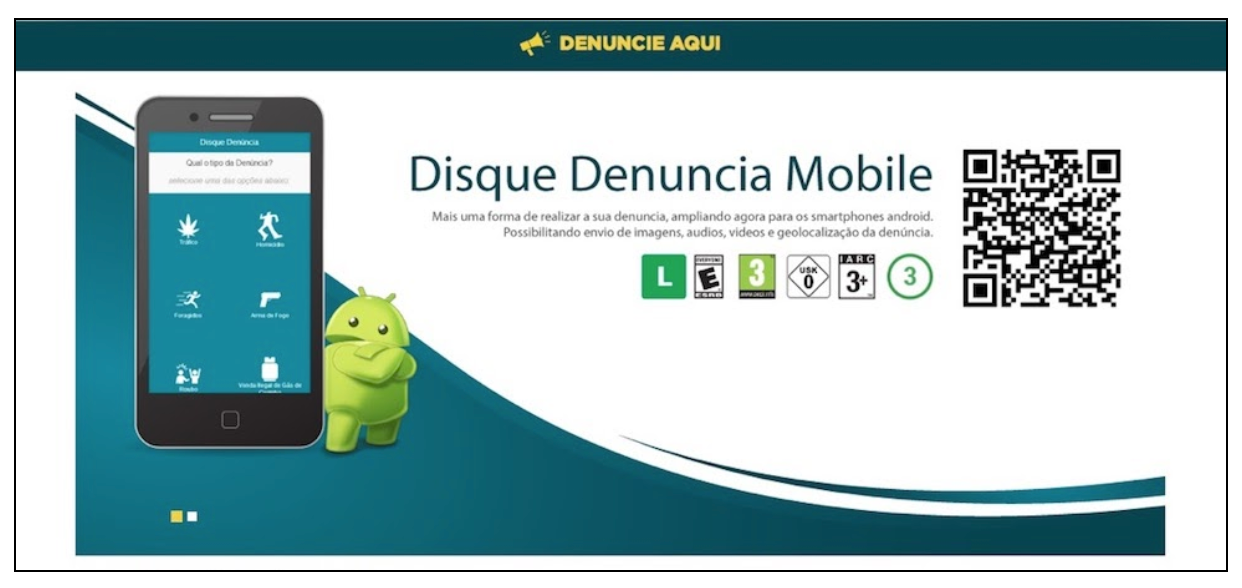
\includegraphics[width=0.6\textwidth]{./04-figuras/figura-disque-denuncia}
    \label{fig:ilustfigdisquedenuncia}
\end{figure}
\vspace*{-0,9cm}
{\raggedright \fonte{Autor desta monografia, 2020.}} \\

A partir dos dados do Disque-Denúncia, com base nos últimos seis anos, 63\% das liga\c{c}ões se referem a fatos em Maceió. Desde a implanta\c{c}\~{a}o desse servi\c{c}o, que funciona 24 horas, registra-se aumento anual no número de denúncias. At\'{e} 2011, havia uma m\'{e}dia de sete ao dia. Em 2016 este dado subiu para 42 (quarenta e dois) registros di\'{a}rios, sendo um acr\'{e}scimo de 5\% em rela\c{c}\~{a}o a 2017 nas informa\c{c}ões passadas pela popula\c{c}\~{a}o, hoje se tornando uma ferramenta importante para a SSP/AL.

% Objetivo Geral
\subsection{Objetivo geral}

O objetivo deste trabalho é desenvolver e implantar um modelo de \textint{Data Warehouse} Corporativo com base nos dados provindos do Aplicativo SISGOU da SSP/AL que cont\'{e}m os dados do 181, aplicando t\'{e}cnicas de DW/BI, Segundo KIMBALL (2013)\cite{dw-kimball-2013}.

% Objetivo Específico
\subsection{Objetivos específicos}

Os objetivos específicos do presente trabalho de pesquisa s\~{a}o:

\begin{itemize}

    \item Revisar as literaturas que abrangem os principais conceitos de BI; 
    \item Identificar problemas e benefícios com relação à implementação da tecnologia  \textint{e data warehouse};
    \item Definir um repositório de dados históricos para auxiliar os gerentes, contendo informações relevantes para a tomada de decisões com base nos dados armazenados;
    \item Extrair informações da base de dados do SISGOU, integrá-las e armazená-las em um repositório único central de \textint{Data Warehouse};
    \item Definir os níveis de granularidades necessários para a distribuição dos dados dentro deste modelo dimensional distribuído;
    \item Repassar à sociedade os conhecimentos e resultados obtidos nesta pesquisa.

\end{itemize}

% Resultados esperados
\section{Resultados Esperados}

Os resultados esperados s\~{a}o:

\begin{itemize}

    \item Após aplicarmos as t\'{e}cnicas de KIMBALL (2013) termos um DW funcional;
    \item Explorar o DW criado com as t\'{e}cnicas acima para prover informa\c{c}ões gerenciais;
    \item Aplicar estas informa\c{c}ões gerenciais para melhorar o Policiamento Ostensivo;
    \item Prover pain\'{e}is \textint{(Dashboards)} eficientes e que ajudem com informa\c{c}ões que auxiliem nas tomadas de decisões
    \item Tornar esse trabalho como base para o uso de recursos de BI para ajudar na seguran\c{c}a pública.

\end{itemize}
    %
% Documento: Fundamenta\c{c}\~{a}o
%

\chapter{FUNDAMENTA\c{c}\~{a}O}\label{chap:fundamentacao}

Neste cap\'{i}tulo apresentaremos as pesquisas bibliogr\'{a}ficas, para a fundamenta\c{c}\~{a}o te\'{o}rica que nos permite termos a base para alcan\c{c}ar os objetivos estabelecidos para este trabalho.

Al\'{e}m dos principais conceitos sobres os temas abordados neste trabalho como: Sistemas de informa\c{c}\~{a}o, BI, conhecimentos sobre fontes de dados, ETL, DW, DM, KDD, OLAP, Cubo, Data mining e um hist\'{o}rico sobre o servi\c{c}o 181 (disque denúncia) s\~{a}o necess\'{a}rios para a aplica\c{c}\~{a}o, desenvolvimento de um BI funcional e bem dimensionado.

\section{Sistemas de informa\c{c}\~{a}o}

Um sistema de informa\c{c}\~{a}o \'{e}um conjunto interdependente de pessoas, estruturas organizacionais, software, hardware, processos e m\'{e}todos interligados com o objetivo de facilitar o planejamento e o controle em empresas e outras organiza\c{c}\~{o}es, organizando informa\c{c}\~{o}es de forma que estas se tornem utiliz\'{a}veis na coordena\c{c}\~{a}o do fluxo de trabalho de uma empresa \cite{si-laudon-laudon}.

\subsection{SPT (Sistemas de processamento de transa\c{c}\~{o}es)}

Os sistemas de processamento de transa\c{c}\~{o}es, representam a aplica\c{c}\~{a}o dos conceitos e tecnologia de informa\c{c}\~{a}o em transa\c{c}\~{o}es rotineiras, repetitivas e geralmente comuns de neg\'{o}cios \cite{si-stair-1998}. Uma transa\c{c}\~{a}o pode ser entendida como um evento que ocorre num neg\'{o}cio tal como compra, venda, pagamento, entre outros.

Os sistemas de processamento de transa\c{c}\~{o}es possuem foco no n\'{i}vel operacional da empresa, armazenando e processando fluxos de dados pertinentes a automa\c{c}\~{a}o de processos de modo que estes sejam mais planejados e otimizados, visando garantir a integra\c{c}\~{a}o e normaliza\c{c}\~{a}o, possuindo, em sua grande maioria, alguns relat\'{o}rios para gerenciamento.

\subsection{SIG (Sistemas de informa\c{c}\~{o}es gerenciais)}

Sistema de Informa\c{c}\~{a}o Gerencial \'{e}o processo de transforma\c{c}\~{a}o de dados em informa\c{c}\~{o}es que ser\~{a}o utilizadas na estrutura decis\'{o}ria da empresa, bem como proporcionar\~{a}o a sustenta\c{c}\~{a}o administrativa para otimizar os resultados esperados \cite{si-oliveira-1998}.

\begin{flushleft}
	Estes sistemas têm o prop\'{o}sito de fornecer informa\c{c}\~{o}es necess\'{a}rias \`{a} medi\c{c}\~{a}o da eficiência operacional da organiza\c{c}\~{a}o, dando ênfase \`{a}s necessidades gerenciais atrav\'{e}s de informa\c{c}\~{o}es resumidas, obtidas a partir da filtragem e an\'{a}lise de dados altamente detalhados, extra\'{i}dos das bases de dados dos sistemas de processamento transacionais e de fontes \cite{si-stair-1998} \cite{si-falsarella-chaves-1998}.
\end{flushleft}

\subsection{SAD (Sistemas de apoio \`{a} decis\~{a}o)}

Os Sistemas de Apoio \`{a} Decis\~{a}o, s\~{a}o sistemas que realizam o processamento anal\'{i}tico e provêem as informa\c{c}\~{o}es necess\'{a}rias ao usu\'{a}rio, permitindo a an\'{a}lise de situa\c{c}\~{o}es e a tomada de decis\~{o}es \cite{si-inmon-1997}.

Os processamentos anal\'{i}ticos dos SAD permitem ao usu\'{a}rio analisar uma grande quantidade de dados, normalmente hist\'{o}ricos, verificando problemas e situa\c{c}\~{o}es, de modo a identificar perfis, tendências e padr\~{o}es, sendo a performance das consultas ou extra\c{c}\~{o}es de dados importantes, por\'{e}m n\~{a}o crucial no desenvolvimento deste tipo de aplica\c{c}\~{a}o.

\subsection{SIE (Sistemas de informa\c{c}\~{a}o executiva)}

Os Sistemas de Informa\c{c}\~{a}o executiva, s\~{a}o um tipo especial de SAD destinado \`{a} tomada de decis\~{o}es de alto n\'{i}vel da organiza\c{c}\~{a}o, oferecendo informa\c{c}\~{o}es estruturadas, tanto internas quanto externas a respeito de aspectos da organiza\c{c}\~{a}o considerados fatores \cite{si-stair-1998} \cite{si-falsarella-chaves-1998}.

Enquanto um SAD oferece apoio para decis\~{o}es focadas em uma \'{a}rea espec\'{i}fica, geralmente oferecendo suporte \`{a} m\'{e}dia e baixa ger\^{̂e}ncia, um EIS (Executive Information Systems) oferece informa\c{c}\~{o}es consolidadas de alto n\'{i}vel e an\'{a}lises multidimensionais para os executivos de alto n\'{i}vel \cite{si-gupta-2001}.

\section{BI (Business Intelligence)}

A Origem do Termo \textit{Business Intelligence} (BI) foi utilizado pela primeira vez na d\'{e}cada de 50 por \textit{Hans Peter Luhn}, um pesquisador da IBM, no artigo intitulado “A Business Intelligence System” \cite{bi-elena-2011}. O autor prop\~{o}e o desenvolvimento de sistema autom\'{a}tico, baseado em m\'{a}quinas de processamento de dados, que indexa e codifica automaticamente documentos e dissemina informa\c{c}\~{o}es nas organiza\c{c}\~{o}es conforme o ponto de a\c{c}\~{a}o.

Assim em 1989, \textit{Howard Dresner}, um membro de pesquisa do \textit{Gartner Group} popularizou “BI” com um termo gen\'{e}rico, usado para descrever um conjunto de conceitos e m\'{e}todos para aperfei\c{c}oar a tomada de decis\~{o}es de neg\'{o}cios utilizando sistemas de suporte baseados em fatos.

Dresner deixou o \textit{Gartner} em 2005 e entrou para a \textit{Hyperion Soluctions} como seu CSO (\textit{Chief Strategic Officer} – Diretor de Estrat\'{e}gia).

J\'{a} \cite{bi-cortes-2008} afirma que o \textit{Business Intelligence} (BI ou intelig\^{e}ncia empresarial) est\'{a} relacionado \`{a} habilidade de compreender, entender e ter o conhecimento necess\'{a}rio do pr\'{o}prio neg\'{o}cio de modo que as suposi\c{c}\~{o}es possam ser realizadas com grande chance de sucesso e que possam ter resultados satisfat\'{o}rios.

Para \cite{dw-kimball-2013} o sistema DW/BI deve tornar as informa\c{c}\~{o}es facilmente acess\'{i}veis. O conteúdo do sistema DW/BI deve ser compreens\'{i}vel. Os dados devem ser intuitivos e \'{o}bvios para o usu\'{a}rio comercial, n\~{a}o apenas para o desenvolvedor. As estruturas e os r\'{o}tulos dos dados devem imitar os processos e o vocabul\'{a}rio dos usu\'{a}rios de neg\'{o}cios. Os usu\'{a}rios corporativos desejam separar e combinar dados anal\'{i}ticos em infinitas combina\c{c}\~{o}es.

Em s\'{i}ntese, na figura abaixo, h\'{a} uma descri\c{c}\~{a}o como o BI pode ser entendido, como uma metodologia que permite transformar dados em informa\c{c}\~{o}es qualificadas, gerando conhecimento para a tomada de decis\~{o}es.

\begin{figure}[H]
	\vspace*{0,2cm}
    \centering
    \caption{Ilustra\c{c}\~{a}o da estrutura}
    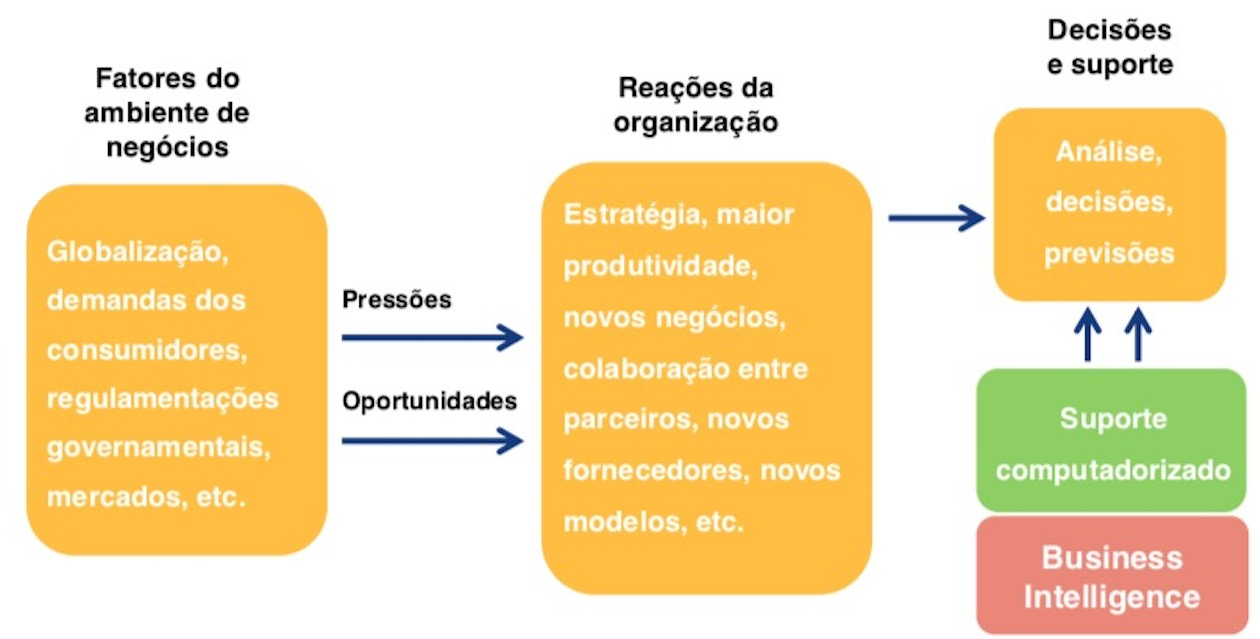
\includegraphics[width=0.6\textwidth]{./04-figuras/figura-01}
    \label{fig:ilustfig01}
\end{figure}
\vspace*{-0,9cm}
{\raggedright \fonte{Dispon\'{i}vel em: <https://Portal (www.fp2.com.br)>. Acesso em: 10 ago. 2020.}}\\

\subsection{A arquitetura e componentes}

Como j\'{a} mencionado temos como base os estudos de \cite{dw-kimball-2013}, seus elementos de arquitetura est\~{a}o representados na figura abaixo, como ilustrado, para \cite{dw-kimball-2013}, existem quatro componentes separados e distintos a serem considerados no ambiente DW/BI: sistemas de origem operacional, sistema ETL, \'{a}rea de apresenta\c{c}\~{a}o de dados e aplicativos de intelig\^{e}ncia de neg\'{o}cios.

\begin{figure}[H]
	\vspace*{0,2cm}
    \centering
    \caption{Elementos principais da arquitetura Kimball DW/BI.}
    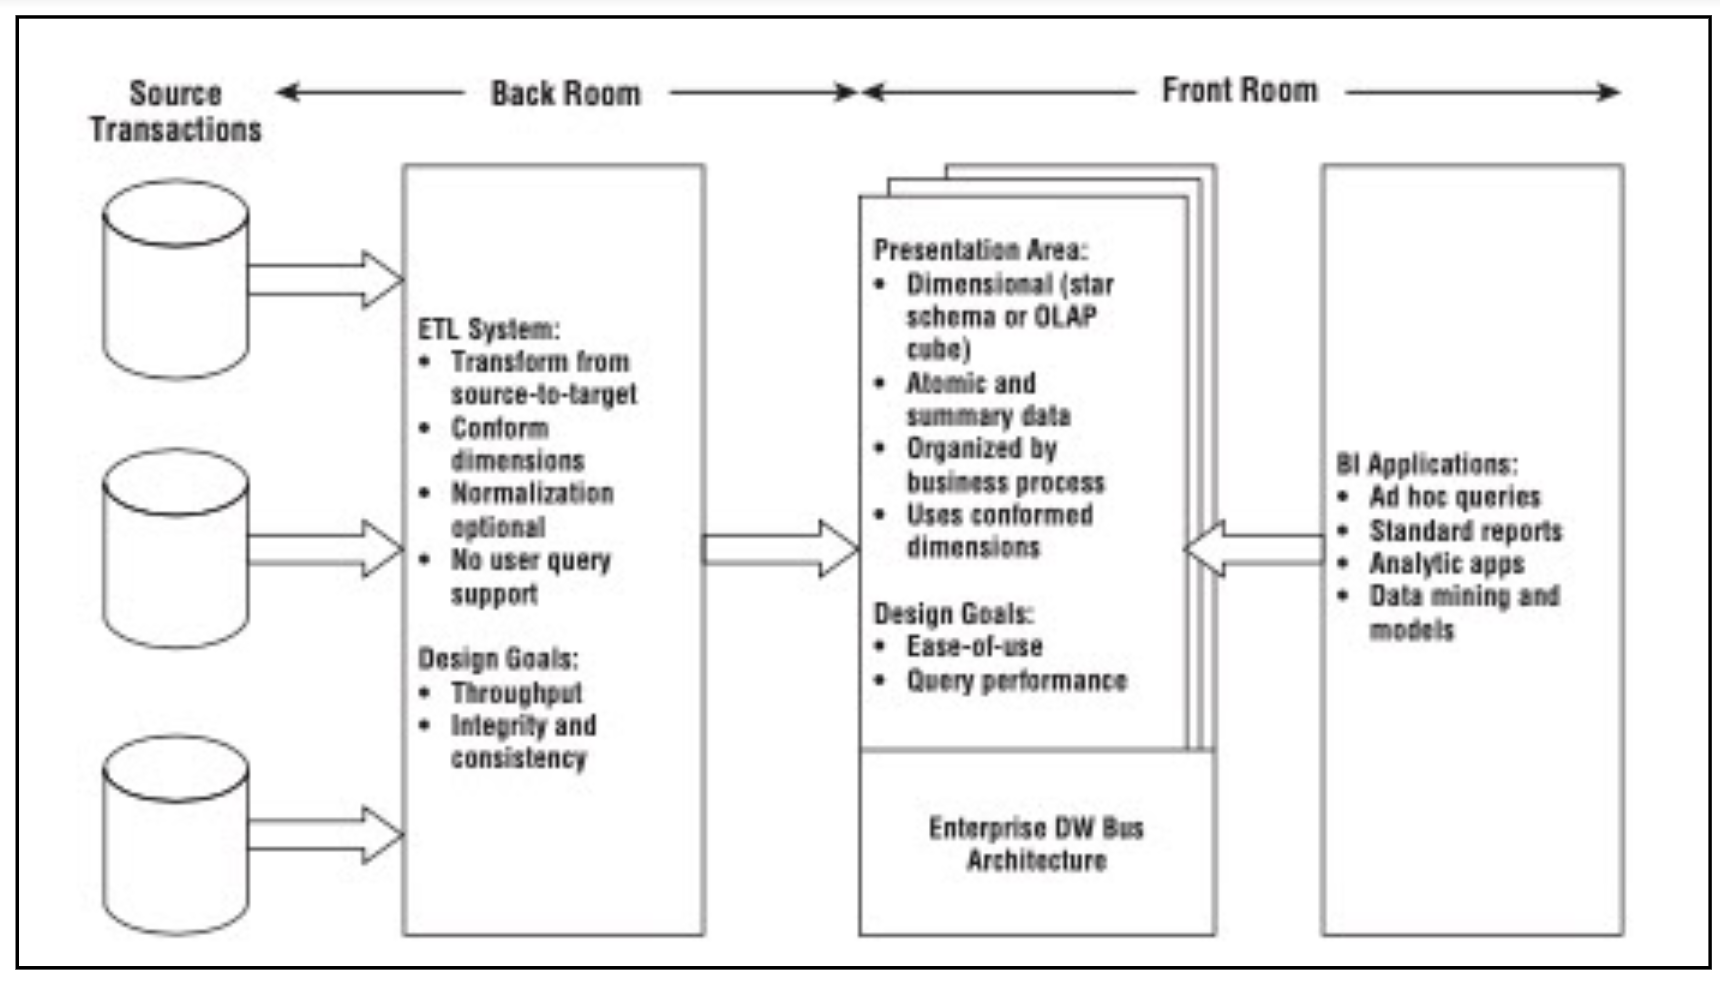
\includegraphics[width=0.6\textwidth]{./04-figuras/figura-02}
    \label{fig:ilustfig02}
\end{figure}
\vspace*{-0,9cm}
{\raggedright \fonte{ \textit{Core elements of the Kimball DW/BI architecture,} \cite{dw-kimball-1998}}}\\

O primeiro dele \'{e} o \textit{Operational Source Systems} que s\~{a}o os sistemas operacionais de registro ou origem que capturam as transa\c{c}\~{o}es da empresa. Pense nos sistemas de origem como fora do \textit{Data Warehouse}, porque, presumivelmente voc\^{e} tem pouco ou nenhum controle sobre o conteúdo e o formato dos dados nesses sistemas operacionais. 

As principais prioridades dos sistemas de origem s\~{a}o o desempenho e a disponibilidade do processamento. As consultas operacionais em rela\c{c}\~{a}o aos sistemas de origem s\~{a}o consultas estreitas, um registro por vez, que fazem parte do fluxo normal da transa\c{c}\~{a}o e severamente restringidas em suas demandas no sistema operacional.

O segundo \'{e} o ETL (\textit{Extract, Transformation, and Load System}) s\~{a}o os sistemas respons\'{a}veis pela: extra\c{c}\~{a}o, transforma\c{c}\~{a}o e carregamento. E que consiste em uma \'{a}rea de trabalho, estruturas de dados instanciadas e um conjunto de processos.

A cria\c{c}\~{a}o de estruturas normalizadas para o ETL e estruturas dimensionais para apresenta\c{c}\~{a}o, significa que os dados s\~{a}o potencialmente extra\'{i}dos, transformados e carregados duas vezes - uma vez no banco de dados normalizado e depois novamente quando voc\^{e} carrega o modelo dimensional. 
A terceira \'{e} \textit{Presentation Area to Support Business Intelligence} \'{e} nela onde os dados s\~{a}o organizados, armazenados e disponibilizados para consulta direta por usu\'{a}rios, redatores de relat\'{o}rios e outros aplicativos de BI anal\'{i}ticos.

A quarta \'{e} o \textit{Business Intelligence Applications} que \'{e} o componente final da arquitetura Kimball DW/BI. \'{e} o aplicativo de \textit{Business Intelligence} (BI) composto de uma variedade de recursos fornecidos aos usu\'{a}rios de neg\'{o}cios para alavancar a \'{a}rea de apresenta\c{c}\~{a}o para tomada de decis\~{a}o anal\'{i}tica.

Um aplicativo de BI pode ser t\~{a}o simples quanto uma ferramenta de consulta \textit{ad hoc} ou t\~{a}o complexo quanto um aplicativo sofisticado de minera\c{c}\~{a}o ou modelagem de dados. 

As ferramentas de consulta \textit{ad-hoc}, por mais poderosas que sejam, podem ser entendidas e usadas efetivamente apenas por uma pequena porcentagem da popula\c{c}\~{a}o potencial de usu\'{a}rios de neg\'{o}cios de DW/BI. 

Alguns dos aplicativos mais sofisticados, como ferramentas de modelagem e previs\~{a}o, podem fazer \textit{upload} de resultados de volta para os sistemas operacionais de origem, sistema ETL ou \'{a}rea de apresenta\c{c}\~{a}o.

\subsection{N\'{i}veis organizacionais}

Por padr\~{a}o as organiza\c{c}\~{o}es adotam abordagem de BI que abrange os tr\^{e}s n\'{i}veis hier\'{a}rquicos da organiza\c{c}\~{a}o: estrat\'{e}gico, t\'{a}tico e operacional. O BI tradicional, tamb\'{e}m conhecido como BI 1.0, abrange apenas os n\'{i}veis estrat\'{e}gico e  t\'{a}tico. Por\'{e}m, o uso de BI tamb\'{e}m pode ser usado no n\'{i}vel operacional, \cite{bi-imhoff-2006}, \cite{bi-airinei-2009}, \cite{bi-baltzan-2012}, \cite{bi-turban-2013}

Segundo \cite{bi-turban-2013}) a alta competitividade \'{e} o principal fator que influ\^{e}ncia empresas a adotarem BI no n\'{i}vel operacional.

Nesse n\'{i}vel de competi\c{c}\~{a}o tamb\'{e}m se busca melhorar decis\~{o}es, como dar respostas mais r\'{a}pidas aos clientes. 

O Quadro abaixo, apresenta um comparativo entre os tipos de BI. Na primeira coluna, \'{e}apresentada a carater\'{i}stica a ser comparada. Na segunda, como essa caracter\'{i}stica \'{e}vista no BI estrat\'{e}gico. Na terceira, como \'{e}no BI t\'{a}tico. Por fim, na última, como \'{e}no BI operacional.

A principal diferen\c{c}a est\'a{a} na temporalidade dos dados e no foco de neg\'{o}cio. O BI operacional deve ser imediato ou no mesmo dia e objetiva auxiliar o controle das opera\c{c}\~{o}es di\'{a}rias \cite{bi-turban-2013}. Mesmo  assim, \'{e} importante que os três tipos sejam orientados e alinhados aos objetivos da organiza\c{c}\~{a}o \cite{bi-baltzan-2012}.

\begin{quadro}[H]
	\begin{center}
		\caption{Comparativo entre as Características do BI Operacional, T\'{a}tico e Estratégico..\label{qua:quadro-01}}
	    \begin{tabular}{ |p{3cm}|p{3cm}|p{3cm}|p{3cm}| }
			\hline
		    Caracter\'{i}sticas & 
            BI Operacional & 
            BI T\'{a}tico & 
            BI Estrat\'{e}gico \\
		    \hline
            Foco principal do neg\'{o}cio &
            Administrar operações do dia a dia &
            Analisar dados; entregar relatórios & 
            Atingir as metas empresariais e longo prazo \\
            \hline
            Principais usu\'{a}rios &
            Gerente de setor &
            Executivos, analistas, gerentes de setor &
            Executivos, analistas \\
            \hline
            M\'{e}tricas &
            Métricas são individualizadas 
            para que o gestor de cada linha
            possa obter insight sobre o
            desempenho de seus processos de negócio
            &
            Métricas são um mecanismo de \textit{feedback}
            para companhar e entender como a estratégia
            está progredindo e quais ajustes precisam ser planejada
            &
            Métricas são um mecanismo de \textit{feedback}
            para companhar e entender como a
            estratégia está progredindo e quais ajustes
            precisam ser planejados
            \\
            \hline
            Prazo &
            Imediatamente, dentro do dia &
            Diário, semanal, mensal&
            Mensal, trimestral, anual \\
            \hline
            Tipos de dados ou usos  &
            Em tempo real ou quase em tempo real  &
            Histórico, preditivo  &
            Histórico, preditivo \\
            \hline
    	\end{tabular}
	\end{center}
	\vspace*{-0,8cm}
	{\raggedright \fonte{Elaborado à partir de\cite{bi-turban-2013}}
\end{quadro}

\subsection{\textit{Next Generation Business Intelligence} ou BI 2.0}

Pode-se dizer que a tecnologia de \testint{Business Intelligence} n\~{a}o disp\~{o}e de um conceito pr\'{e}-definido, ou seja, pode ser compreendida e explicada de diversas formas, o mesmo acontece com a \textit{Next Generation Business Intelligence}, muito embora sejam utilizados conceitos bem parecidos na sua defini\c{c}\~{a}o. 

O BI da segunda gera\c{c}\~{a}o concentra-se mais no contexto de fluxos de dados e no conhecimento, e n\~{a}o apenas nas informa\c{c}\~{o}es como o BI de primeira gera\c{c}\~{a}o. Ou seja, o BI 2.0 \'{e} como uma extens\~{a}o da Web 2.0 no cen\'{a}rio empresarial, tornando-se uma oportunidade importante para o usu\'{a}rio e ampliando os conhecimentos sobre a camada de apresenta\c{c}\~{a}o, visualiza\c{c}\~{a}o de dados e informa\c{c}\~{o}es sobre a demanda. 

Dados estruturados e n\~{a}o estruturados, empresarial e público, que incluem novos relat\'{o}rios de an\'{a}lise e intera\c{c}\~{a}o.

O principal benef\'{i}cio do \textit{Next Generation Business Intelligence} para uma organiza\c{c}\~{a}o \'{e} a capacidade de fornecer informa\c{c}\~{o}es precisas quando necess\'{a}rio, incluindo uma vis\~{a}o em tempo real do desempenho corporativo. Para permitir adaptar os modelos de neg\'{o}cios para o mundo de hoje em tempo real, aplica\c{c}\~{o}es de software s\~{a}o criadas agora utilizando ED \testint{(event-driven)}, ou seja, dirigido a eventos. 

Assim os dados se movem em tempo real sobre arquiteturas orientadas a servi\c{c}os, utilizando servi\c{c}os de baixo acoplamento e altamente interoper\'{a}veis, ou seja, operacional em servi\c{c}os de v\'{a}rias formas, que promovem a integra\c{c}\~{a}o de aplicativos padronizados.

Na pr\'{o}xima figura, est\'{a} ilustrado os principais componentes de um sistema de \textit{Next Generation Business Intelligence} e uma breve explana\c{c}\~{a}o sobre cada um:

\begin{figure}[H]
	\vspace*{0,2cm}
    \centering
    \caption{Componentes de um sistema de BI 2.0.}
    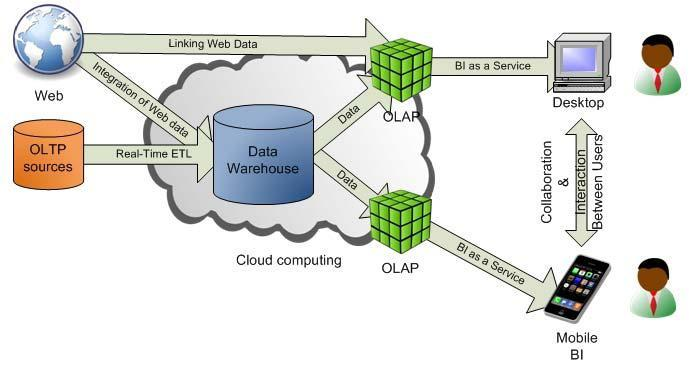
\includegraphics[width=0.6\textwidth]{./04-figuras/figura-03}
    \label{fig:ilustfig03}
\end{figure}
\vspace*{-0,9cm}
{\raggedright \fonte{Dispon\'{i}vel em: Portal (www.devmedia.com.br), Processo de Cria\c{c}\~{a}o e Exposi\c{c}\~{a}o, dispon\'{i}vel em: <https://www.devmedia.com.br/business-intelligence-2-0-conceitos-componentes-e-arquitetura/28899>, acessado em 5 jun de 2020.}}\\

Na figura acima nota-se que o BI 2.0 extrai dados n\~{a}o somente de um DW, mas sim de dados on-line e em tempo real com o aux\'{i}lio do OLTP (On-line Transaction Processing) e do Real Time ETL (Processo ETL em tempo real).

A seguir uma breve explica\c{c}\~{a}o sobre cada um de seus componentes. O bom est\'{a} ciente de que al\'{e}m das fontes de dados tradicionais, ou seja, transa\c{c}\~{a}o de dados, as fontes de dados de BI est\~{a}o evoluindo para incluir at\'{e} mesmo os mensagens enviadas por intranets empresariais e perfis pessoais de funcion\'{a}rios e clientes da web. Os dispositivos m\'{o}veis e outros dados do sensor tamb\'{e}m s\~{a}o adicionados \`{a}s fontes de dados. Contudo, muitas dessas fontes de dados n\~{a}o s\~{a}o estruturadas. Para isto precisamos entender as tecnologias:

\begin{itemize}

    \item Web 2.0: Novas pr\'{a}ticas e abordagens da web com conteúdo dinâmicos e ass\'{i}ncronos\index{NewR}\footnote{Ass\'{i}ncronos: na \'{a}rea da tecnologia da informa\c{c}\~{a}o, a comunica\c{c}\~{a}o ass\'{i}ncrona \'{e} a transmiss\~{a}o de dados, geralmente sem o uso de um sinal de rel\'{o}gio externo, onde os dados podem ser transmitidos intermitentemente em um fluxo est\'{a}vel.} que possibilitam os usu\'{a}rios interagirem com a p\'{a}gina e com outros usu\'{a}rios, ex: Redes Sociais;
    
    \item OLTP (\textit{Online Transaction Processing}):, ou seja, processamento de transa\c{c}\~{o}es em tempo real. S\~{a}o sistemas que registram as transa\c{c}\~{o}es, como, por exemplo, os ERPs (\textit{Enterprise Resource Planning});
    
    \item \textit{Real Time ETL}: Processo de extra\c{c}\~{a}o, transforma\c{c}\~{a}o e carga de dados em tempo real. Basicamente falando \'{e} uma forma de integrar os dados em tempo real, podendo ser feitos por intervalos de lotes em curto espa\c{c}o de tempo ou dependendo do segmento feito apenas algumas vezes ao dia;
    
    \item \textit{Data Warehouse}: Grande banco de dados ou armaz\'{e}m de dados, respons\'{a}vel pelo armazenamento de altos volumes de dados, ou seja, os dados brutos de uma organiza\c{c}\~{a}o; 
    
    \item \textit{Data Mart}: Reposit\'{o}rio de dados, subdivis\~{a}o de um DW, tamb\'{e}m respons\'{a}vel pelo armazenamento de dados, por\'{e}m mais espec\'{i}ficos e em menor escala;
    
    \item OLAP: An\'{a}lise e processamento on-line de dados, conhecidos tamb\'{e}m como cubos decis\'{o}rios, local onde os dados s\~{a}o analisados e processados gerando informa\c{c}\~{o}es essenciais ao neg\'{o}cio; 
    
    \item \textit{Cloud Computing}: Que se refere a computa\c{c}\~{a}o nas nuvens e tem como base a utiliza\c{c}\~{a}o da mem\'{o}ria e das capacidades de armazenamento, compartilhados e interligados por meio da Internet;
    
    \item \textit{Linking Web Data}: Refere-se a dados ligados descrevendo um m\'{e}todo de publica\c{c}\~{a}o de dados estruturados que podem ser interligados baseando-se em tecnologias da web estendendo-se para compartilhar informa\c{c}\~{o}es que podem ser lidos automaticamente por computadores; 
    
    \item \textit{Integration of Web Data}: Refere-se \`{a} integra\c{c}\~{a}o de dados, essa integra\c{c}\~{a}o combina dados residentes em diferentes fontes, tendo em vista fornecer aos usu\'{a}rios uma vis\~{a}o única dos dados;
    
    \item \textit{BI as a Service}: Refere-se \`{a} arquitetura SOA\index{NewR}\footnote{SOA \textit{(Service-Oriented Architecture)}: Significa, Arquitetura Orientada a Servi\c{c}os, numa tradu\c{c}\~{a}o livre. O conceito foi proposto pela primeira vez em 1996, no artigo “Service Oriented Architectures” (abril de 1996), escrito pelos pesquisadores \textit{Roy Schulte e Yefim Natis do Gartner Group}, e \'{e} um estilo de arquitetura de software cujo princ\'{i}pio fundamental prega que as funcionalidades implementadas pelas aplica\c{c}\~{o}es devem ser disponibilizadas na forma de servi\c{c}os.}, orientado a servi\c{c}os, o que facilita a partilha e acesso de informa\c{c}\~{o}es em tempo real.

\end{itemize}

A arquitetura orientada a servi\c{c}os (SOA) abriu caminho para o BI 2.0, pois facilita o acesso em tempo real e a coleta de dados. BI 2.0 \'{e} tamb\'{e}m mais uma vis\~{a}o de web orientada para dados tradicionais de consultas e ferramentas de an\'{a}lise.

A arquitetura de uma aplica\c{c}\~{a}o de BI 2.0 difere em alguns pontos da arquitetura de uma aplica\c{c}\~{a}o de BI tradicional ou BI 1.0. A base da arquitetura foi praticamente mantida, por\'{e}m alguns componentes foram inseridos, tais como: Web 2.0, \textit{Real Time ETL}, OLTP, Redes Sociais, SaaS ou Software como um servi\c{c}o.

Levando-se em considera\c{c}\~{a}o que o objetivo do BI 2.0 \'{e} reduzir a lat\^{e}ncia, ou seja, o tempo. Torna-se necess\'{a}rio reduzir o tempo entre quando um evento ocorre e quando uma a\c{c}\~{a}o \'{e} tomada, a fim de melhorar o desempenho empresarial, esse \'{e} o foco das arquiteturas de BI 2.0. 

A arquitetura BI 2.0 abrir\'{a} uma s\'{e}rie de op\c{c}\~{o}es para a criatividade dos usu\'{a}rios de neg\'{o}cios operacionais. 

Esta pr\'{o}xima gera\c{c}\~{a}o de BI 2.0 inclui recursos de visualiza\c{c}\~{a}o que permitem aos usu\'{a}rios ver as rela\c{c}\~{o}es entre os dados, interatividade que lhes permitem manipular os dados e uma forma intuitiva de trabalho que combina com o modo com que os usu\'{a}rios de neg\'{o}cios pensam, por exemplo, em fazer perguntas novas que podem surgir. 

Ferramentas de BI 2.0 s\~{a}o mais intuitivas para os usu\'{a}rios de neg\'{o}cios do que as ferramentas tradicionais de neg\'{o}cios, software de intelig\^{e}ncia especial e planilhas.

Finalizando esta se\c{c}\~{a}o um breve comparativo do BI tradicional ou BI 1.0 com o BI 2.0, demonstra-se na quadro abaixo as principais caracter\'{i}sticas existentes entre eles.

\begin{quadro}[H]
	\begin{center}
		\caption{Comparativo: BI Tradicional verso BI 2.0.\label{qua:quadro-02}}
	    \begin{tabular}{ |p{7cm}|p{7cm}| }
			\hline
		    Características Tradicional ou BI 1.0  
		    & 
            \textit{Next Generation Business Intelligence} ou BI 2.0 
            \\
		    \hline
            Envio e apresentação de relatórios estáticos para os usuários. Relatórios orientados para impressão. Análise de relatório pós-fato devido à latência dos dados. 
            &
            Comunidades de usuários dinâmicos com colaboração ativa e compartilhamento imediato de informações, onde os usuários elaboram seus próprios relatórios. Aplicações de geração de relatórios interativos e baseados na Web 2.0. Relatórios em tempo real. 
            \\
            \hline
            Custo elevado é considerado um luxo dentro da organização. (Empresas de grande porte). 
            &
            Soluções econômicas e rentáveis disponibilizadas para as organizações como um todo. (Pequenas, Médias e Grandes empresas).
            \\
            \hline
            Gráficos com barras estáticas, e gráficos circulares segmentados. 
            &
            Visualização de dados intuitiva, dinâmica e interativa.
            \\
            \hline
            Modelo OLAP para análise. 
            &
            Modelo OLAP junto com outras alternativas inovadoras, menos complexas e de alto.
            \\
            \hline
            Instalação, upgrade e uso complexo e de alto consumo de tempo. 
            &
            Instalação, upgrade e uso simplificados.
            \\
            \hline
            Parâmetros de pesquisa predefinidos. 
            &
            Pesquisas dinâmicas ou de estilo livre permitindo a exploração de dados.
            \\
            \hline
            Dados estruturados. 
            &
            Conjunto ampliado de tipos de dados suportados, inclusive dados não estruturados e serviços XML da web.
            \\
            \hline
            Licenciamento de software por usuário. 
            &
            Licenciamento de software por servidor para um número ilimitado de usuários ou licenciamento baseado em assinatura..
            \\
            \hline
            BI para todos, na medida da necessidade da organização.
            \\
           \hline
	    \end{tabular}
	\end{center}
	\vspace*{-0,8cm}
	{\raggedright \fonte{Disponível em: <https://www.devmedia.com.br>. Acesso em: 12 ago. 2020.}}
\end{quadro}


Assim, com base na tabela acima, podemos dizer que o BI 2.0, apresenta inova\c{c}\~{o}es e novas pr\'{a}ticas que o torna mais eficaz em rela\c{c}\~{a}o ao BI tradicional, por\'{e}m aos poucos e na pr\'{a}tica, ele traz muitos questionamentos e d\'{u}vidas em rela\c{c}\~{a}o ao seu funcionamento e desempenho no dia-a-dia.

\subsection{Tend\^{e}ncias futuras}

Antes de concluirmos esta revis\~{a}o liter\'{a}ria, falaremos um poucos sobre as tend\^{e}ncias para o futuro do Business Intelligence. Entre as principais est\~{a}o: an\'{a}lises preditivas e prescritivas, intelig\^{e}ncia artificial, intelig\^{e}ncia empresarial colaborativa, seguran\c{c}a das informa\c{c}\~{o}es, gest\~{a}o de pessoas, e o monitoramento da concorr\^{e}ncia.

A An\'{a}lises Preditivas pode ser resumida como \`{a} pr\'{a}tica de extrair informa\c{c}\~{o}es relevantes pensando em prever futuras probabilidades. J\'{a} na an\'{a}lise prescritiva, a previs\~{a}o do futuro n\~{a}o \'{e} o suficiente, \'{e} preciso encontrar uma forma de constru\'{i}-lo.

A Intelig\^{e}ncia Artificial (IA), que para muitos ainda pare\c{c}a um tema de fic\c{c}\~{a}o cient\'{i}fica, est\'{a} sendo bastante usada em diversos campos da TI, e vem forte para os pr\'{o}ximos anos e ser\'{a} uma pe\c{c}a fundamental para o \textit{Business Intelligence}. O maior motivo para seu uso e a melhora de qualidade dos processos que envolvem as tomadas de decis\~{a}o das organiza\c{c}\~{o}es. Simples assim.

A Intelig\^{e}ncia Empresarial Colaborativa, \'{e} est\'{a} em um contexto em que inúmeras empresas ao redor do mundo j\'{a} chegaram \`{a} conclus\~{a}o de que para aumentar as chances de sucesso do neg\'{o}cio, \'{e} necess\'{a}rio adotar uma gest\~{a}o colaborativa e que contribua para todos os colaboradores no que diz respeito \`{a} consecu\c{c}\~{a}o dos resultados.

A Gest\~{a}o de Pessoas, \'{e} outra tend\^{e}ncia onde o BI pode ajudar a promover o conhecimento dos funcion\'{a}rios acerca dos seus processos. A ideia maior \'{e} tornar as equipes mais conscientes sobre os erros, objetivos e metas pontuais.

O monitoramento da concorr\^{e}ncia, \'{e} indispens\'{a}vel para todo e qualquer tipo de organiza\c{c}\~{a}o que queira sair na frente e estar mais alinhada \`{a}s necessidades de seu  público alvo. Nesse ponto, o \textit{Business Intelligence} \'{e} fator imprescind\'{i}vel para o entendimento dos concorrentes: isso inclui o que eles andam fazendo e o que os clientes est\~{a}o falando sobre eles.
Vale salientar que essas tend\^{e}ncias, poder\~{a}o mudar com as inova\c{c}\~{o}es no mundo complexo da TI.

\subsection{Benef\'{i}cios e aplica\c{c}\~{o}es}

De acordo com \cite{noronha-2013} : “a grande vantagem do conceito de \textit{Business Intelligence} \'{e}justamente a capacidade que o sistema possui para ‘traduzir’ os dados armazenados em uma linguagem de f\'{a}cil assimila\c{c}\~{a}o pelo corpo gerencial das empresas. Esse ambiente gerencial geralmente \'{e}caracterizado por gr\'{a}ficos que permitem a r\'{a}pida interpreta\c{c}\~{a}o de uma situa\c{c}\~{a}o”.

Logo os gestores poder\~{a}o ter acesso \`{a}s informa\c{c}\~{o}es “rapidamente” e poder\~{a}o abreviar o tempo de resposta melhorando assim os processos decis\'{o}rios. Dessa forma, a informa\c{c}\~{a}o ser\'{a} o verdadeiro capital integralizado da empresa trazendo conhecimento para as decis\~{o}es imediatas e para aquelas que vir\~{a}o no futuro.

Abaixo as vantagens do uso e aplica\c{c}\~{a}o do BI nas organiza\c{c}\~{o}es:

\begin{itemize}

    \item Incorporar os projetos de tecnologia com as metas estabelecidas pelas empresas na busca do m\'{a}ximo retorno do investimento;
    
    \item Compreender as tendências dos neg\'{o}cios, melhorando a consistência no momento de decis\~{a}o de estrat\'{e}gias e a\c{c}\~{o}es a serem tomadas;
    
    \item Facilitar a identifica\c{c}\~{a}o de riscos;
    
    \item Planejamento corporativo mais amplo;
    
    \item Facilitar o acesso e distribuir informa\c{c}\~{a}o de modo mais amplo para obter envolvimento de todos dentro da empresa;
    
    \item Oferecer dados estrat\'{e}gicos para an\'{a}lise com um m\'{i}nimo de atraso em rela\c{c}\~{a}o a uma transa\c{c}\~{a}o ou evento dentro da empresa;
    
    \item Automatiza\c{c}\~{a}o da informa\c{c}\~{a}o de mapas de indicadores, evitando procedimentos manuais e rotineiros, obtendo diminui\c{c}\~{a}o dos custos operacionais;
    
    \item Visualiza\c{c}\~{a}o dinâmica cruzada: apresenta\c{c}\~{a}o disponibilizada em v\'{a}rias perspectivas;
    
    \item Importa\c{c}\~{a}o direta de dados de outras aplica\c{c}\~{o}es (ex.: Excel, Sistemas Legados, Sistemas Sat\'{e}lites e outras bases de dados), para tratamento dessas informa\c{c}\~{o}es;
    
    \item Passagem dos dados est\'{a}ticos para informa\c{c}\~{o}es dinâmicas;
    
    \item Permite maior flexibilidade das informa\c{c}\~{o}es das diversas fontes;
    
    \item Utiliza\c{c}\~{a}o da aplica\c{c}\~{a}o por sele\c{c}\~{a}o das vari\'{a}veis de an\'{a}lise (arrastamento e/ou filtragem por um valor determinado dessa vari\'{a}vel);
    
    \item Informa\c{c}\~{a}o sempre atualizada, mediante defini\c{c}\~{a}o e parametriza\c{c}\~{a}o pr\'{e}via.
 
 \end{itemize}
 
\subsection{Ferramentas de BI}

O conjunto de solu\c{c}\~{o}es para BI multiplicou-se e a diversidade de produtos \'{e}muito grande e continua em constante evolu\c{c}\~{a}o e crescimento tecnol\'{o}gico.

\'{e}poss\'{i}vel encontrar desde pacotes pr\'{e}-configur\'{a}veis, at\'{e}ferramentas “engessadas” e inclusive solu\c{c}\~{o}es que permitem \`{a}s empresas se aventurarem no desenvolvimento de um sistema totalmente caseiro.

Estas ferramentas têm em comum a caracter\'{i}stica de facilitar a transforma\c{c}\~{a}o dos “amontoados de dados” em informa\c{c}\~{o}es de forma a auxiliar os diversos n\'{i}veis de uma empresa na tomada segura de decis\~{o}es.

A seguir s\~{a}o enumerados algumas ferramentas que auxiliam a implantar o conceito de BI:

\begin{itemize}
    \item Planilhas eletrônicas;
    \item Geradores de consultas baseadas em SQL;
    \item Sistemas de apoio \`{a} decis\~{a}o (DSS);
    \item EIS;
    \item Linguagem MDX;
    \item Ferramentas OLAP;
    \item Ferramentas KDD;
    \item Ferramentas de BAM;
    \item Ferramentas ETLs;
    \item Ferramentas metadados;
    \item Ferramentas BPM;
    \item Ferramentas \textit{Data Mining}.
\end{itemize}

\subsection{Construir e Implementar um BI}

Primeiramente deve-se identificar as reais necessidades da empresa, especialmente as das \'{a}reas de vendas e marketing e, posteriormente, das finan\c{c}as. Ou, no caso da gera\c{c}\~{a}o de indicadores de desempenho, todas as principais \'{a}reas da empresa. 

Tamb\'{e}m deve ficar claro que apesar desses projetos envolverem o uso das ferramentas e solu\c{c}\~{o}es de tecnologia da informa\c{c}\~{a}o, \'{e}importante entender que BI \'{e}um projeto de neg\'{o}cios e por isso deve estar alinhado \`{a} estrat\'{e}gia global da corpora\c{c}\~{a}
.
Contudo, trabalhar o conhecimento usando o BI \'{e}uma linha tênue e precisa estar sempre bem “presa” \`{a}s defini\c{c}\~{o}es dos processos evolutivos da empresa, conforme a figura 4, que informa os cinco passo para a crian\c{c}\~{a}o de uma solu\c{c}\~{a}o de BI, em conjunto com novas pr\'{a}ticas comerciais, em melhores maneiras de relacionamento com os clientes e em novas formas de sobrevivência visando sempre usar a intelig\^{e}̂ncia na tomada de decis\~{a}o precisa e coerente.

\begin{figure}[H]
	\vspace*{0,2cm}
    \centering
    \caption{Composi\c{c}\~{a}o do BI em cinco passos.}
    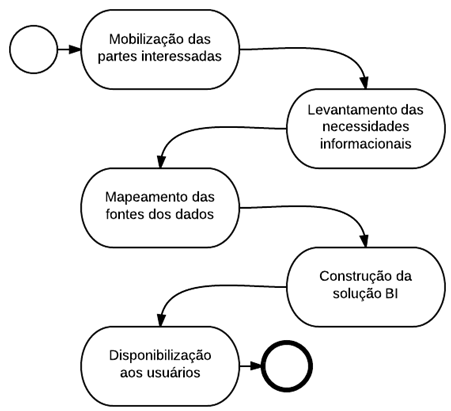
\includegraphics[width=0.6\textwidth]{./04-figuras/figura-04}
    \label{fig:ilustfig04}
\end{figure}
\vspace*{-0,9cm}
{\raggedright \fonte{Dispon\'{i}vel em: <https://canaltech.com.br>. Acesso em: 11 ago. 2020.}}\\

Essas cinco etapas constituem uma vis\~{a}o geral de todo o processo necess\'{a}rio para a completa implementa\c{c}\~{a}o e implanta\c{c}\~{a}o de uma solu\c{c}\~{a}o de BI. Todavia, a qualidade final do projeto de BI vai depender muito da aten\c{c}\~{a}o dada a cada uma dessas atividades, que descreveremos abaixo:

\begin{itemize}

    \item Mobiliza\c{c}\~{a}o das partes interessadas: para in\'{i}cio do projeto de BI, todos os \textit{stakeholders}\index{NewR}\footnote{Stakeholder: \'{e} um dos termos utilizados em diversas \'{a}reas como gest\~{a}o de projetos, comunica\c{c}\~{a}o social administra\c{c}\~{a}o e arquitetura de software referente \`{a}s partes interessadas que devem estar de acordo com as pr\'{a}ticas de governan\c{c}a corporativa executadas pela empresa.} devem ser mobilizados. Sem a participa\c{c}\~{a}o dos interessados, e principalmente do patroc\'{i}nio da alta gest\~{a}o, o BI provavelmente fracassar\'{a};
    
    \item Levantamento das necessidades informacionais: na atividade de levantamento das necessidades procuramos entender quais as informa\c{c}\~{o}es exigidas pelos gestores. Nessa etapa estamos procurando listar todas as solicita\c{c}\~{o}es sem nos preocupar, neste momento, com a exist\^{e}ncia "real" dos dados;
    
    \item Mapeamento das fontes dos dados: o mapeamento da origem dos dados \'{e} feito ap\'{o}s o levantamento das necessidades. Aqui \'{e} confrontando a viabilidade das solicita\c{c}\~{o}es efetuadas na etapa anterior. Caso afirmativo, s\~{a}o mapeadas as fontes dos dados para a posterior extra\c{c}\~{a}o na constru\c{c}\~{a}o do sistema de BI;
    
    \item Constru\c{c}\~{a}o da solu\c{c}\~{a}o BI: nessa etapa \'{e} iniciada a constru\c{c}\~{a}o propriamente dita da solu\c{c}\~{a}o. Se trata, sem dúvida alguma, da maior etapa do processo. Todas as atividades de extra\c{c}\~{a}o, qualidade dos dados, carga e teste das informa\c{c}\~{o}es s\~{a}o realizadas nesta etapa;
    
    \item Disponibiliza\c{c}\~{a}o aos usu\'{a}rios: depois de percorrido todas as etapas anteriores, chegamos, enfim \`{a} última etapa: disponibiliza\c{c}\~{a}o. Esta \'{e} uma etapa muito delicada, pois se trata do momento onde \'{e} entregue o produto de todo o esfor\c{c}o ao usu\'{a}rio final. Se a etapa de mobiliza\c{c}\~{a}o realizada no in\'{i}cio do processo tiver \^{e}xito, dificilmente teremos problemas na disponibiliza\c{c}\~{a}o. Nesta etapa, al\'{e}m de entregar a solu\c{c}\~{a}o, ser\'{a} feito toda a capacita\c{c}\~{a}o aos gestores e analistas que utilizar\~{a}o a ferramenta no dia a dia para a consulta de informa\c{c}\~{o}es de apoio \`{a}s decis\~{o}es.

\end{itemize}

Para construir um BI, primeiramente \'{e} feita a extra\c{c}\~{a}o e a an\'{a}lise dos dados da base ou das bases de dados, providos de uma gama de sistemas, os mesmos passam por um processo de transforma\c{c}\~{a}o (ETL).  

Faz-se uma limpeza deixando somente as informa\c{c}\~{o}es que ser\~{a}o úteis para a empresa. Ap\'{o}s esse processo de transforma\c{c}\~{a}o \'{e} criado os \textit{Data Marts}, ambos definidos na fase de implementa\c{c}\~{a}o, onde \'{e} feita a organiza\c{c}\~{a}o de todas as informa\c{c}\~{o}es. 

Analisando e correlacionando os dados onde posteriormente ser\~{a}o passados por outro processo de transforma\c{c}\~{a}o preparando-os para serem armazenados em um reposit\'{o}rio de dados denominado \textit{Data Warehouse}. 

Assim, quando os dados est\~{a}o no DW, todos organizados contendo somente as informa\c{c}\~{o}es relevante para o bom desenvolvimento da empresa \'{e} feita a explora\c{c}\~{a}o desses dados. 

Gerando informa\c{c}\~{o}es úteis para os usu\'{a}rios, sendo mostradas de diversas formas, atrav\'{e}s de gr\'{a}ficos, relat\'{o}rios entre outros, esse processo \'{e} feito utilizando as ferramentas OLAP, que nos oferece uma interface interativa com o usu\'{a}rio.

\section{As Principais fontes de dados}

As Fonte de dados \'{e} o local onde s\~{a}o armazenados os dados que ser\~{a}o coletados por programas de computador \textit{(softwares)} para ent\~{a}o serem transformados nas informa\c{c}\~{o}es que ir\~{a}o ajudar uma determinada \'{a}rea ou algumas \'{a}reas de neg\'{o}cio da sua empresa.

Alguns exemplos para que voc\^{e} entenda o que s\~{a}o fontes de dados:

\begin{itemize}

    \item Planilhas Eletrônicas (Excel);
    \item Banco de Dados;
    \item Arquivo CSV;
    \item Arquivo XML;
    \item Arquivos JSON;
    \item Documentos de texto (Bloco de Notas, Word, etc);
    \item Sistemas ERP;
    \item Sistemas CRM;
    \item Sociais, entre outras.
    
\end{itemize}

Conhecer e entender o que \'{e} uma fonte de dados \'{e} o ponto chave de todo o processo de implanta\c{c}\~{a}o de um BI, pois, deve-se ter certeza absoluta que os dados l\'{a} armazenados s\~{a}o \'{i}ntegros. N\~{a}o existe limite para fonte de dados, obviamente que quanto mais fontes (confi\'{a}veis) mais informa\c{c}\~{o}es e conhecimentos ser\~{a}o geradas, consequentemente mais detalhes do seu neg\'{o}cio voc\^{e} ter\'{a}. Nada adianta voc\^{e} ter 10 (dez) fontes de dados que n\~{a}o se pode confiar. 

\'{e} melhor voc\^{e} ter 2 (duas) fontes de dados com total certeza da integridade do que 10 (dez) em situa\c{c}\~{a}o duvidosa. As fontes de dados s\~{a}o a base do BI, pois s\~{a}o esses os dados que ser\~{a}o coletados e transformados em informa\c{c}\~{o}es que por sua vez ir\~{a}o gerar previs\~{o}es, an\'{a}lises, gr\'{a}ficos e relat\'{o}rios que ser\~{a}o a fonte de \textit{insights}\index{NewR}\footnote{\textit{Insight}: \'{e} o entendimento de uma causa e efeito espec\'{i}ficos dentro de um contexto espec\'{i}fico. O termo insight pode ter v\'{a}rios significados relacionados: um peda\c{c}o de informa\c{c}\~{a}o o ato ou resultado de entender a natureza interior das coisas ou de ver intuitivamente uma introspec\c{c}\~{a}o um peda\c{c}o de informa\c{c}\~{a}o; o ato ou resultado de entender a natureza interior das coisas ou de ver intuitivamente (chamado noesis em grego) uma introspec\c{c}\~{a}o; o poder da observa\c{c}\~{a}o e dedu\c{c}\~{a}o aguda , discernimento e percep\c{c}\~{a}o, chamado intelec\c{c}\~{a}o ou um entendimento de causa e efeito com base na identifica\c{c}\~{a}o de relacionamentos e comportamentos em um modelo, contexto ou cen\'{a}rio.} e a base para a tomada de decis\~{o}es de todos os colaboradores da organiza\c{c}\~{a}o.

\section{ETL (Extra\c{c}\~{a}o, Transforma\c{c}\~{a}o e Carga)}

Para \cite{dw-kimball-2013} o sistema de extra\c{c}\~{a}o, transforma\c{c}\~{a}o e carga (ETL) do ambiente DW/BI consiste em uma \'{a}rea de trabalho, estruturas de dados instanciadas e um conjunto de processos.

A extra\c{c}\~{a}o \'{e} a primeira etapa do processo de inser\c{c}\~{a}o de dados no ambiente de armaz\'{e}m de dados. Extrair significa ler e entender os dados de origem e copiar os dados necess\'{a}rios no sistema ETL para manipula\c{c}\~{a}o adicional. Neste ponto, os dados pertencem ao armaz\'{e}m de dados.

Depois que os dados s\~{a}o extra\'{i}dos para o sistema ETL, existem inúmeras transforma\c{c}\~{o}es em potencial, como limpeza dos dados (corre\c{c}\~{a}o de erros de ortografia, resolu\c{c}\~{a}o de conflitos de dom\'{i}nio, tratamento de elementos ausentes ou an\'{a}lise em formatos padr\~{a}o), combina\c{c}\~{a}o de dados de v\'{a}rias fontes e desduplicar dados. 

A etapa final do processo ETL \'{e} a estrutura\c{c}\~{a}o f\'{i}sica e o carregamento de dados nos modelos dimensionais alvo da \'{a}rea de apresenta\c{c}\~{a}o. Como a principal miss\~{a}o do sistema ETL \'{e} entregar as tabelas de dimens\~{o}es e fatos na etapa de entrega, esses subsistemas s\~{a}o cr\'{i}ticos.

Por outro lado, as tabelas de fatos s\~{a}o geralmente grandes e demoram para carregar, mas prepar\'{a}-las para a \'{a}rea de apresenta\c{c}\~{a}o \'{e} geralmente simples. 
Quando as tabelas de dimens\~{o}es e fatos em um modelo dimensional s\~{a}o atualizadas, indexadas, fornecidas com agregados apropriados e com garantia de qualidade adicional, a comunidade de neg\'{o}cios \'{e} notificada de que os novos dados foram publicados.

Ap\'{o}s validar os dados para conformidade com as regras de neg\'{o}cios definidas um-para-um e muitos-para-um, pode ser inútil dar o passo final da cria\c{c}\~{a}o de um banco de dados f\'{i}sico 3NF \textit{(Third Normal Form)}\index{NewR}\footnote{3NF (\textit{Third Normal Form} ou Terceira Forma Normal): \'{e} uma forma normal usada para normalizar um design de banco de dados para reduzir a duplica\c{c}\~{a}o de dados e garantir a integridade referencial, garantindo que: a entidade est\'{a} na segunda forma normal; Nenhum atributo n\~{a}o prim\'{a}rio (sem chave) depende transitivamente de qualquer chave, ou seja, nenhum atributo n\~{a}o prim\'{a}rio depende de outros atributos n\~{a}o primos. Todos os atributos n\~{a}o primos devem depender apenas das chaves candidatas.}, pouco antes de transformar os dados novamente em estruturas desnormalizadas para a \'{a}rea de apresenta\c{c}\~{a}o de BI.

Infelizmente, algumas iniciativas de DW/BI falharam miseravelmente, porque concentraram toda a sua energia e recursos na constru\c{c}\~{a}o de estruturas normalizadas, em vez de alocar tempo para o desenvolvimento de uma \'{a}rea de apresenta\c{c}\~{a}o dimensional que ofere\c{c}a suporte \`{a} melhor tomada de decis\~{o}es de neg\'{o}cios. 

Segundo \cite{dw-kimball-2013}, \'{e} aceit\'{a}vel criar um banco de dados normalizado para suportar os processos ETL; no entanto, esse n\~{a}o \'{e} o objetivo final. As estruturas normalizadas devem estar fora dos limites das consultas do usu\'{a}rio, pois elas derrotam os objetivos g\^{e}meos de compreensibilidade e desempenho. 

Em resumo a ETL \'{e} a respons\'{a}vel pela prepara\c{c}\~{a}o dos dados que far\~{a}o parte
do \textit{Data Warehouse} ou \textit{Data Mart}. Ela se d\'{a} basicamente em três passos: extra\c{c}\~{a}o, transforma\c{c}\~{a}o e carga de dados.

\begin{figure}[H]
	\vspace*{0,2cm}
    \centering
    \caption{ciclo de vida do ETL em todo seu processo.}
    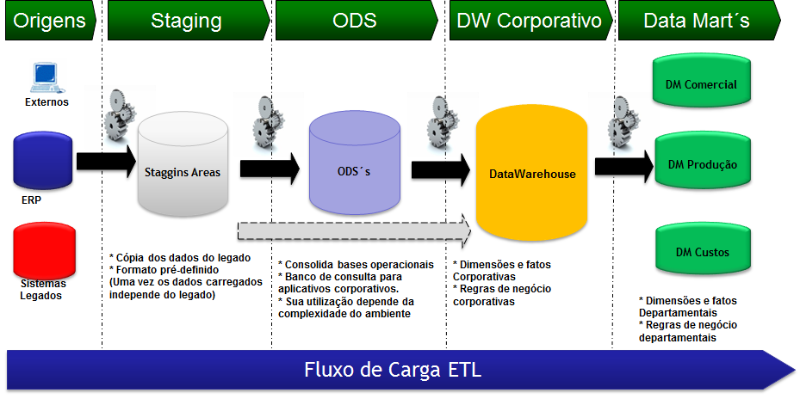
\includegraphics[width=0.6\textwidth]{./04-figuras/figura-05}
    \label{fig:ilustfig05}
\end{figure}
\vspace*{-0,9cm}
{\raggedright \fonte{Dispon\'{i}vel em: <https://https://www.igti.com.br>. Acesso em: 13 ago. 2020.}}\\

\section{\textit{Data Warehouse}}

O \textit{Data Warehouse} conforme \cite{si-inmon-1997} \'{e} o ponto central da arquitetura de processamento de informa\c{c}\~{o}es para sistemas de apoio \'{a} decis\~{a}o (SAD), visto que suportam o processamento informacional atrav\'{e}s de um alicerce s\'{o}lido de integra\c{c}\~{a}o de dados corporativos e hist\'{o}ricos para a realiza\c{c}\~{a}o de an\'{a}lises gerenciais.

De acordo com \cite{dw-kimball-2013}, um bom DW pode aliviar os sistemas de origem de grande parte da responsabilidade de representar o passado.

Segundo \cite{si-inmon-1997}, \textit{Data Warehouse} pode ser definido como uma cole\c{c}\~{a}o de dados orientados a assuntos, sendo eles integrados, n\~{a}o vol\'{a}teis e vari\'{a}veis em rela\c{c}\~{a}o ao tempo para apoio ao processo gerencial de tomada de decis\~{a}o.

Esta defini\c{c}\~{a}o acadêmica tr\'{a}s caracter\'{i}sticas importantes de um DW, que s\~{a}o melhor analisadas nas pr\'{o}ximas sess\~{o}es.

\subsection{Caracter\'{i}sticas}

Nas seguintes sess\~{o}es s\~{a}o apresentadas caracter\'{i}sticas de suma importância para um \textit{Data Warehouse}.

\subsubsection{Orienta\c{c}\~{a}o por assuntos}

A primeira caracter\'{i}stica not\'{a}vel do DW \'{e}a orientada por assunto, pois conforme Machado (2000), ela significa que o DW armazena as informa\c{c}\~{o}es agrupadas por assuntos de interesse da empresa que s\~{a}o de maior importância.

Tamb\'{e}m cabe salientar que segundo Machado (2000), os projetistas de DW devem ter seu foco na modelagem dos dados e no projeto de banco de dados. Sendo que em um DW somente importam os dados que sejam importantes para a tomada decis\~{a}o.

\subsubsection{Varia\c{c}\~{a}o tempos}

Conforme \cite{si-inmon-1997}, todos os dados no DW s\~{a}o precisos em algum instante no tempo. Esta caracter\'{i}stica b\'{a}sica dos dados do DW \'{e}muito diferente das encontradas em um ambiente operacional, pois nela quando se acessa uma unidade de dados, \'{e}esperado que esta reflita valores corretos no momento do acesso.

Em virtude de os dados no DW serem corretos como em algum momento no tempo, conforme \cite{si-inmon-1997} s\~{a}o ditos que estes variam com o tempo.

A varia\c{c}\~{a}o do tempo dos dados do DW segundo \cite{si-inmon-1997}) apresentam-se de diversas maneiras. Conforme \cite{bi-machado-2018}, a primeira e a mais simples \'{e}aquela que os dados representam informa\c{c}\~{o}es sobre espa\c{c}os de tempos de cinco a dez anos.

J\'{a} a segunda maneira s\~{a}o as estruturas b\'{a}sicas, onde cada estrutura cont\'{e}m um elemento tempo. E por fim a terceira maneira em que apresenta-se s\~{a}o os dados do DW, que uma vez armazenados corretamente, n\~{a}o podem ser atualizados \cite{si-inmon-1997}).

\subsubsection{N\~{a}o volatibilidadeos}

Conforme Inmon e Hackathorn (1997), outra caracter\'{i}stica definidora do DW trata-se do mesmo n\~{a}o ser vol\'{a}til. A manipula\c{c}\~{a}o b\'{a}sica dos dados em um DW \'{e}muito mais simples do que em ambientes operacionais, pois de acordo com Machado (2000) existem apenas dois tipos de opera\c{c}\~{o}es que podem ocorrer em um DW, a carga inicial do dados e o acesso em modo de leitura

\subsubsection{Integra\c{c}\~{a}oos}

Segundo Machado (2000), esta \'{e}uma das caracter\'{i}sticas de suma importância em um DW, pois todos os seus dados possuem um alto n\'{i}vel de integra\c{c}\~{a}o.
Conforme Inmon e Hackathorn (1997), os dados ao serem movidos de um ambiente operacional orientado a aplica\c{c}\~{o}es para o DW, s\~{a}o integrados antes de serem inclu\'{i}dos no DW. Estes mesmos autores afirmam tamb\'{e}m que os dados precisam ser armazenados no DW de uma forma única, mesmo quando as aplica\c{c}\~{o}es armazenam os dados de modo diferente.

\subsection{Granularidade de dados}

Conforme \cite{si-inmon-1997}, o aspecto mais importante do projeto de um \textit{Data Warehouse} faz referência a quest\~{a}o da granularidade, pois diz respeito ao n\'{i}vel de detalhe ou de resumo contido nas unidades de dados existentes no DW. Segundo Machado (2000), quanto mais detalhe, mais baixo o n\'{i}vel de granularidade, quanto menos detalhe, mais alto o n\'{i}vel de granularidade.

O motivo no qual torna a granularidade a principal quest\~{a}o do projeto, de acordo com \cite{si-inmon-1997} est\'{a} no fato de que ela afeta profundamente o volume de dados que encontra-se no DW e, ao mesmo tempo, afeta o tipo de consulta que pode ser atendida.

Segundo \cite{si-inmon-1997}, o n\'{i}vel de granularidade exerce um profundo efeito tanto sobre as perguntas que podem ser respondidas, bem como sobre os recursos necess\'{a}rios para responder a uma pergunta.

A escolha do n\'{i}vel ou n\'{i}veis de granularidade a serem utilizados em um projeto \'{e}indispens\'{a}vel para o sucesso. O m\'{e}todo mais indicado para definir os n\'{i}veis de granularidade conforme Machado (2000) est\'{a} na utiliza\c{c}\~{a}o do bom senso e da an\'{a}lise detalhada das necessidades de informa\c{c}\~{o}es levantadas para o projeto.
	
\subsection{Modelagem multidimensional}

Esta sess\~{a}o tem como objetivo apresentar conceitos e terminologias empregadas no processo de modelagem e na sequência deste trabalho. 

\subsubsection{Dimens\~{o}es}

Quando trata-se de dimens\~{a}o, est\'{a} se referindo aos elementos que participam de um fato, assunto de neg\'{o}cio. As dimens\~{o}es determinam o contexto de um assunto de neg\'{o}cios \cite{bi-machado-2018}.

As tabelas dimensionais conforme Kimball (1998), normalmente n\~{a}o possuem atributos num\'{e}ricos, uma vez que s\~{a}o somente textuais e classificat\'{o}rias dos elementos que participam de um fato.

Uma dimens\~{a}o de acordo com Machado (2000) pode conter membros e hierarquias. Os membros s\~{a}o uma classifica\c{c}\~{a}o de dados dentro de uma dimens\~{a}o. Estes membros de uma dimens\~{a}o podem ser arranjados em uma ou mais hierarquias, que por sua vez podem conter v\'{a}rios n\'{i}veis hier\'{a}rquicos.

\subsubsection{Fatos}

Segundo \cite{dw-kimball-2013}, a tabela de fatos em um modelo dimensional armazena as medidas de desempenho resultantes dos eventos do processo de neg\'{o}cios de uma organiza\c{c}\~{a}o.

O termo fato representa uma medida de neg\'{o}cios. Imagine estar no mercado observando os produtos sendo vendidos e anotando a quantidade de unidades e a quantidade de vendas em d\'{o}lar de cada produto em cada transa\c{c}\~{a}o de venda. 

Essas medidas s\~{a}o capturadas conforme os produtos s\~{a}o digitalizados no registro, conforme ilustrado na figura abaixo.

\begin{figure}[H]
	\vspace*{0,2cm}
    \centering
    \caption{Eventos de medi\c{c}\~{a}o de processo de neg\'{o}cios se traduzem em tabela de fato}
    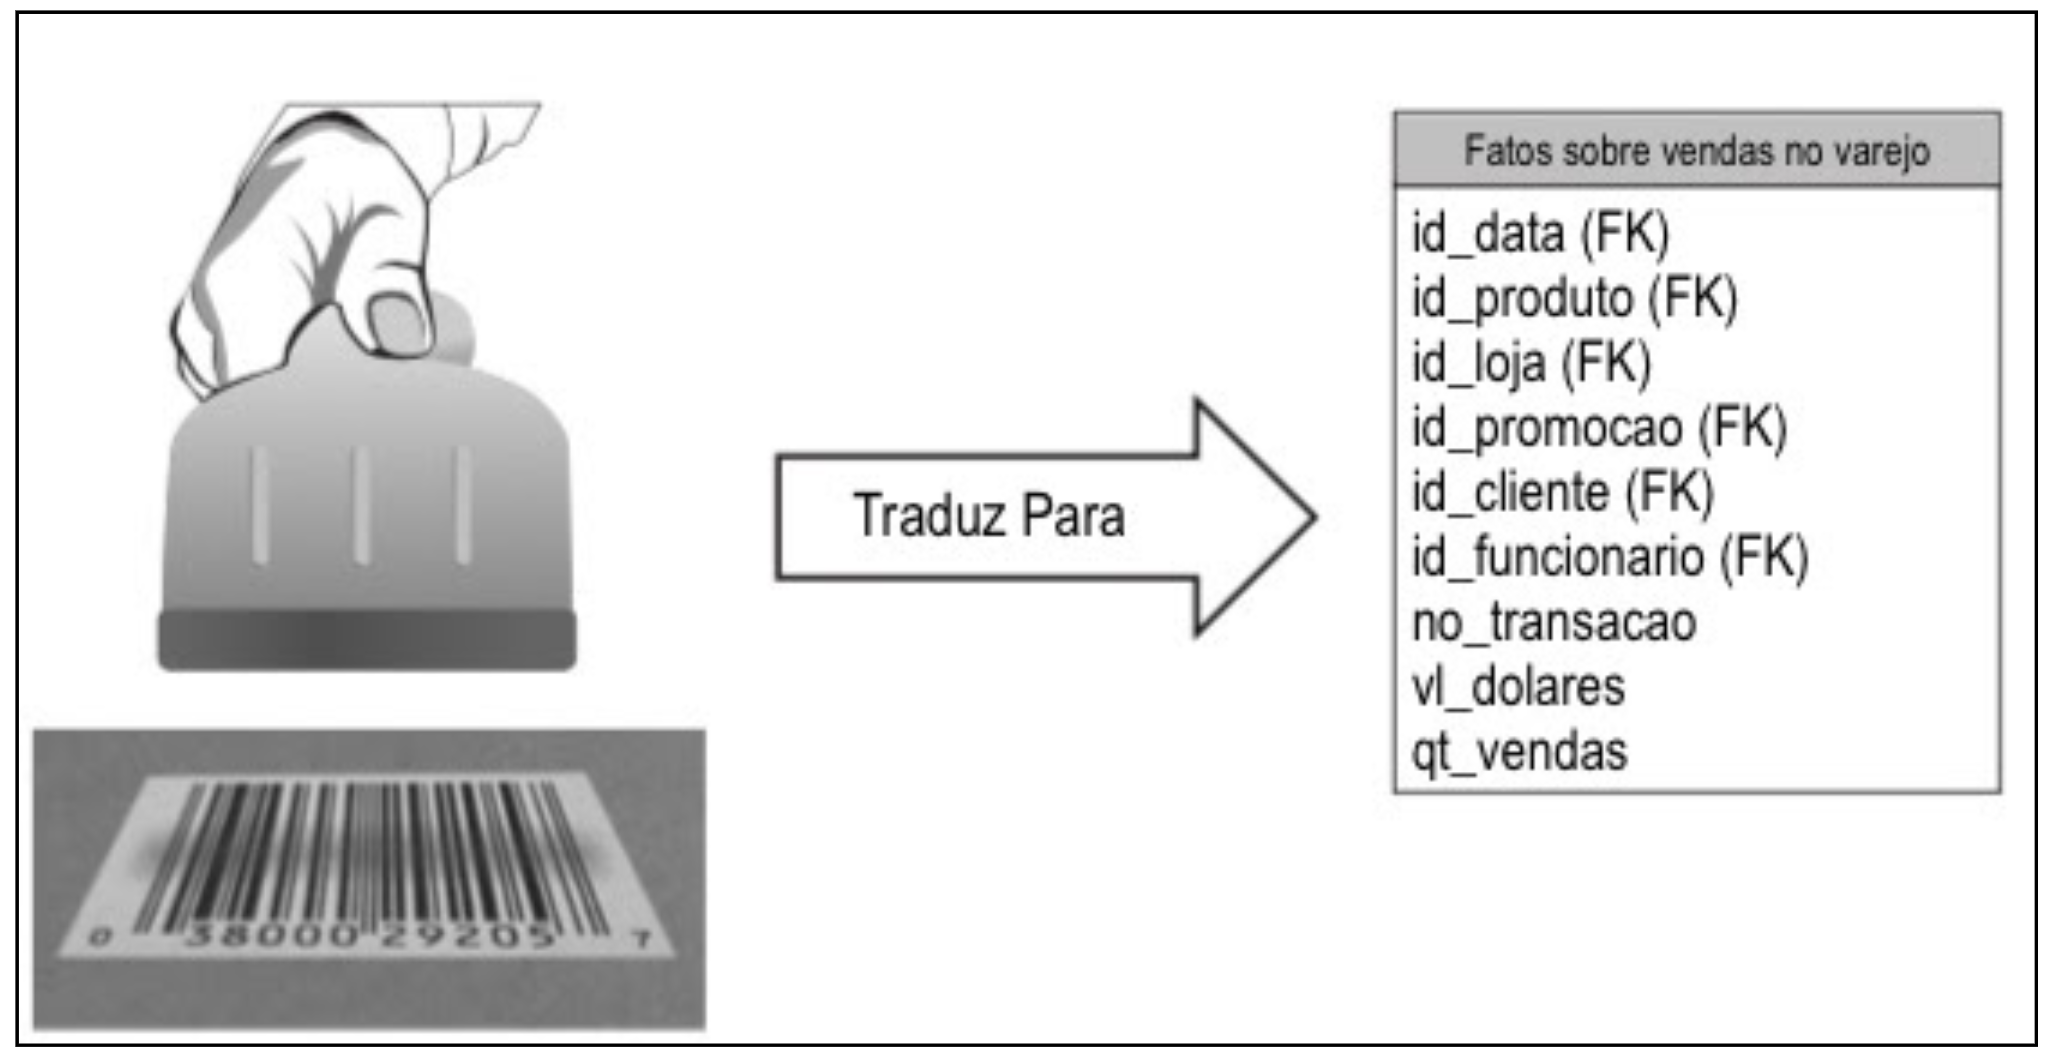
\includegraphics[width=0.6\textwidth]{./04-figuras/figura-06}
    \label{fig:ilustfig06}
\end{figure}
\vspace*{-0,9cm}
{\raggedright \fonte{adaptado de Kimball (2013)}}\\

\cite{bi-machado-2018}, conceitua que um fato trata-se de uma cole\c{c}\~{a}o de itens de dados, composta de dados de medidas e de contexto. Um fato consiste em um item de neg\'{o}cio, uma transa\c{c}\~{a}o de neg\'{o}cio ou um evento de neg\'{o}cio, nos quais se respondem as perguntas conforme figura 7. O mesmo \'{e}utilizado para verificar o processo de neg\'{o}cio de uma empresa.

De acordo com \cite{dw-kimball-1998}, tudo aquilo que reflete a evolu\c{c}\~{a}o dos neg\'{o}cios do dia-a-dia de uma institui\c{c}\~{a}o, \'{e}um fato.

\begin{figure}[H]
	\vspace*{0,2cm}
    \centering
    \caption{Fato}
    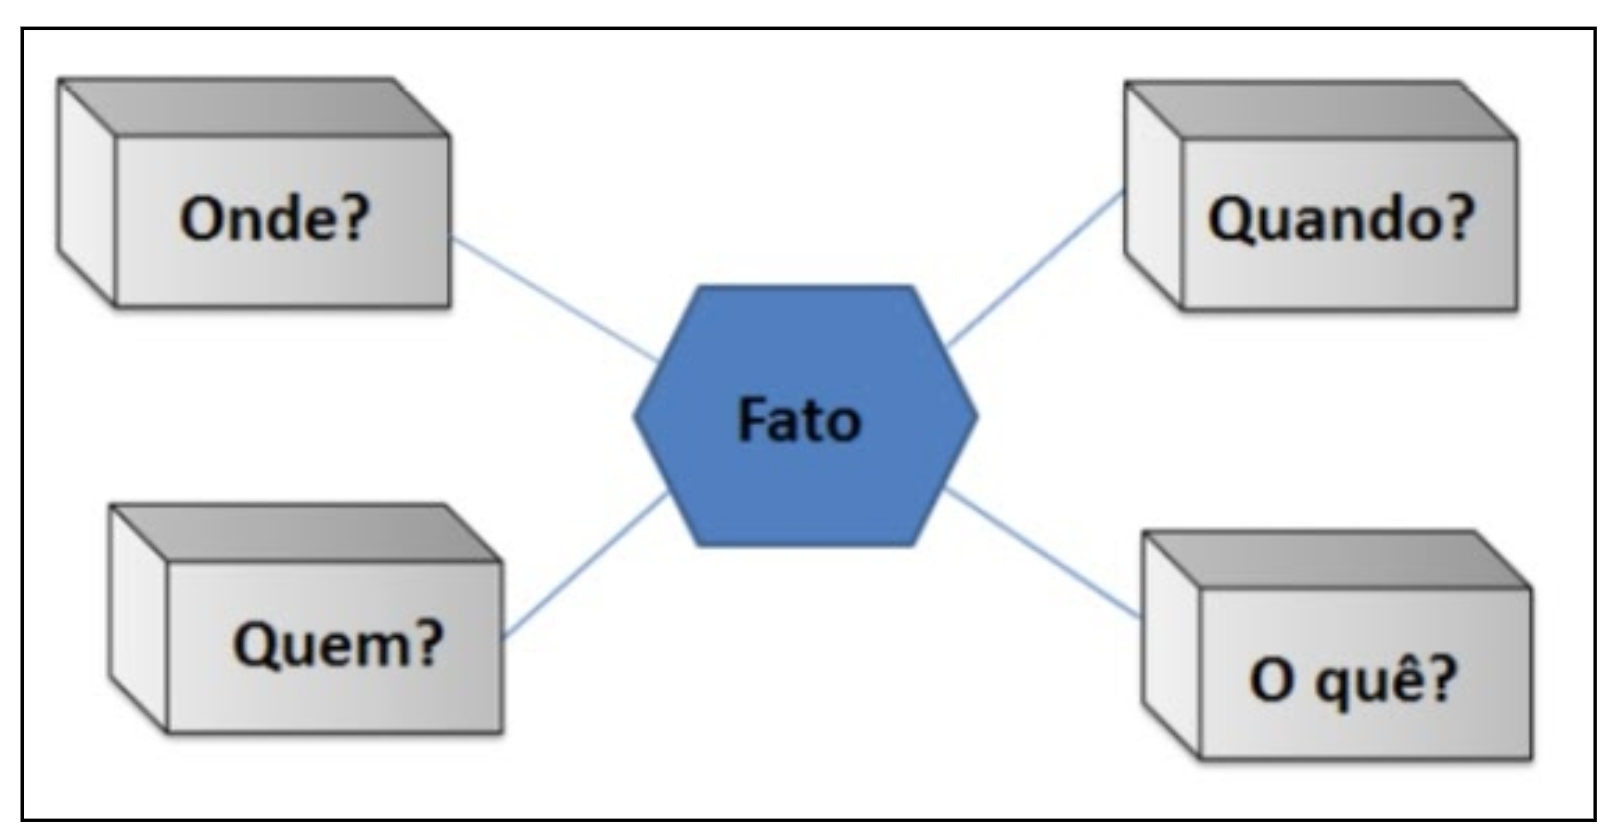
\includegraphics[width=0.6\textwidth]{./04-figuras/figura-07}
    \label{fig:ilustfig07}
\end{figure}
\vspace*{-0,9cm}
{\raggedright \fonte{adaptado de \cite{bi-machado-2018})}} \\

\subsubsection{Vari\'{a}veis}

As vari\'{a}veis ou medidas s\~{a}o os atributos num\'{e}ricos de um fato. Elas representam o desempenho de um indicador de neg\'{o}cios referente \`{a}s dimens\~{o}es que participam desse fato. Uma medida \'{e}estabelecida pela combina\c{c}\~{a}o das dimens\~{o}es que pertencem a um fato \cite{bi-machado-2018}.

\subsubsection{Opera\c{c}\~{o}es b\'{a}sicas}

Em um modelo de dados multidimensional se possu\'{i} opera\c{c}\~{o}es b\'{a}sicas de 
OLAP \textint{(On- Line Analytic Processing)}.

Conforme \cite{dw-kimball-1998}, OLAP \'{e}um termo inventado para descrever uma abordagem dimensional para o suporte \`{a} decis\~{a}o.

Estas opera\c{c}\~{o}es s\~{a}o usadas para analisar dados, sendo duas delas
:\textit{drill dow} e \textit{roll up}. Para poder-se utilizar estas opera\c{c}\~{o}es devesse fazer valer da granularidade (MACHADO, 2000).

Com a capacidade do \textit{drill down} se esta diminuindo o n\'{i}vel da granularidade, aumentando assim o n\'{i}vel de detalhes. De maneira oposta a isso, 
o \textit{roll up} aumenta o n\'{i}vel da granularidade, diminuindo desta maneira, o n\'{i}vel de detalhes das informa\c{c}\~{o}es.

\begin{figure}[H]
	\vspace*{0,2cm}
    \centering
    \caption{\textit{Drill Down} x  \textit{Roll Up}}
    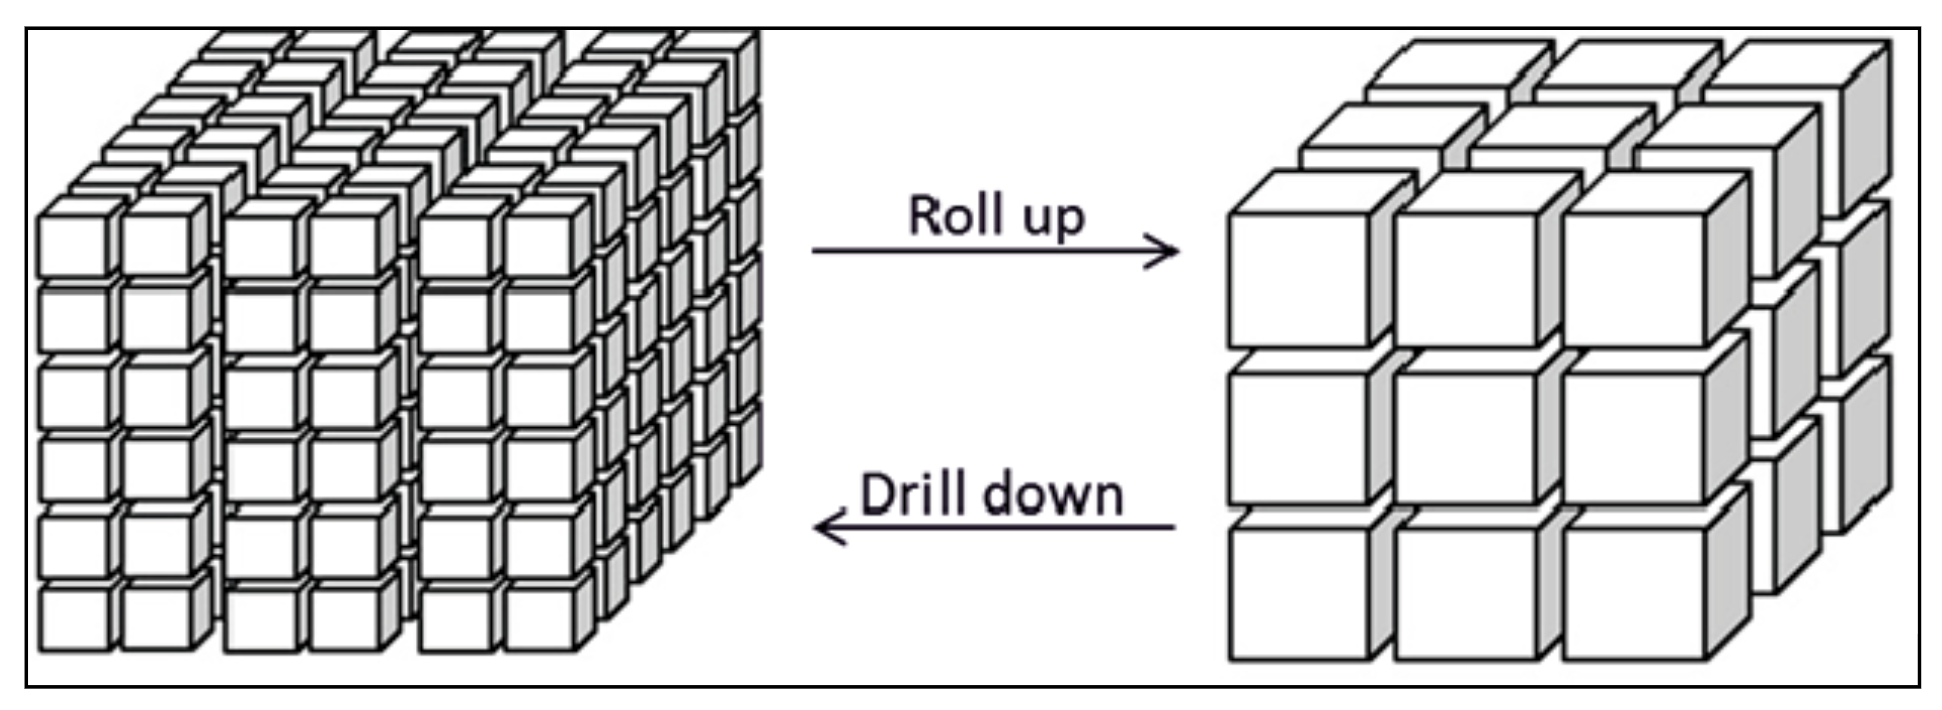
\includegraphics[width=0.6\textwidth]{./04-figuras/figura-08}
    \label{fig:ilustfig08}
\end{figure}
\vspace*{-0,9cm}
{\raggedright \fonte{Dispon\'{i}vel em: <https://(https://www.researchgate.net/figure/
Roll-up-and-Drill-down-operations-fig3-282320388>. Acesso em: 12 ago. 2020.}}\\

Portanto conforme \cite{bi-machado-2018}, estas opera\c{c}\~{o}es permitem movimentar nossa vis\~{a}o dos dados ao longo dos n\'{i}veis hier\'{a}rquicos de uma dimens\~{a}o.

\subsubsection{Modelo \textit{Star} (estrela)}

Em um modelo de dados multidimensional, a configura\c{c}\~{a}o que regula a organiza\c{c}\~{a}o dos fatos e das dimens\~{o}es para armazenamento corresponde geralmente, a um esquema em estrela \cite{bi-machado-2018}.

Este \'{e}composto por uma grande entidade central denominada tabela de fatos, e um conjunto de entidades menores denominadas tabelas de dimens\~{o}es, que por sua vez est\~{a}o organizadas ao redor da entidade central, formando assim uma estrela, conforme mostra a figura abaixo.

\begin{figure}[H]
	\vspace*{0,2cm}
    \centering
    \caption{Modelo Estrela}
    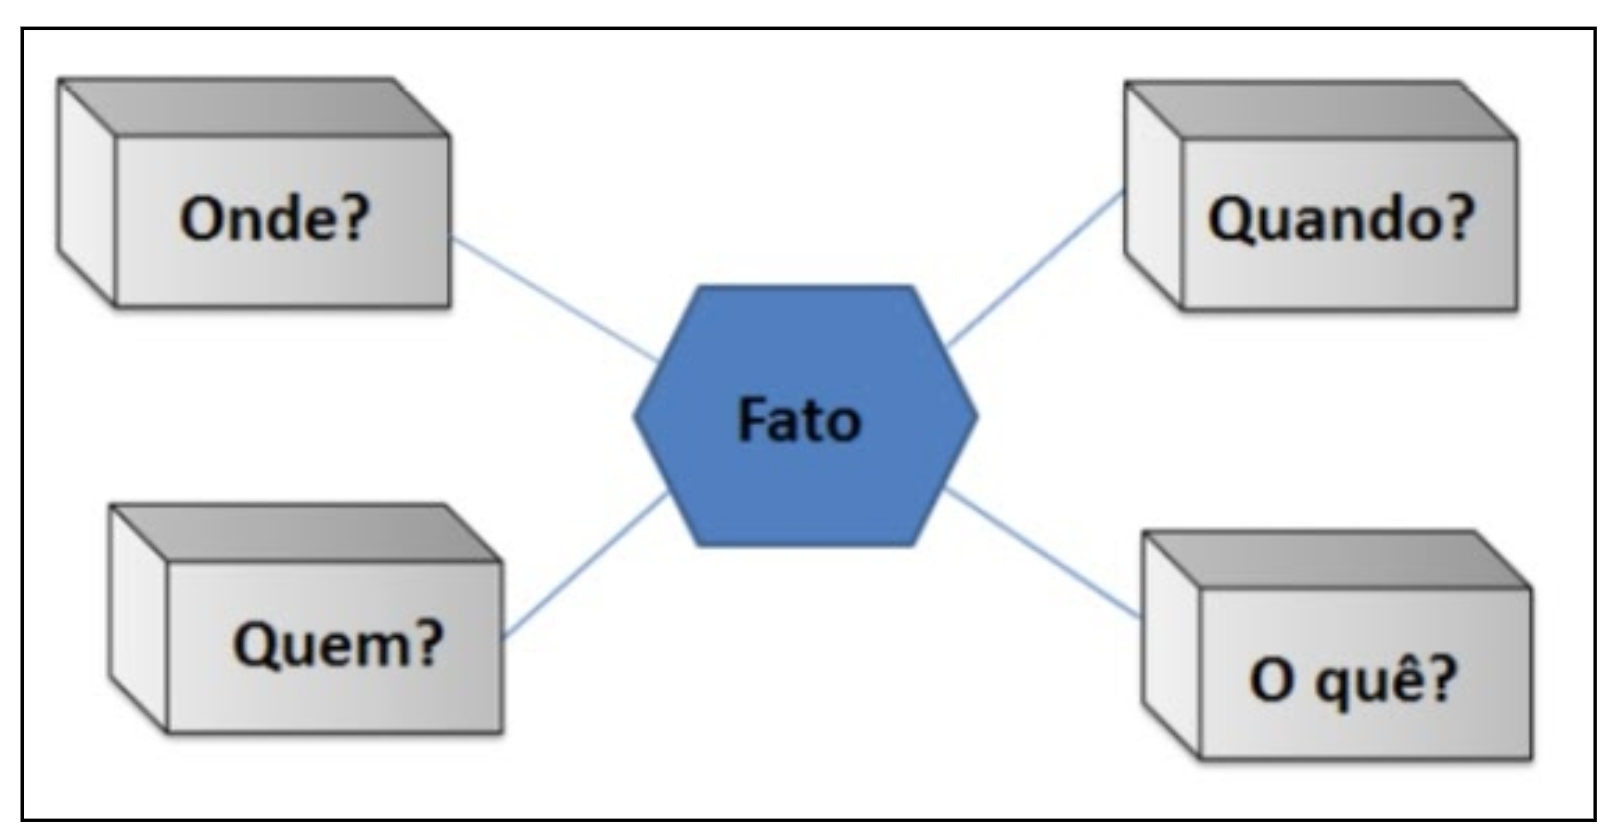
\includegraphics[width=0.6\textwidth]{./04-figuras/figura-09}
    \label{fig:ilustfig09}
\end{figure}
\vspace*{-0,9cm}
{\raggedright \fonte{adaptado de Machado (2000))}} \\

\subsubsection{Modelo \textit{Snowflake} (Floco de Neve)}

O modelo floco de neve da mesma forma que o modelo estrela possui uma entidade central denominada de fatos e um conjunto de entidades dimens\~{a}o ao seu redor formando uma estrela
.
No entanto o modelo floco de neve de acordo com \cite{bi-machado-2018}, \'{e}o resultado da decomposi\c{c}\~{a}o de uma ou mais dimens\~{o}es que possuem hierarquias entre seus membros. Conforme ilustrado na figura seguinte.
	
\begin{figure}[H]
	\vspace*{0,2cm}
    \centering
    \caption{Modelo Estrela}
    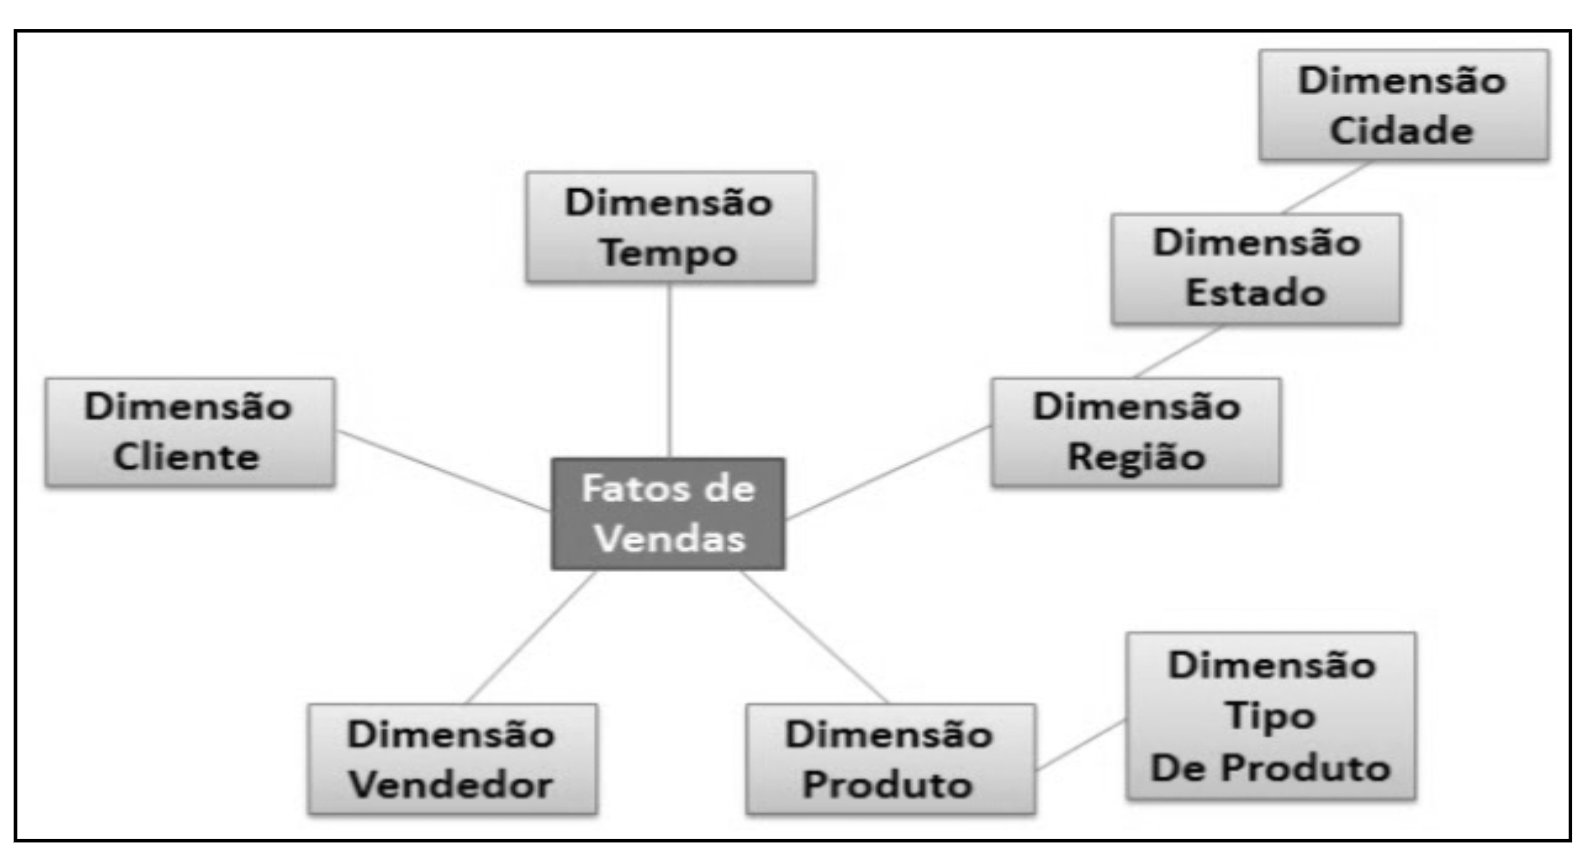
\includegraphics[width=0.6\textwidth]{./04-figuras/figura-10}
    \label{fig:ilustfig10}
\end{figure}
\vspace*{-0,9cm}
{\raggedright \fonte{adaptado de Machado (2000)}} \\

No entanto, conforme \cite{bi-machado-2018}, um DW n\~{a}o possui inclus\~{a}o de dados por meio de digita\c{c}\~{a}o, n\~{a}o necessitando assim garantir que os valores textuais sejam únicos, e nem t\~{a}o pouco se preocupar com a economia de espa\c{c}o, mas sim garantir o preceito de informa\c{c}\~{a}o r\'{a}pida.

O modelo floco de neve \'{e}esteticamente melhor para visualiza\c{c}\~{a}o de hierarquias, no entanto para se realizar consultas neste modelo s\~{a}o necess\'{a}rios mais joins, resultando assim em um gasto maior de tempo.
	
\section{\textit{Data Mart}}

Para \cite{si-inmon-1997}, um \textit{Data Mart} pode ser definido como um SGBD multidimensional que fornece uma estrutura bastante flex\'{i}vel de acesso a dados. Enquanto o DW extrai, transforma e limpa os dados dos sistemas transacionais, mantendo-os integrados em quantidades massivas e em seu n\'{i}vel mais baixo, o DM se serve destes dados, extraindo dados para um departamento ou uma \'{a}rea de neg\'{o}cio, oferecendo flexibilidade e controle ao usu\'{a}rio final, pois com o DM \'{e}poss\'{i}vel fatiar e agrupar dados de diversas maneiras.

Para \cite{bi-machado-2018} e \cite{dw-kimball-1998}, os dados do \textit{Data Mart} s\~{a}o direcionados a um departamento ou a uma \'{a}rea espec\'{i}fica do neg\'{o}cio e representam um subconjunto do DW corporativo.

O DM muitas vezes \'{e}visto como uma alternativa ao DW, pois custa menos e leva menos tempo para ser projetado e implementado. \'{e}criado para um grupo dirigido de usu\'{a}rios, normalmente um setor da empresa.

\section{KDD}

Extra\c{c}\~{a}o de conhecimento (tamb\'{e}m conhecido como processo KDD, do ingl\^{e}s 
\textit{(Knowledge Discovery in Databases)} \'{e} um processo de extra\c{c}\~{a}o de informa\c{c}\~{o}es de base de dados, que cria rela\c{c}\~{o}es de interesse que n\~{a}o s\~{a}o observadas pelo especialista no assunto, bem como auxilia a valida\c{c}\~{a}o de conhecimento extra\'{i}do.

Assim, segundo \cite{kdd-fayyad}, o KDD (\textit{Knowledge Discovery in Databases} ou Descoberta do conhecimento em Banco de Dados) \'{e} uma tentativa de solucionar o problema causado pela "era da informa\c{c}\~{a}o": sobre carga de dados.

Por\'{e}m, a difini\c{c}\~{a}o mais conhecida eo KDD, diz que ele \'{e}o processo, n\~{a}o trivial, de extra\c{c}\~{a}o de informa\c{c}\~{o}es impl\'{i}citas, previamente desconhecidas e potencialmente úteis, a partir dos dados armazenados em um banco de dados \cite{kdd-fayyad}.

O processo \'{e} n\~{a}o trivial , segundo \cite{kdd-fayyad}) j\'{a} que alguma t\'{e}cnica de busca ou infer\^{e}ncia \'{e} envolvida, ou seja, n\~{a}o \'{e} apenas um processo de computa\c{c}\~{a}o direta. 

Os padr\~{o}es descobertos devem ser v\'{a}lidos com algum grau de certeza, novos (para o sistema e de prefer\^{e}ncia tamb\'{e}m para o usu\'{a}rio), potencialmente úteis (trazer algum benef\'{i}cio) e compreens\'{i}veis (se n\~{a}o imediatamente ent\~{a}o depois da interpreta\c{c}\~{a}o).

O processo de busca de conhecimento cont\'{e}m uma s\'{e}rie de passos: sele\c{c}\~{a}o, pr\'{e}-processamento e limpeza, transforma\c{c}\~{a}o, minera\c{c}\~{a}o de dados (data mining) e interpreta\c{c}\~{a}o/avalia\c{c}\~{a}o. 

Simplificando, pode-se dizer que o processo de KDD compreende, na verdade, todo o ciclo que o dado percorre at\'{e} se transformar em informa\c{c}\~{a}o, conforme pode ser visto na figura abaixo.

\begin{figure}[H]
	\vspace*{0,2cm}
    \centering
    \caption{Ciclo dos dados em um KDD}
    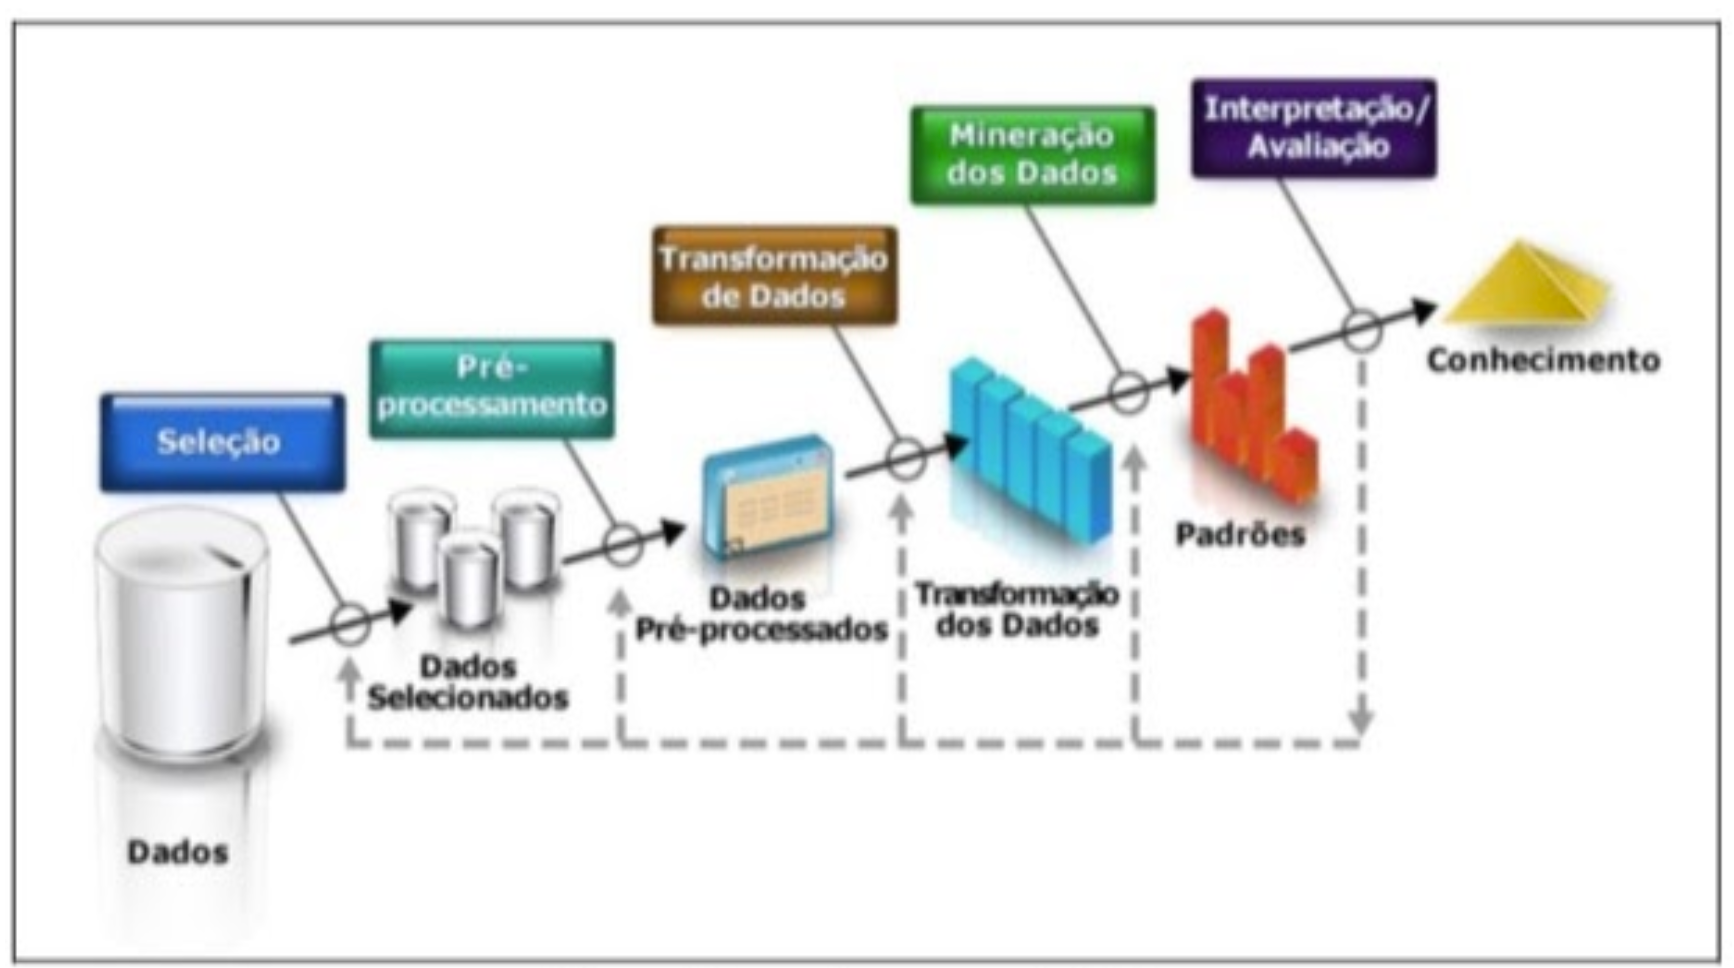
\includegraphics[width=0.6\textwidth]{./04-figuras/figura-11}
    \label{fig:ilustfig11}
\end{figure}
\vspace*{-0,9cm}
{\raggedright \fonte{adaptado de \cite{kdd-fayyad}}} \\

Suas caracter\'{i}sticas s\~{a}o:

\begin{itemize}

    \item N\~{a}o trivial j\'{a} que alguma t\'{e}cnica de busca ou infer\^{ê}ncia \'{e}envolvida (n\~{a}o \'{e}apenas um processo de computa\c{c}\~{a}o direta);
    
    \item Os padr\~{o}es descobertos devem ser v\'{a}lidos com algum grau de certeza, novos, trazer algum benef\'{i}cio e serem compreens\'{i}veis (se n\~{a}o imediatamente ent\~{a}o depois da interpreta\c{c}\~{a}o.

\end{itemize}

Em nosso trabalho n\~{a}o iremos objetivar o uso dessa tecnologia, pois, n\~{a}o \'{e} a nosso inten\c{c}\~{a}o, mas, foi preciso informar da sua exist\^{e}ncia nesse t\'{o}pico para que haja um aprofundamento te\'{o}rico de tudo que envolve o mundo do BI. 

O processo \'{e} iterativo e, embora apresente uma defini\c{c}\~{a}o semelhante tamb\'{e}m ao minera\c{c}\~{a}o de dados, deve ser composto de uma s\'{e}rie de etapas sequenciais, podendo haver retorno a etapas anteriores, isto \'{e}, as descobertas realizadas (ou a falta delas).

Eventualmente, este processo conduz a novas hip\'{o}teses e descobertas. Neste caso, o usu\'{a}rio pode decidir pela retomada dos processos de minera\c{c}\~{a}o, ou uma nova sele\c{c}\~{a}o de atributos, por exemplo, para validar as hip\'{o}teses que surgiram ao longo do processo.

O produto esperado da extra\c{c}\~{a}o de conhecimento \'{e} uma informa\c{c}\~{a}o relevante para ser utilizada pelos tomadores de decis\~{a}o. Alguns autores, por\'{e}m, defendem o ponto de vista de que o conhecimento descoberto n\~{a}o precisa necessariamente ser incorporado a um sistema de apoio \`{a} decis\~{a}o (SAD).

\section{OLAP (Processamento Anal\'{i}tico On-line)}

O OLAP \'{e}composto por inúmeras t\'{e}cnicas e ferramentas que possibilitam a explora\c{c}\~{a}o de dados armazenados em um data warehouse, utilizando t\'{e}cnicas que permitem a visualiza\c{c}\~{a}o de v\'{a}rios dados. 

Diariamente as organiza\c{c}\~{o}es acumulam grandes quantidades de dados e o OLAP as ajuda a fazer uma an\'{a}lise mais segura e confi\'{a}vel desse grande volume de dados transformando-os em informa\c{c}\~{o}es \cite{olap-jacobson-misner-2007}.

O OLAP \'{e}composto por v\'{a}rios processos usados para criar, gerenciar e manipular os dados contido no banco de dados, o mesmo tem a fun\c{c}\~{a}o de agilizar a recupera\c{c}\~{a}o dos dados, podendo ainda executar e examinar uma grande quantidade de dados. 

Os gestores das empresas usam OLAP em qualquer setor da organiza\c{c}\~{a}o, pois lhes proporciona realizar an\'{a}lises comparativas para auxili\'{a}-los nas decis\~{o}es tomadas no dia-a-dia  \cite{olap-jacobson-misner-2007}.

Os sistemas OLAP s\~{a}o conhecidos por representar algumas caracter\'{i}sticas com:

\begin{itemize}
    
    \item Oferece aos usu\'{a}rios uma resposta \`{a}s suas consultas com mais rapidez. Apresenta relat\'{o}rios que antes eram dif\'{i}ceis de analisar devida sua complexidade de uma forma mais f\'{a}cil, simples de entender.
    
    \item O OLAP oferece ferramentas para que os usu\'{a}rios possam criar seus pr\'{o}prios relat\'{o}rios, com isso poder\'{a} analisar como anda o desenvolvimento das empresas de uma forma mais r\'{a}pida e flex\'{i}vel; \cite{bi-larson-2006};
    
    \item Oferece uma forma interativa com o usu\'{a}rio durante a disponibiliza\c{c}\~{a}o das informa\c{c}\~{o}es;
    
    \item Permite que haja uma repeti\c{c}\~{a}o de dados para melhorar as consultas;
    Permite que se fa\c{c}am c\'{a}lculos com uma complexidade alta e uma visualiza\c{c}\~{a}o desses c\'{a}lculos em diversas dimens\~{o}es; e;
    
    \item Permite que se fa\c{c}am ajustes para que as consultas se tornem mais segura, para que a partir desses resultados se possam concluir analises de tend\^{e}̂ncias.

\end{itemize}

Uma organiza\c{c}\~{a}o, seja p\'{u} blica ou privada que usa OLAP ter\'{a} um desempenho melhor diante das concorrentes, pois com o uso dessa t\'{e}cnica pode trazer informa\c{c}\~{o}es com mais rapidez, da melhor forma para seu entendimento e tudo de uma forma bem interativa. 

Hoje no ambiente competitivo globalizado o que vale \'{e}ter informa\c{c}\~{a}o e estar sempre informado do que esta acontecendo no mundo, mas, principalmente, dentro de sua pr\'{o}pria empresa e essa t\'{e}cnica possibilita que todos os membros fiquem integrados do que acontece na organiza\c{c}\~{a}o de forma simples, r\'{a}pida e interativa \cite{olap-jacobson-misner-2007}.

Segundo \cite{dw-kimball-2013} o mesmo, classifica os sistemas OLAP em ROLAP, MOLAP, HOLAP E DOLAP, essas ferramentas possibilitam diferentes formas de organizar os dados antes de apresent\'{a}-los ao usu\'{a}rio final.

A ROLAP \'{e}utilizada nas an\'{a}lises mais explorat\'{o}rias dos dados, sendo bastante utilizada pela \'{a}rea de marketing. 

Quanto \`{a} ferramenta MOLAP, permite an\'{a}lises mais simples e r\'{a}pidas, mas, tamb\'{e}m, apresenta limita\c{c}\~{a}o de tamanho, tendo estrutura similar ao de uma planilha, com linhas e colunas. \cite{olap-microsoft-2020}.

A HOLAP \'{e}o resultado da combina\c{c}\~{a}o entre as ferramentas MOLAP e ROLAP, extraindo o que h\'{a} de melhor das duas. \cite{olap-microsoft-2020}.

As ferramentas DOLAP \textit{(Desktop Online Analytical Processing)} disparam uma instru\c{c}\~{a}o
SQL \textit{(Structure Query Language)} de computador simples, configurado como cliente, com um servidor de dados que retorna um microcubo de informa\c{c}\~{o}es a serem analisadas no cliente, permitindo o processamento da m\'{a}quina cliente, sem problemas de tr\'{a}fego de rede e nem problemas de escalabilidade. 

Por\'{e}m existe uma desvantagem neste processo, o microcubo n\~{a}o deve ser muito grande para que n\~{a}o haja uma perda de largura de banda \cite{olap-microsoft-2020}.

\subsection{Tipos de opera\c{c}\~{a}o sobre OLAP}

Segundo \cite{olap-ballard-2006}, as principais opera\c{c}\~{o}es utilizadas nas ferramentas OLAP s\~{a}o : \textit{Drill Across, Drill Down, Drill Up, Drill Throught, Alertas, Ranking, Filtros, Sorts, Breaks, Slice and Dice e o pivot}.

\begin{itemize}

    \item \textit{Drill Across}: ocorre quando o usu\'{a}rio atravessa um n\'{i}vel intermedi\'{a}rio numa mesma dimens\~{a}o. Ex: Ele executa um Drill Across quando h\'{a} uma altera\c{c}\~{a}o de ano para mês diretamente;

    \item \textit{Drill Down}: ocorre quando o n\'{i}vel de detalhes da informa\c{c}\~{a}o sofre um aumento;
    
    \item \textit{Drill Up}: ocorre quando o usu\'{a}rio diminui o n\'{i}vel de detalhes da informa\c{c}\~{a}o, \'{e}o contrario do Drill Down;
    
    \item \textit{Drill Throught}: ocorre quando o usu\'{a}rio muda a informa\c{c}\~{a}o de dimens\~{a}o. Ex: Est\'{a}s na dimens\~{a}o tempo e no pr\'{o}ximo passo est\'{a}s analisando a informa\c{c}\~{a}o por regi\~{a}o (outra dimens\~{a}o);
    
    \item Alertas: servem para informar sobre as situa\c{c}\~{o}es importantes e mostrar os valores mediante as condi\c{c}\~{o}es;
    
    \item \textit{Ranking}: possibilita juntar todos os resultados por ordem decrescente ou crescente, baseando-se em objetos num\'{e}ricos conhecidos como as \textit{Measures}; Filtros: d\~{a}o as permiss\~{o}es para os usu\'{a}rios aperfei\c{c}oarem, as pesquisas (Query) solicitadas por mais de uma vez, como se fossem filtros de informa\c{c}\~{o}es;
    
    \item \textit{Sorts}: serve para ordenar as informa\c{c}\~{o}es de forma crescente ou decrescente, de acordo com a escolha do usu\'{a}rio;
    
    \item \textit{Breaks}: serve para agrupar as informa\c{c}\~{o}es em blocos. Exemplo: O usu\'{a}rio que ver as informa\c{c}\~{o}es por cidades, ent\~{a}o ele executou um break. Ap\'{o}s esta a\c{c}\~{a}o ter sido executada, as informa\c{c}\~{o}es estar\~{a}o agrupadas por cidades;
    
    \item \textit{Slice and Dice}: como o OLAP gera ou recupera um micro-cubo, o Slice and Dice t\^{e}̂m a responsabilidade de fazer altera\c{c}\~{a}o na posi\c{c}\~{a}o de uma informa\c{c}\~{a}o, alterar linhas e colunas para facilitar a compreens\~{a}o dos usu\'{a}rios e girar o cubo sempre que tiver necessidade, esse recurso faz parte das principais caracter\'{i}sticas da ferramenta;
    
    \item \textit{Pivot}: Permite a troca de linhas por colunas em uma tabela ou modifica\c{c}\~{a}o da posi\c{c}\~{a}o das dimens\~{o}es em um gr\'{a}fico. Ou seja, \'{e} o ângulo pelo qual os dados s\~{a}o visualizados.
    
\end{itemize}

Conforme \cite{dw-kimball-2013}, o OLAP \'{e}uma tecnologia de banco de dados que foi otimizada para consulta e relat\'{o}rio, em vez de processamento de transa\c{c}\~{o}es. Os dados de origem do OLAP s\~{a}o bancos de dado OLTP\textit{(Online Transactional Processing)} que s\~{a}o comumente armazenados em um \textit{Data Warehouse}.

Os dados OLAP s\~{a}o originados a partir desses dados hist\'{o}ricos, e integrados em estruturas que permitem an\'{a}lise sofisticada, sendo organizados hierarquicamente e armazenados em cubos em vez de tabelas. Esta tecnologia \'{e}organiza de forma f\'{a}cil as estruturas multidimensionais para agilizar o acesso aos dados a serem analisados. 

Logo, s\~{a}o a base dos relat\'{o}rios de tabelas ou gr\'{a}ficos dinâmicos, e a exibi\c{c}\~{a}o de resumos de alto n\'{i}vel, bem como a exibi\c{c}\~{a}o de resultados detalhistas.

\subsection{Os componentes do OLAP}

Os tipos de dados que constituem os bancos de dados OLAP s\~{a}o as medidas e as dimens\~{o}es, sendo as medidas, os dados num\'{e}ricos, ou seja, as quantidades e m\'{e}dias que você usa para tomar decis\~{o}es comerciais, e as dimens\~{o}es s\~{a}o as categorias que voc\^{e}̂ usa para organizar essas medidas.

Os bancos de dados OLAP auxiliam na organiza\c{c}\~{a}o dos dados por muitos n\'{i}veis de detalhe, utilizando algumas categorias que ser\~{a}o descritas a seguir \cite{olap-microsoft-2020}:

\begin{itemize}

    \item Cubo: s\~{a}o formas de dados que ajudam na realiza\c{c}\~{a}o de an\'{a}lises, sem eles n\~{a}o seria poss\'{i}vel realizar an\'{a}lises de dados em diversas dimens\~{o}es. Eles possibilitam combinar o tempo, a geografia e os produtos com números de vendas de forma r\'{a}pida, eficiente e resumida;
    
    \item Medida: s\~{a}o todos os valores num\'{e}ricos encontrados na regi\~{a}o central de um cubo, como por exemplo, as vendas, os lucros, as receitas e os custos, todos processados, agregados e analisados;
    
    \item Membro: \'{e} caracterizado por objetos que podem desempenhar um ou mais impacto de dados em uma hierarquia; Membro calculado: o valor de um membro \'{e}calculado enquanto esta ocorrendo uma execu\c{c}\~{a}o por meio de uma express\~{a}o. O valor de um membro calculado pode ser originado do valor de outro membro;
    
    \item Dimens\~{a}o: \'{e} composta por uma ou mais hierarquias organizadas de n\'{i}veis em um cubo de uma forma que o usu\'{a}rio possa entender e assim us\'{a}-las para fazer an\'{a}lise de dados;
    
    \item Hierarquia: \'{e}uma forma de ordena\c{c}\~{a}o em diferentes n\'{i}veis organizando os membros de uma dimens\~{a}o de forma que cada membro tenha um possa ter um membro pai e zero ou at\'{e}mais membros filho. De acordo com a hierarquia o membro filho \'{e}inferior ao membro atual, j\'{a} o pai est\'{a} em um n\'{i}vel superior relacionado diretamente ao membro atual. O valor pai \'{e}no gera consolidado aos valores de todos os seus filhos;
    
    \item N\'{i}vel: em um processo hier\'{a}rquico, os dados podem ser ordenados em n\'{i}veis de detalhe inferiores e superiores, como por exemplo, Ano, Semestre, Trimestre, Mês e Dia em uma hierarquia Tempo.

\end{itemize}

\subsection{As Aplica\c{c}\~{o}es do OLAP}

O OLAP \'{e}caracterizado por ser diversificado, podendo ser aplicado em diversos setores de uma organiza\c{c}\~{a}o como no setor de \cite{olap-microsoft-2020}:

\begin{itemize}

    \item Nas finan\c{c}as: nesse setor com o uso de OLAP poder\'{a} ser realizada uma analise de balan\c{c}o geral da empresa, fazer um or\c{c}amento, fluxo de caixa da empresa, contas \`{a} receber;
    \item Nas vendas: pode ser feita uma an\'{a}lise das vendas escolhendo a regi\~{a}o, os produtos que mais foram vendidos nesta regi\~{a}o, o vendedor respons\'{a}vel pelas vendas, entre outros dados;
    \item No \textit{Marketing}: o OLAP possibilita que fa\c{c}a uma an\'{a}lise de mercados, lucratividade de produto, e fazer uma an\'{a}lise de pre\c{c}o ou volume;
    \item Nos Recursos Humanos: com os sistemas OLAP poder\'{a} ser feito uma an\'{a}lise de benef\'{i}cios, fazer proje\c{c}\~{a}o de sal\'{a}rios e analise de números de funcion\'{a}rios da empresa ou do setor; e;
    \item Na Manufatura: atrav\'{e}s dessa ferramenta OLAP pode-se gerenciar o estoque da empresa, os fornecedores, fazer planejamento de que produtos est\~{a}o em demanda, analisar os custos dos materiais para fabrica\c{c}\~{a}o dos produtos.

\end{itemize}

\subsection{As Ferramentas OLAP}

Os gestores das organiza\c{c}\~{o}es tem a necessidade de uma ferramenta que os auxiliem na explora\c{c}\~{a}o dos dados que forne\c{c}a informa\c{c}\~{o}es confi\'{a}veis, que de acordo com a an\'{a}lise das mesmas possam os auxiliar na tomada de decis\~{a}o. 

Para isso existem algumas ferramentas que poder\~{a}o ajuda-los nesse processo de explora\c{c}\~{a}o e analise dos dados como o \textit{Mondrian} ou textit{Schema Workbench} , que ser\'{a} tema de um t\'{o}pico especifico, e que faz parte do Pentaho.

\section{Cubo}

Segundo Carlo Vercellis \cite{dm-vercellis-2009}, o projeto de DW e \textit{data mart} s\~{a}o baseados em um paradigma multidimensional para a representa\c{c}\~{a}o de dados que fornece grandes vantagens no momento da consulta de dados, ele pode garantir tempo de resposta r\'{a}pida, mesmo em complexas consultas, enquanto no lado l\'{o}gico, as dimens\~{o}es naturalmente correspondem a crit\'{e}rios normais e facilmente entend\'{i}veis a usu\'{a}rios para realizarem suas an\'{a}lises.

A representa\c{c}\~{a}o multidimensional \'{e}baseada em um esquema em estrela que cont\'{e}m os dois tipos de tabelas de dados, as dimens\~{o}es e Fatos.

Com isso pode-se dizer que um cubo, \'{e}a estrutura multidimensional de dados que expressa a forma na qual os tipos de informa\c{c}\~{o}es se relacionam entre si. \'{e}formado pela tabela Fato e pelas tabelas de dimens\~{a}o que a circundam e representam poss\'{i}veis formas de visualizar e consultar os dados \cite{dm-vercellis-2009}.

Pode-se citar um exemplo de um cubo atrav\'{e}s de um conjunto de lojas, considerando o faturamento de um produto em um mês do ano, em uma loja.

Na existência de um cubo tridimensional, uma dimens\~{a}o representa os produtos, a outra o per\'{i}odo e outra as lojas. A figura logo abaixo,  representa o exemplo.

% figuras
\begin{figure}[H]
	\vspace*{0,2cm}
    \centering
    \caption{Cubo}
    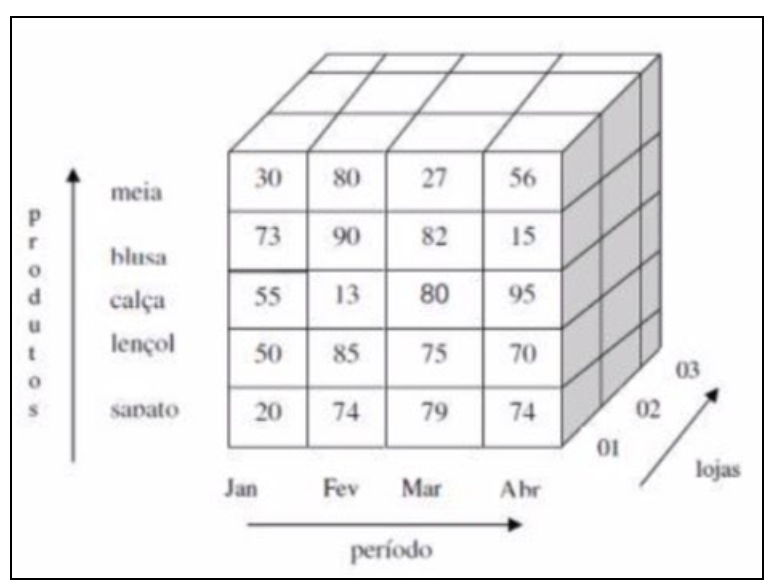
\includegraphics[width=0.6\textwidth]{./04-figuras/figura-12}
    \label{fig:ilustfig12}
\end{figure}
\vspace*{-0,9cm}
{\raggedright \fonte{\cite{dm-vercellis-2009}}} \\

\section{\textit{Data mining} (minera\c{c}\~{a}o de dados)}

Alguns profissionais da \'{a}rea de an\'{a}lise de informa\c{c}\~{a}o enfrentam problemas no processo de transformar dados que as empresas acumulam em suas transa\c{c}c\~(oo)es di\'{a}rias em informa\c{c}\~{o}es que ser\~{a}ao de grande utilidade para o desempenho dos neg\'{o}ocios. 

Assim, Segundo CORTES, o \textit{Data Mining} \'{e}um processo feito sobre enormes reposit\'{o}rios de dados como o \textit{data warehouse} buscando identificar padr\~{o}es e alguma rela\c{c}\~{a}o de consumo que n\~{a}o s\~{a}o conhecidos pela empresa e que podem ser usados na tomada de decis\~{a}o \cite{bi-cortes-2008}.

Usando o \textit{Data Mining} esse problema ser\'{a} resolvido, pois ele \'{e}um processo pelo qual se descobri informa\c{c}\~{o}es importantes para a empresa, como os padr\~{o}es, as associa\c{c}\~{o}es entre as informa\c{c}\~{o}es da base de dados, mudan\c{c}as, anomalias e as estruturas, em grandes quantidades de dados que s\~{a}o armazenados em base de dados ou outros reposit\'{o}rios de dados \cite{bi-cortes-2008}.

    %
% Documento: Metodologia
%

\chapter{METODOLOGIA}

Para a realização deste trabalho serão aplicados os conceitos estudados sobre BI com foco em na implementa\c{c}\~{a}o de um DW/BI para o 181, usando para isso o Suite Pentaho, desenvolvida pela empresa Pentaho Corporation e mantida atualmente pela Hitachi Vantara.

No desenvolvimento desta monografia foram aplicados os conceitos estudados sobre BI, tomando como base no modelo de Kimball (2013) usando como  plataforma o BI Hitachi Pentaho, conforme tópico 4.4, suite mantida atualmente pela empresa Hitachi Vantara. 

O trabalho foi construído para que, primeiramente, seja entregue ao leitor uma introdução ao BI e suas definições assim como explicar o seu conceito e uso pr\'{a}tico através da plataforma Pentaho. Uma explicação em cada uma das principais etapas do BI, posteriormente uma apresentação sobre as ferramentas escolhidas a serem estudadas, conforme tópico 4.2, e por fim uma conclusão destes casos de uso, pr\'{a}tico atr\'{a}ves de dados reais do Disque Denúncia do Estado de Alagoas.

A metodologia é baseada na pesquisa-a\c{c}\~{a}o, junto a elementos qualitativos e quantitativos, onde ser\'{a} demonstrado os processo de extração dos dados,  cria\c{c}\~{a}o de um \textit{Data Warehouse}, com consultas e cubos OLAP an\'{a}lise usando o \textit{plugin} SAIKU, \textit{Dashboard}\index{NewR}\footnote{\textit{Dashboard} ou Painel de Controle é a apresenta\c{c}\~{a}o visual das informa\c{c}ões mais importantes e necess\'{a}rias para alcan\c{c}ar um ou mais objetivos de negócio, consolidadas e ajustadas em uma tela para f\'{a}cil acompanhamento do seu negócio}, CDE, baseado no módulo consultar denúncia, ao gerar os recursos de BI necess\'{a}rios.      
    %
% Documento: Desenvolvimento
%

\chapter{DESENVOLVIMENTO}

Neste capítulo iremos utilizar \`{a}s teorias do capítulo 2 (Revis\~{a}o liter\'{a}ria) juntamente com as t\'{e}cnicas de Kimball R. e Ross, M. (2013), que se baseiam na modelagem dimensional e iremos teorizar as ferramentas de banco de dados PostgreSQL e Pentaho, para que tenhamos uma base de conhecimento s\'olida em rela\c{c}\~{a}o ao uso e funcionalidades destas ferramentas.

O objetivo deste capítulo \'{e} a implementa\c{c}\~{a}o de um BI/DW, partindo da infraestrutura b\'{a}sica, cria\c{c}\~{a}o do Banco de dados de nome: ``DW\_181'' no PostgreSQL, ETL dos dados de três meses  (janeiro, fevereiro e mar\c{c}o de 2020) de transa\c{c}\~{o}es, provindos do arquivo no formato ``.XLS'' do \textit{Microsoft Excel},  extraído do SISGOU, na op\c{c}\~{a}o consulta do disque denúncia, que ser\'{a} processada usando uma das ferramentas do suite Pentaho, o PDI (\textit{Pentaho Data Integration}).

No PDI iremos criar as transforma\c{c}\~{o}es que criaram as tabelas de dimens\~{a}o dentro do Banco de dados, al\'{e}m do PDI iremos demonstrar o uso das outras ferramentas do Pentaho como: PAC (\textit{Pentaho Administration Console}), PUC (\textit{Pentaho User Console}), PSW (\textit{Pentaho schema workbench}) e o PRD (\textit{Pentaho Report Designer}) e finalmente ap\'os os dados serem processados ser\~{a}o armazenados no PostgreSQL, SGBD relacional, onde ficar\'{a} o DW da aplica\c{c}\~{a}o de BI.

\section{Infraestrutura}

A infraestrutura utilizada neste trabalho \'{e} baseada em ferramentas de softwares gratuitos ou \textit{freeware} , da suite de BI ao SGDB relacional, para a base de dados, usamos oPostgreSQL, como dito no t\'opico anterior, juntamente com a Plataforma Pentaho na vers\~{a}o 9.0 \textit{Community} (sem custos), adquirida no site da Hitachi Vantara atualmente \'{e} detentora dos direitos da plataforma e o Java SE \textit{Runtime Environment} vers\~{a}o 1.8.0-151-b12, toda estrutura instalada localmente em um ambiente de desenvolvimento, em um notebook MacBook Pro da Apple (mem\'oria de 16 gb de ram e SSD de 1 Tb), com Sistema Operacional macOS Catalina vers\~{a}o 10.15.6.

\section{SISGOU}

O sistema de processamentos de transa\c{c}\~{o}es de onde se extraíram os dados \'{e} o SISGOU, desenvolvidos pelo equipe de TI da SSP/AL, conforme figura abaixo, nele todos os dados das denúncias s\~{a}o registrados pelos atendentes, e ou, denunciantes (via web ou aplicativo), s\~{a}o armazenados em uma base de dados em ORACLE, \'{e} os usu\'{a}rios finais têm acesso apenas pelo menus da aplica\c{c}\~{a}o, em nosso caso m\'odulo "Aplicativos", "Disque Denúncia" e "Consultar Denúncias", conforme figura abaixo.

% figuras
\begin{figure}[H]
	\vspace*{0,2cm}
    \centering
    \caption{SISGOU (Sistema de Gerenciamento Operacional Unificado}
    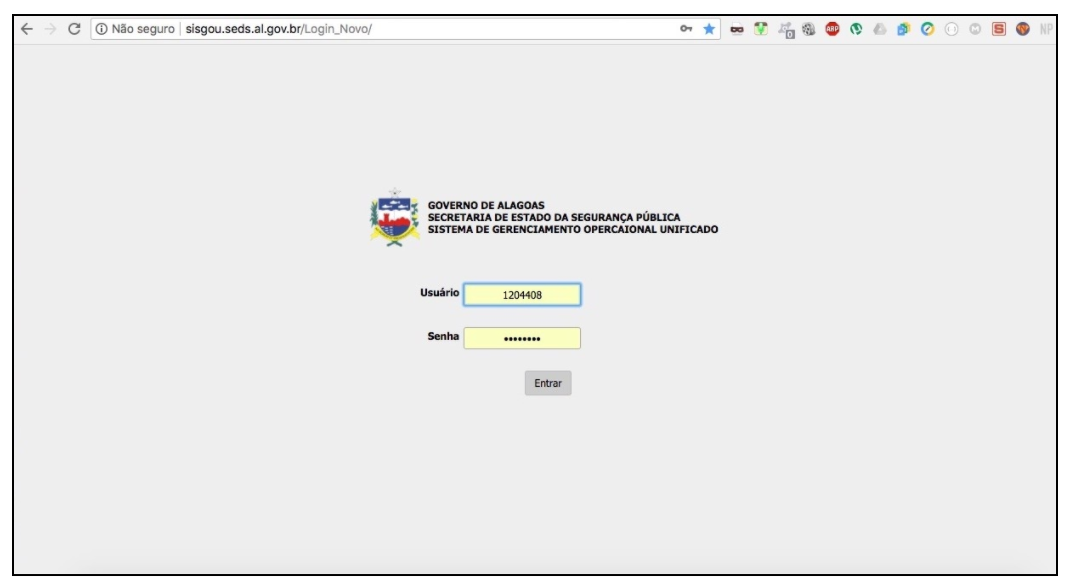
\includegraphics[width=0.6\textwidth]{./04-figuras/figura-13}
    \label{fig:ilustfig13}
\end{figure}
\vspace*{-0,9cm}
{\raggedright \fonte{Disponível em: <https://https://www.sisgou.seds.al.gov.br>. Acesso em: 13 ago. 2020.}}\\

% FERRAMENTAS

\section{Ferramentas}

% SGDB POSTGRESQL

\subsection{SGDB PostgreSQL}

O PostgreSQL \'{e} um sistema de gerenciamento de banco de dados relacional de objeto (ORDBMS) baseado no PostgreSQL, vers\~{a}o 4.2, desenvolvido no Departamento de Ciência da Computa\c{c}\~{a}o da Universidade da Calif\'ornia em \textit{Berkeley}. O PostgreSQL foi pioneiro em muitos conceitos que s\'o se tornaram disponíveis em alguns sistemas de bancos de dados comerciais muito depois.

Al\'{e}m disso, o PostgreSQL pode ser estendido pelo usu\'{a}rio de v\'{a}rias maneiras, por exemplo, adicionando tipos de dados, fun\c{c}\~{o}es, operadores, fun\c{c}\~{o}es agregadas, m\'{e}todos de índice e uma linguagens processuais. Que n\~{a}o ser\~{a}o especificados nesse trabalho.

E por causa da licen\c{c}a liberal, o PostgreSQL pode ser usado, modificado e distribuído gratuitamente por qualquer pessoa, seja para fins particulares, comerciais ou acadêmicos.

Em nosso trabalho a cria\c{c}\~{a}o, modelagem e o armazenamento dos dados do \textit{Data Warehouse} foi utilizado o PostgreSQL, vers\~{a}o 9.5, e com gerenciador administrativo o aplicativo ``pgAdmin'' vers\~{a}o 4. 

Para gerenciar o PostgreSQL, podemos fazê-lo de duas maneiras: uma por meio de uma s\'{e}rie de comandos SQL e ou atrav\'{e}s do aplicativo ``pgAdmin''. Neste trabalho enfocaremos o artifício da cria\c{c}\~{a}o do banco de dados, suas tabelas e \textit{constraints}, usando a interface gr\'{a}fica do aplicativo acima, e tamb\'{e}m atrav\'{e}s do PDI, que gera \textit{scripts} com as instru\c{c}\~{o}es para a cria\c{c}\~{a}o da tabela, atrav\'{e}s do processo de transforma\c{c}\~{a}o, criado no PDI, que ser\'{a} mencionado em um t\'opico específico.

\begin{figure}[H]
	\vspace*{0,2cm}
    \centering
    \caption{Ferramenta ``pgAdmin' vers\~{a}o 4 para o PostgreSQL}
    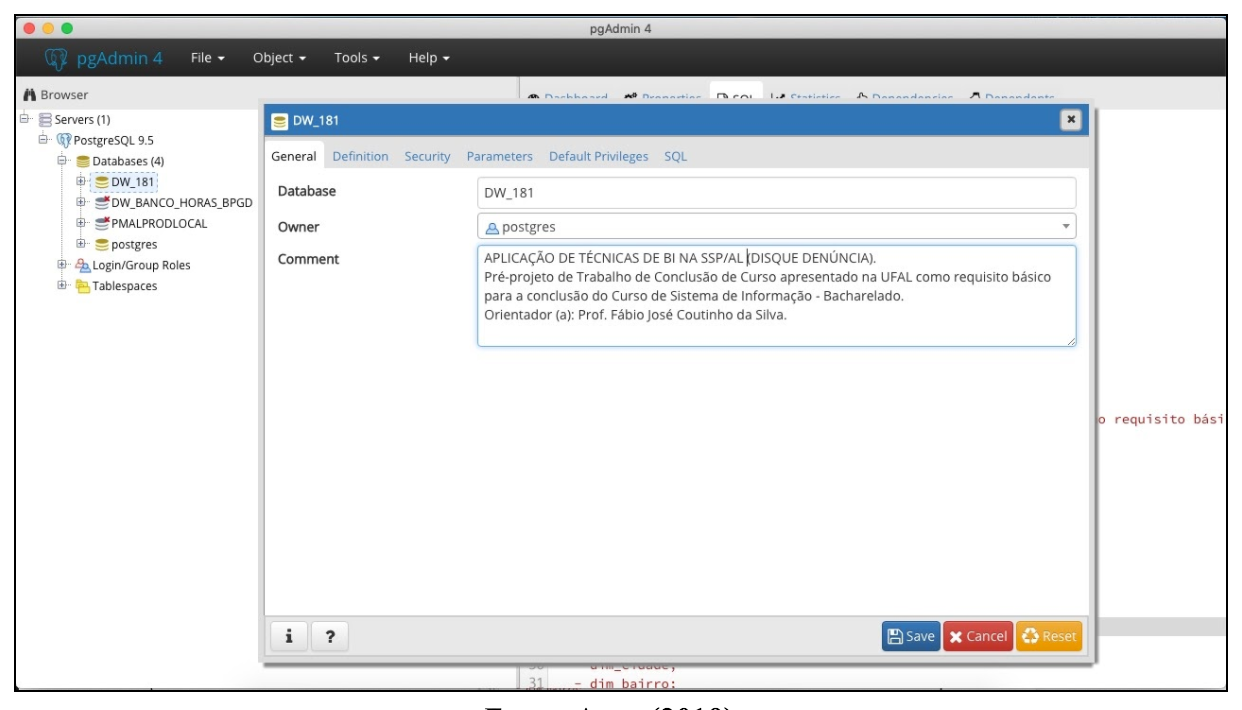
\includegraphics[width=0.6\textwidth]{./04-figuras/figura-14}
    \label{fig:ilustfig14}
\end{figure}
\vspace*{-0,9cm}
{\raggedright \fonte{Autor desta monografia, 2020.}} \\

% PENTAHO

\subsection{Plataforma Pentaho}

Outra ferramenta fundamental neste trabalho \'{e} a Plataforma de Integra\c{c}\~{a}o de Dados e An\'{a}lise Pentaho, nele iremos implementar todos os conceitos de DW/BI. Para isso precisamos conhecer um pouco sobre essa ferramenta, conforme figura abaixo.

\begin{figure}[H]
	\vspace*{0,2cm}
    \centering
    \caption{\textit{Pentaho Business Analytics Platform}}
    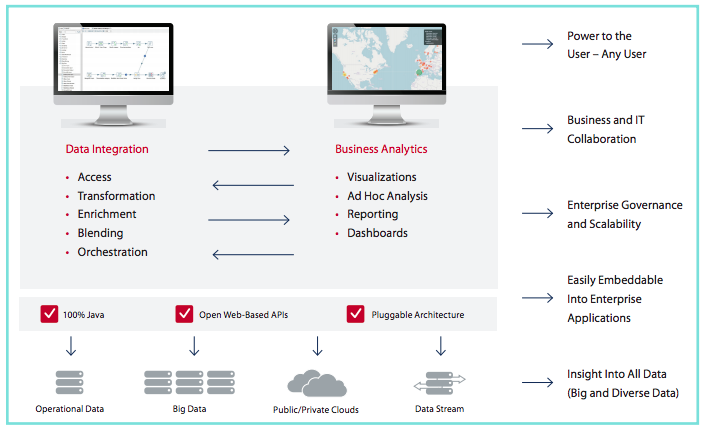
\includegraphics[width=0.6\textwidth]{./04-figuras/figura-15}
    \label{fig:ilustfig15}
\end{figure}
\vspace*{-0,9cm}
{\raggedright \fonte{Disponível em: <https://https://www.hitachivantara.com/en\_us/pdf/datasheet/pentaho-business-analytics-platform-datasheet.pdf>. Acesso em: 16 ago. 2020.}}\\

Os produtos Pentaho s\~{a}o abrangentes e usados para acessar, integrar, manipular, visualizar e analisar seus dados. Quer os dados sejam armazenados em um arquivo simples, banco de dados relacional, \textit{cluster Hadoop}, banco de dados NoSQL, banco de dados analítico, fluxos de mídia social, lojas operacionais ou na nuvem, os produtos Pentaho podem ajud\'{a}-lo a descobrir, analisar e visualizar dados para encontrar as respostas que você precisa, mesmo se você n\~{a}o tiver experiência em codifica\c{c}\~{a}o. 
Usu\'{a}rios avan\c{c}ados com experiência em programa\c{c}\~{a}o podem usar nossa ampla API\index{API}\footnote{API: Ë um conjunto de rotinas e padr\~{o}es de programa\c{c}\~{a}o para acesso a um aplicativo de software ou plataforma baseado na Web. A sigla API refere-se ao termo em inglês ``\textit{Application Programming Interface}'' que significa em tradu\c{c}\~{a}o para o português "Interface de Programa\c{c}\~{a}o de Aplicativos".} para personalizar relat\'orios, consultas e transforma\c{c}\~{o}es para estender a funcionalidade.

Os produtos Pentaho incluem componentes baseados na web e ferramentas de \textit{design}. Os componentes e ferramentas que você usa dependem do seu fluxo de trabalho e do que seu ambiente oferece suporte

Toda plataforma est\'{a} dividida em duas partes: Componentes baseados na web e as Ferramentas de \textit{Design}.

Os componentes baseados na web s\~{a}o:

\begin{itemize}
    \item Console de usu\'{a}rio: O \textit{Pentaho User Console} (PUC) \'{e} um ambiente de design para acessar \textit{Analyzer}, Relat\'orios Interativos e \textit{Dashboard Designer}. \textit{Pentaho User Console} tamb\'{e}m oferece recursos de administra\c{c}\~{a}o do sistema para configurar seu servidor Pentaho.
    
    \item Analisador: O \textit{Analyzer} ajuda a visualizar dados para tomar decis\~{o}es de neg\'ocios informadas. Você pode criar visualiza\c{c}\~{o}es geogr\'{a}ficas, gr\'{a}fico de dispers\~{a}o, grade de calor e múltiplos gr\'{a}ficos. Você tamb\'{e}m pode filtrar dados, adicionar parâmetros de consulta, configurar links de pesquisa detalhada, aplicar formata\c{c}\~{a}o condicional e gerar \textit{hiperlinks}. Em nosso trabalho iremos utilizar dois analisadores: o \textit{Saiku} e o \textit{JPivo}t.
    
    \item Relat\'orios Interativos: Relat\'orios interativos s\~{a}o uma interface de design usada para criar relat\'orios operacionais simples e sob demanda, sem depender de TI ou desenvolvedores de relat\'orios. Você pode adicionar rapidamente elementos ao seu relat\'orio e format\'{a}-los da maneira que desejar.
    
    \item \textit{Dashboard Designer}: O \textit{Dashboard Designer} \'{e} usado para escolher modelos de layout, temas e conteúdo para criar pain\'{e}is visualmente atraentes que ajudam os tomadores de decis\~{a}o a obter conhecimento crítico rapidamente. Você pode combinar uma ampla variedade de conteúdo, incluindo relat\'orios interativos, visualiza\c{c}\~{o}es do \textit{Analyzer} e conteúdo colaborativo.
    
    \item CTools: CTools \'{e} uma estrutura orientada pela comunidade para a cria\c{c}\~{a}o de pain\'{e}is usando tecnologias da web, como \textit{JavaScript}, CSS e HTML. Você pode criar facilmente pain\'{e}is dinâmicos para os usu\'{a}rios explorarem e entenderem grandes quantidades de dados usando uma variedade de gr\'{a}ficos, tabelas e outros componentes.
    
    \item Assistente de fonte de dados: O \textit{Data Source Wizard} ajuda a definir uma fonte de dados que cont\'{e}m suas informa\c{c}\~{o}es e o orienta na cria\c{c}\~{a}o de seus primeiros modelos relacionais ou multidimensionais para uso na cria\c{c}\~{a}o de relat\'orios e an\'{a}lises.
    
    \item Editor de modelo de fonte de dados: O Editor de modelo de fonte de dados ajuda a ajustar e refinar modelos de dados relacionais e multidimensionais. Você pode arrastar campos para seus locais apropriados, misturar e combinar campos de diferentes tabelas, adicionar campos a mais de uma categoria ou remover um campo.
\end{itemize}

As ferramentas de design da Pentaho s\~{a}o usadas para desenvolver e refinar como os valores dos dados s\~{a}o relatados, modelados, transformados e armazenados. Elas s\~{a}o:

\begin{itemize}
   \item Integra\c{c}\~{a}o de dados: \textit{Pentaho Data Integration} (PDI) fornece acesso a um motor de Extra\c{c}\~{a}o, Transforma\c{c}\~{a}o e Carregamento (ETL) que captura os dados certos, limpa os dados e armazena os dados usando um formato uniforme que \'{e} acessível e relevante para os usu\'{a}rios finais e tecnologias IoT\index{NewR}\footnote{IoT: \textit{Internet Of Tink} ou Internet das coisas \'{e} um conceito que se refere \`{a} interconex\~{a}o digital de objetos cotidianos com a internet, conex\~{a}o dos objetos mais do que das pessoas. Em outras palavras, a internet das coisas nada mais \'{e} que uma rede de objetos físicos capaz de reunir e de transmitir dados.}
   
   \item \textit{Report Designer}: O \textit{Report Designer} \'{e} usado para gerar relat\'orios detalhados e perfeitos em pixels, usando virtualmente qualquer fonte de dados. Ele permite que os profissionais de \textit{business intelligence} criem relat\'orios altamente detalhados e com qualidade de impress\~{a}o, com base em dados preparados de maneira adequada.

   \item Designer de agrega\c{c}\~{a}o: O \textit{Aggregation Designer} fornece uma interface simples que permite criar tabelas agregadas de níveis dentro das dimens\~{o}es que você especificar. Use esta ferramenta para melhorar o desempenho de seus cubos OLAP \textit{Pentaho Analysis} (Mondrian).

   \item Editor de Metadados: O Editor de Metadados simplifica a constru\c{c}\~{a}o de relat\'orios. Use o Editor de Metadados para construir domínios e modelos de metadados Pentaho. Um \textit{Pentaho Metadata Model} mapeia a estrutura física do seu banco de dados em um modelo de neg\'ocio l\'ogico.

    \item \textit{Schema Workbench}: \textit{Schema Workbench} permite editar e criar modelos multidimensionais (Mondrian). Você pode criar modelos Mondrian graficamente ou defini-los codificando manualmente os arquivos XML.
\end{itemize}

Nesta plataforma est\~{a}o disponíveis componentes para execu\c{c}\~{a}o de processos de ETL, que fazem carga de \textit{Data Warehouses}, cria\c{c}\~{a}o de relat\'orios pr\'{e}-formatados e ad hoc, cubos OLAP, pain\'{e}is de instrumentos (\textit{Dashboards}) e garimpagem de dados (\textit{Data Mining}). 

Todos esses recursos podem ser combinados e acionados sequencialmente para cria\c{c}\~{a}o de solu\c{c}\~{o}es mais sofisticadas. Al\'{e}m disso, a plataforma executa todas as solu\c{c}\~{o}es de BI como servi\c{c}os e, por isso, \'{e} possível prover acesso \`{a}s solu\c{c}\~{o}es para sistemas externos, via \textit{web services}, atrav\'{e}s de um mecanismo baseado em SOAP/WSDL/UDDI.

Por\'{e}m, n\~{a}o iremos neste trabalho nos deter em todos estes recurso, apenas o mínimo para uma solu\c{c}\~{a}o vi\'{a}vel para o servi\c{c}o do 181.

% DESENVOLVENDO A SOLU\c{c}\~{a}O

\section{Desenvolvimento da Solu\c{c}\~{a}o}

Com base nos conceitos do capitulo de Fundamenta\c{c}\~{a}o, e as t\'{e}cnicas de Kimball(2013), iremos aplicar estes conhecimentos na implementa\c{c}\~{a}o de um BI/DW, que ser\'{a} desenvolvido sobre um servidor local, usando todo o potencial e simplicidade da Plataforma Pentaho, desde o download do arquivo no formato ".XLS", com os dados de denúncias consultadas na aplica\c{c}\~{a}o web SISGOU, ao processamento ETL usando o PDI do Pentaho, e o OLAP usando o \textit{Saiku Analytics} e at\'{e} o \textit{dashboard} (painel) usando o CTOOLS e a cria\c{c}\~{a}o de um relat\'orio com o PRD.

% Banco de dados
\subsection{Criando nosso Banco de dados}

O nosso trabalho ir\'{a} precisar de um Banco de dados no SGBD PostgreSQL, que podemos criar via terminal do macOSX, por\'{e}m, usamos o aplicativo ``pgAdmin'' vers\~{a}o 4 que gerencia todos o banco de dados visualmente, economizando tempo de digita\c{c}\~{a}o, conforme figura abaixo.

\begin{figure}[H]
	\vspace*{0,2cm}
    \centering
    \caption{\textit{Script} do Banco de dados da solu\c{c}\~{a}o}
    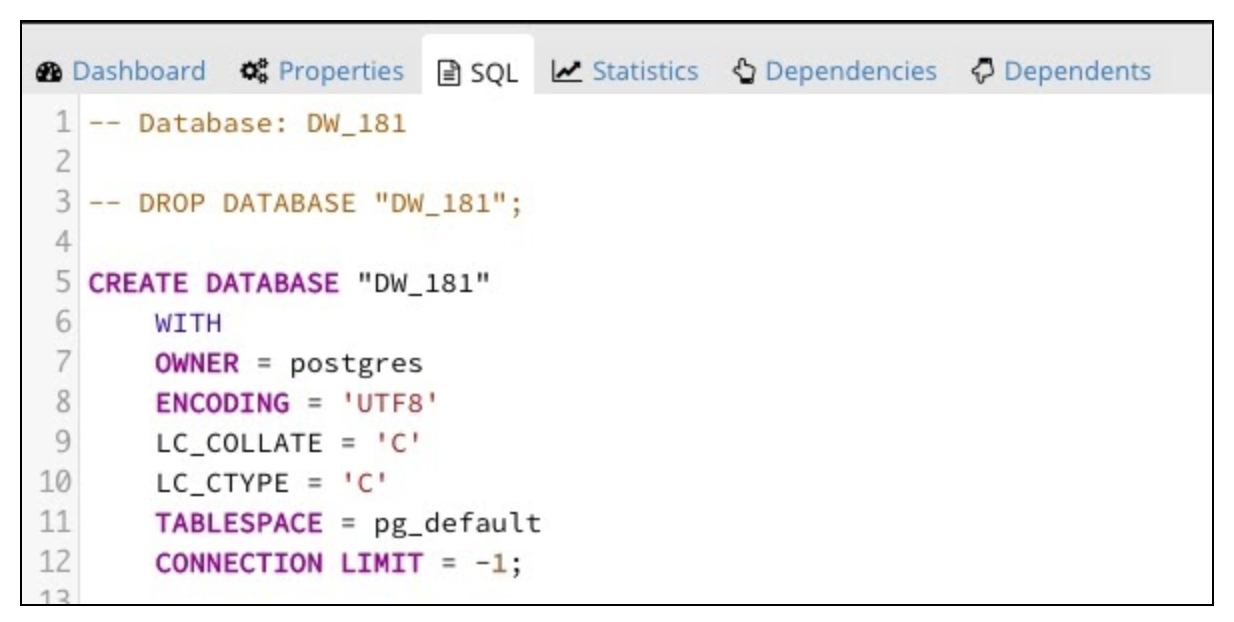
\includegraphics[width=0.6\textwidth]{./04-figuras/figura-16}
    \label{fig:ilustfig16}
\end{figure}
\vspace*{-0,9cm}
{\raggedright \fonte{Autor desta monografia, 2020.}} \\

Acessando o ``pdAmin'', e digitando esse comando da figura acima e basta apenas executar o mesmo na ferramenta que o Banco de dados ser\'{a} criando. Iniciando assim o primeiro passado para criarmos nossa ETL.

\subsection{Criando o processo de ETL}

Ap\'os termos dado o primeiro passo, teremos como base do processo de Extra\c{c}\~{a}o o arquivo no formato do \textit{Microsoft Excel} denominado ``181.xls'', lembrando que o mesmo foi exportado ``do Aplicativo Web SISGOU'' na op\c{c}\~{a}o de consulta. 
Ele ter\'{a} o mesmo formado da figura abaixo, como suas linhas e colunas totalmente sem normatiza\c{c}\~{a}o aparente e sem nenhum tratamento nos dados.

% FALTA A figura

\begin{figure}[H]
	\vspace*{0,2cm}
    \centering
    \caption{Arquivo extraído da consulta do Disque denúncia do  SISGOU}
    \includegraphics[width=0.6\textwidth]{./04-figuras/figura-arquivo-xls}
    \label{fig:ilustfigxls}
\end{figure}
\vspace*{-0,9cm}
{\raggedright \fonte{Autor desta monografia, 2020.}} \\

Para criarmos nosso processo de ETL no arquivo acima, precisamos usar o \textit{Pentaho Data Integration}, para isso precisamos instalar o mesmo junto com toda Plataforma Pentaho. E ap\'os instalado,  clicaremos com o mouse no ícone do \textint{Data Integration}, a tela de boas vindas do PDI aparece, de acordo com a figura abaixo e depois surge a interface da aplica\c{c}\~{a}o que ser\'{a} usada para a configura\c{c}\~{a}o dos processo de ETL, que transformar\~{a}o os dados em \textit{Microsoft Excel} com dados formatado por um SGBD relacional.

\begin{figure}[H]
	\vspace*{0,2cm}
    \centering
    \caption{tela de Boas Vinda e a Interface do PDI (\textit{Pentaho Data Integration}).}
    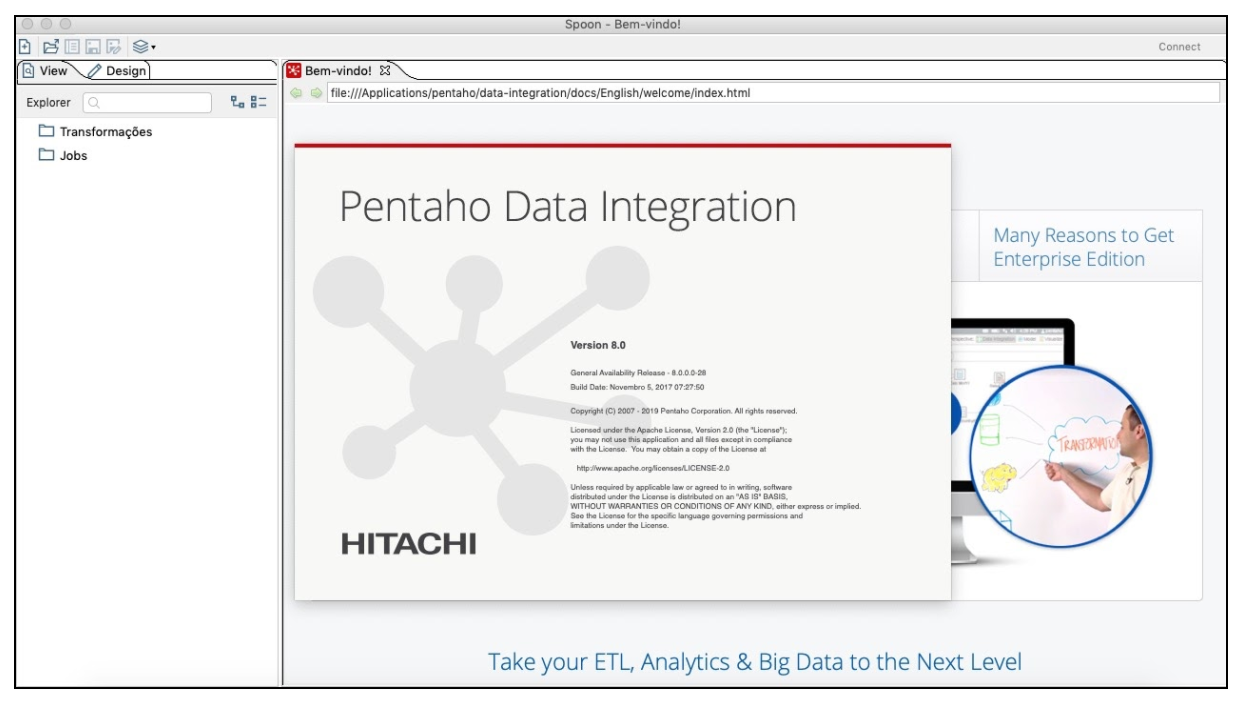
\includegraphics[width=0.6\textwidth]{./04-figuras/figura-pentaho-pdi}
    \label{fig:ilustfigpentaho-pdi}
\end{figure}
\vspace*{-0,9cm}
{\raggedright \fonte{Autor desta monografia, 2020.}} \\

O \textit{Pentaho Data Integration}, fornece os recursos \textit{Extract, Transform e Load} (ETL) que facilitam o processo de captura, limpeza e armazenamento de dados usando um formato uniforme e consistente que \'{e} acessível e relevante para os usu\'{a}rios finais e tecnologias IoT.

O PDI \'{e} formado por duas categorias de artefatos, \textit{Jobs} e Transforma\c{c}\~{o}es, e estes artefatos s\~{a}o construídos por meio de sua interface gr\'{a}fica, o \textit{Spoon}. 

O \textit{Spoon} \'{e} a interface gr\'{a}fica do \textit{Pentaho Data Integration} que facilita na concep\c{c}\~{a}o de rotinas e l\'ogica ETL. Abaixo na figura apresentamos a interface do PDI.

\begin{figure}[H]
	\vspace*{0,2cm}
    \centering
    \caption{Spoon do PDI (\textit{Pentaho Data Integration}).}
    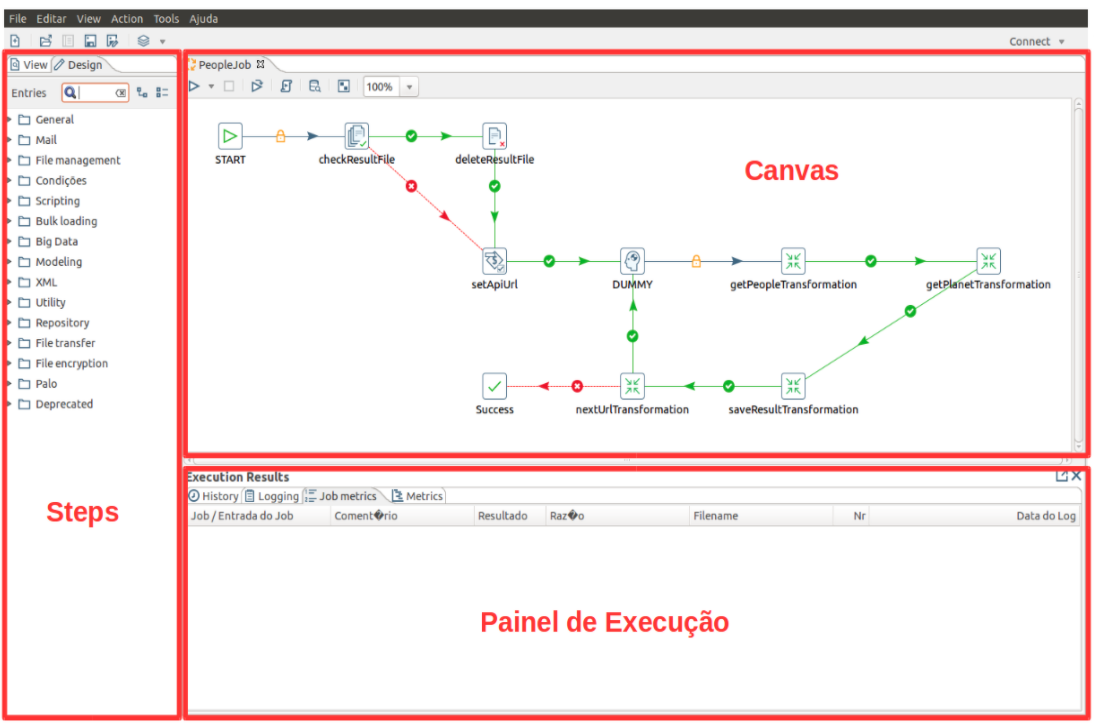
\includegraphics[width=0.6\textwidth]{./04-figuras/figura-pentaho-pdi-spoon}
    \label{fig:ilustfigpentaho-pdi-spoon}
\end{figure}
\vspace*{-0,9cm}
{\raggedright \fonte{Autor desta monografia, 2020.}} \\

Que ser\~{a}o nomeadas no banco de dados ``DW\_181'' como: dim\_bairro, dim\_cidade, dim\_origem, dim\_tipo-denncia, dim\_data, dim\_hora e o fato\_denuncia.

Quando todas as transforma\c{c}\~{o}es das dimens\~{o}es e do fato forem desenvolvidas iremos uní-las em um processo denominado \textit{Job}, que agregar\'{a} todas as transforma\c{c}\~{o}es para uma execu\c{c}\~{a}o única de toda ETL.

O primeiro passo \'{e} criar a conex\~{a}o usando o componente \textit{Database Connection}, em nosso trabalho usaremos o nome ``CNN\_DW\_181'' para a conex\~{a}o com o banco de dados local ``DW\_181'', na porta de número: ``5432'', usu\'{a}rio: ``postgres'', conforme figura abaixo.

\begin{figure}[H]
	\vspace*{0,2cm}
    \centering
    \caption{\textit{Database Connection - ``CNN\_DW\_181''}}
    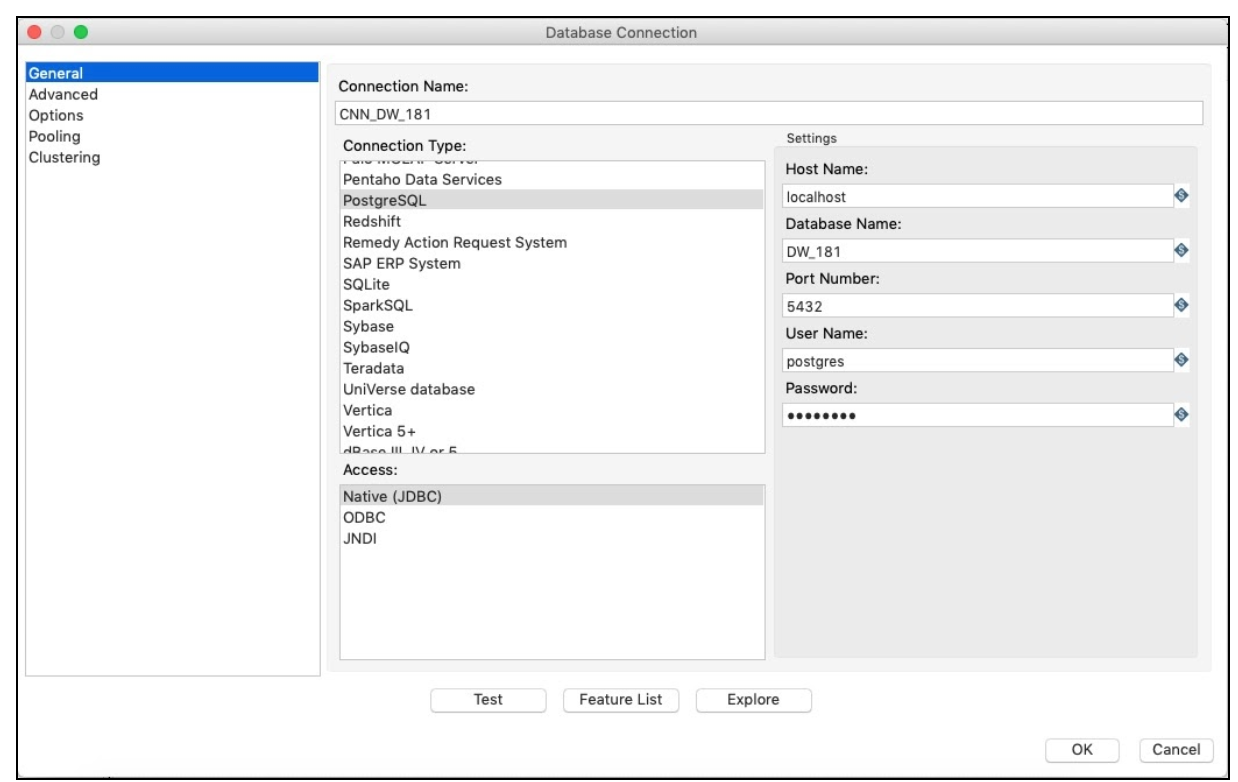
\includegraphics[width=0.6\textwidth]{./04-figuras/figura-pentaho-database-connection}
    \label{fig:ilustfigpentaho-database-connection}
\end{figure}
\vspace*{-0,9cm}
{\raggedright \fonte{Autor desta monografia, 2020.}} \\

% TRANSFORMA\c{c}\~{o}ES
\subsubsection{Criando as transforma\c{c}\~{o}es no PDI}

Ap\'os a termos criado no t\'opico anterior a conex\~{a}o ``CNN\_DW\_181'', iniciaremos a desenvolvimento das transforma\c{c}\~{o}es. Para isso se faz necess\'{a}rio o uso de alguns \textint{steps}. que iniciam do do acesso aos dados no arquivo com os dados a serem transformado at\'{e} a cria\c{c}\~{a}o e carga da dimens\~{a}o que far\~{a}o parte do modelo Dimensional Estrela j\'{a} definido neste trabalho.

Para criarmos as transforma\c{c}\~{o}es que ao final sejam geradas \`{a}s dimens\~{o}es, precisamos usar a aba \textit{Design} e os componentes nela presentes.

Para melhorar o entendimento padronizamos um nomenclatura para os arquivos das transforma\c{c}\~{o}es, formato ``.ktr'', e do \textit{Job}\index{job}\footnote{\textit{Job}: \'{e} o processo que une todas \`{a}s transforma\c{c}\~{o}es para uma execu\c{c}\~{a}o de todas dentro do PDI}, formato ``.kjb'', para ajudar no desenvolvimento do DW/BI. Para transforma\c{c}\~{o}es de dimens\~{o}es: ``dim\_nome da dimens\~{a}o.ktr'' e para o fato: ``fato\_nome do fato.ktr
''.

Na constru\c{c}\~{a}o das nossas transforma\c{c}\~{o}es e nesta fase de ETL como um todo utilizaremos o componente de step: \textit{Microsoft Excel Input}, figura abaixo, que est\'{a} localizado na barra lateral de Design do \textit{Spoon}, na categoria \textit{input}. Este componente em especial ser\'{a} o padr\~{a}o para o acesso aos dados da planilha em no formato do \textit{Microsoft Excel}, e nome ``181.xls'' em todas as transforma\c{c}\~{o}es.

O \textit{step Microsoft Excel Input} tem como principais fun\c{c}\~{o}es dar acesso ao dados e fazer ajustes nos nomes, tipos e tamanhos das colunas.

\begin{figure}[H]
	\vspace*{0,2cm}
    \centering
    \caption{Barra lateral do PDI e o Componente \textit{step Microsoft Excel Input}}
    \includegraphics[width=0.6\textwidth]{./04-figuras/figura-pentaho-pdi-step-mei}
    \label{fig:ilustfigpentahopdistepmei}
\end{figure}
\vspace*{-0,9cm}
{\raggedright \fonte{Autor desta monografia, 2020.}} \\

Quando acessamos o \textit{step Microsoft Excel Input} temos acesso a tela conforme da figura abaixo, nela temos as abas \textit{Files, Sheets, Content, Error Handing, Fields e Additional output fields}. Por\'{e}m, vamos apenas nos focar na aba \textit{Fields} que cont\'{e}m os campos providos da fonte de dados. 

Nela podemos fazer os ajustes necess\'{a}rios para que a transforma\c{c}\~{a}o ao longo dos \textit{steps Select values, Sort rows, Unique rows, Value Mapper, Add sequence, Table output} recebam os dados n\~{a}o transformados que ser\~{a}o ao longo dos \textit{steps} ajustados para que ao final tenhamos a dimens\~{a}o pretendida com os dados padronizados .

\begin{figure}[H]
	\vspace*{0,2cm}
    \centering
    \caption{Componente \textit{step Microsoft Excel Input}}
    \includegraphics[width=0.6\textwidth]{./04-figuras/figura-pentaho-pdi-step-meis}
    \label{fig:ilustfigpentahopdistepmeis}
\end{figure}
\vspace*{-0,9cm}
{\raggedright \fonte{Autor desta monografia, 2020.}} \\

% Transforma\c{c}\~{o}es

% dim\_bairros.ktr
\subsubsection{Criando a transforma\c{c}\~{a}o ``dim\_bairro.ktr''}

Os componentes que far\~{a}o parte da transforma\c{c}\~{a}o ``dim\_bairro.ktr'', ser\~{a}o: \textit{Microsoft Excel Input, Select values, Sort rows, Unique rows, Value Mapper, Add sequence} e finalmente \textit{Table Table output} conforme figura abaixo.

\begin{figure}[H]
	\vspace*{0,2cm}
    \centering
    \caption{Componente \textit{step Microsoft Excel Input.}}
    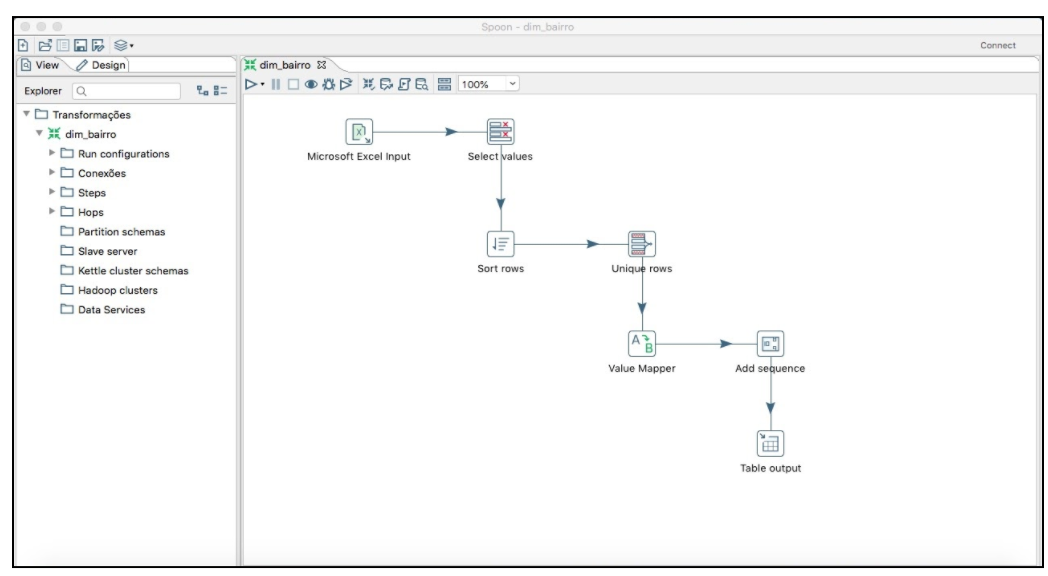
\includegraphics[width=0.6\textwidth]{./04-figuras/figura-dim-bairro}
    \label{fig:ilustfigdimbairro}
\end{figure}
\vspace*{-0,9cm}
{\raggedright \fonte{Autor desta monografia, 2020.}} \\

Primeiramente iremos configurar o \textit{step Select Value} (Selecione o Valor), e na aba \textit{Select & Alter}, na op\c{c}\~{a}o \textit{Fields, Rename to}, iremos modificar o nome Bairro para ``ds\_bairro'', nesse componente ser\'{a} apenas essa a altera\c{c}\~{a}o, conforme figura do quadro tela do \textit{step Select Value}.

Ap\'os  componente \textit{Select Value}, iremos configurar o \textit{step Sort rows} (Organizar a linha), na op\c{c}\~{a}o \textit{Fields}, \textit{Ascending} como ``S'', para que os dados fiquem organizado de forma ascendente, figura do quadro tela do \textit{step Sort rows}.

O pr\'oximo componente \'{e} \textit{Unique rows} que tem a característica de selecionar apenas os valores únicos das linhas, ou seja, evitar a duplica\c{c}\~{a}o, nesse componente h\'{a} apenas a necessidade de configurar o nome do campo ou \textit{Fieldname}, conforme a figura da tela do \textit{step Unique rows}.

O componente \textit{Value Mapper}, em síntese tem como fun\c{c}\~{a}o trocar os valores vindos da linha da fonte de dados que ser\~{a}o comparados no \textit{Source Value}, e ap\'os encontrar o mesmo ela ser\'{a} trocado pelo informado em \textit{Target value}, conforme a figura da tela do \textit{step Value Mapper}.

Ap\'os transformarmos os dados brutos da linha Bairro da fonte de dado em Ms \textit{Microsoft Excel}, iremos criar um campo sequencial, para isso usaremos o componente \textit{Add sequence}, a única altera\c{c}\~{a}o ser\'{a} no op\c{c}\~{a}o Nome do valor, que foi mudado para ``id\_bairro'', conforme figura da tela do \textit{Add sequence}.

Finalizando a transforma\c{c}\~{a}o ``dim\_bairro.ktr'', usaremos o componente \textit{Table output} nele iremos alterar as op\c{c}\~{o}es \textit{Connection, Target schema, Target table, truncate table}, e na aba \textit{Database fields}, incluiremos os Campos ou colunas da tabela ``dim\_bairro'' que ser\'{a} criada ap\'os finalizar essa etapa de configura\c{c}\~{a}o dos componentes da transforma\c{c}\~{a}o, conforme \`{a} figura da tela do \textit{step Table output}.

\begin{figure}[H]
	\vspace*{0,2cm}
    \centering
    \caption{Configurando os \textit{steps} da Transforma\c{c}\~{a}o ``dim\_bairros.ktr''(passo-a-passo).}
    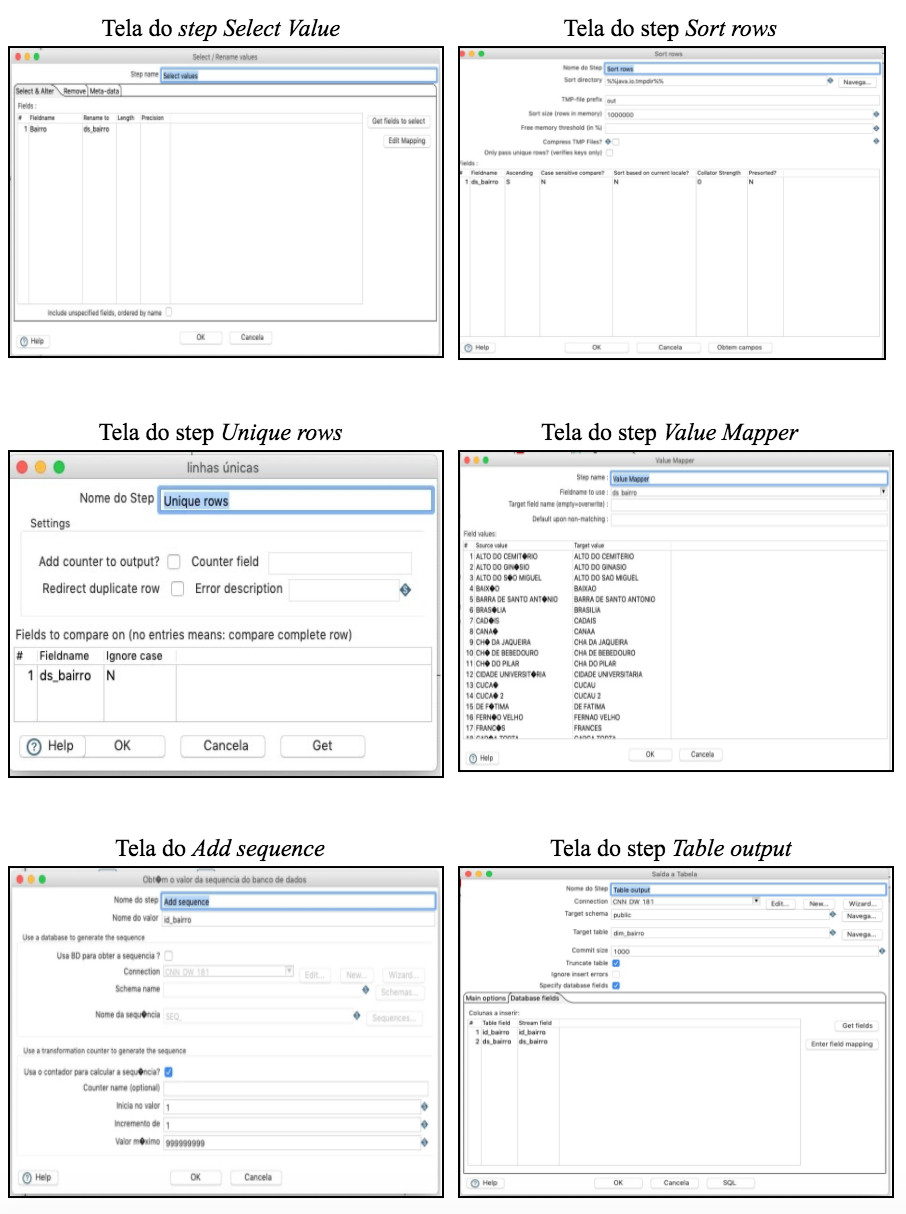
\includegraphics[width=0.6\textwidth]{./04-figuras/figura-passos-dim-bairros}
    \label{fig:ilustfigpassasdimbairros}
\end{figure}
\vspace*{-0,9cm}
{\raggedright \fonte{Autor desta monografia, 2020.}} \\

Ap\'os ter ajustado a configura\c{c}\~{a}o do \textit{step Table output}, selecionaremos o bot\~{a}o SQL, e aparecer\'{a} a tela da figura abaixo, tela \textit{Simple SQL editor}. Na tela do \textit{Simple SQL editor} , selecionando o bot\~{a}o \textit{Execute}, e surgir\'{a} a tela \textit{Results of the SQL statements}, conforme figura abaixo, abaixo. E finalmente criamos o tabela ``dim\_bairro'', dentro do banco de dados 
``DW\_181''.

\begin{figure}[H]
	\vspace*{0,2cm}
    \centering
    \caption{Criando a tabela ``dim\_bairro'' no banco de dados usando o \textit{step Table output}}
    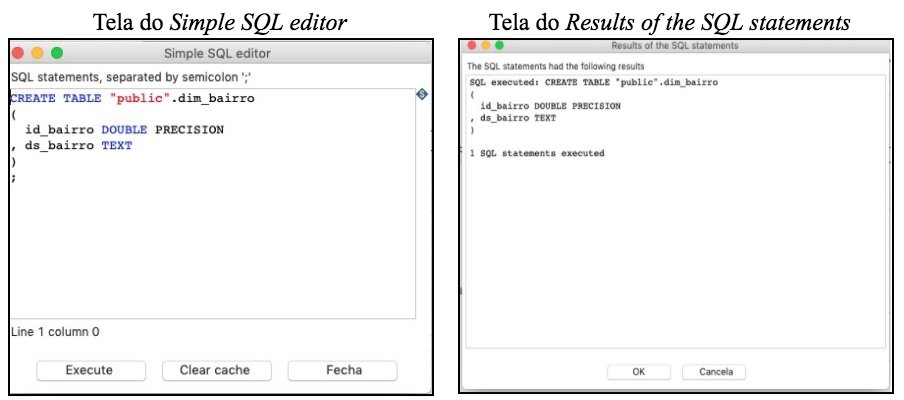
\includegraphics[width=0.6\textwidth]{./04-figuras/figura-tb-dim-bairro}
    \label{fig:ilustfigtbdimbairros}
\end{figure}
\vspace*{-0,9cm}
{\raggedright \fonte{Autor desta monografia, 2020.}} \\

% dim\_cidade.ktr
\subsubsection{Criando a transforma\c{c}\~{a}o ``dim\_cidade.ktr''}

Os componentes que far\~{a}o parte da transforma\c{c}\~{a}o ``dim\_cidade.ktr'', ser\~{a}o: \textit{Microsoft Excel Input, Select values, Sort rows, Unique rows, Value Mapper, Add sequence} e finalmente \textit{Table Table output} conforme figura sabaixo. 

\begin{figure}[H]
	\vspace*{0,2cm}
    \centering
    \caption{Transforma\c{c}\~{a}o ``dim\_cidade.ktr''}
    \includegraphics[width=0.6\textwidth]{./04-figuras/figura-transf-dim-cidade}
    \label{fig:ilustfigtransfdimcidade}
\end{figure}
\vspace*{-0,9cm}
{\raggedright \fonte{Autor desta monografia, 2020.}} \\

Primeiramente iremos configurar o \textit{step Select Value} (Selecione o Valor), e na aba \textit{Select & Alter}, na op\c{c}\~{a}o \textit{Fields, Rename to}, teremos que modificar o nome Bairro para ``ds\-bairro'', nesse componente ser\'{a} apenas essa a altera\c{c}\~{a}o, conforme figura do quadro tela do \textit{step Select Value}.

Ap\'os  componente \textit{Select Value}, iremos configurar o \textit{step Sort rows} (Organizar a linha), na op\c{c}\~{a}o \textit{Fields, Ascending} como ``S'', para que os dados fiquem organizado de forma ascendente, figura do quadro tela do \textit{step Sort rows}.

O pr\'oximo componente \'{e} \textit{Unique rows} que tem a característica de selecionar apenas os valores únicos das linhas, ou seja, evitar a duplica\c{c}\~{a}o, nesse componente h\'{a} apenas a necessidade de configurar o nome do campo ou \textit{Fieldname}, conforme a figura da tela do \textit{step Unique rows}.

O componente \textit{Value Mapper}, em síntese tem como fun\c{c}\~{a}o trocar os valores vindos da linha da fonte de dados que ser\~{a}o comparados no \textit{Source Value}, e ap\'os encontrar o mesmo ela ser\'{a} trocado pelo informado em \textit{Target value}, conforme a figura do quadro tela do \textit{step Value Mapper}.

Ap\'os transformarmos os dados brutos da linha ``Cidade'' da fonte de dado em \textit{Microsoft Excel}, iremos criar um campo sequencial, para isso usaremos o componente \textit{Add sequence}, a única altera\c{c}\~{a}o ser\'{a} no op\c{c}\~{a}o Nome do valor, que foi mudado para ``id\_cidade'', conforme figura da tela do \textit{Add sequence}.

Finalizando a transforma\c{c}\~{a}o ``dim\_cidade.ktr'', usaremos o componente Table output nele iremos alterar as op\c{c}\~{o}es \textit{Connection, Target schema, Target table, truncate table}, e na aba \textit{Database fields}, incluiremos os Campos ou colunas da tabela ``dim\_cidade'' que ser\'{a} criada ap\'os finalizar essa etapa de configura\c{c}\~{a}o dos componentes da transforma\c{c}\~{a}o, conforme a figura da tela do \textit{step Table output}.

\begin{figure}[H]
	\vspace*{0,2cm}
    \centering
    \caption{Configurando os \textit{steps} da Transforma\c{c}\~{a}o ``dim\_cidade.ktr'' (passo-a-passo)}
    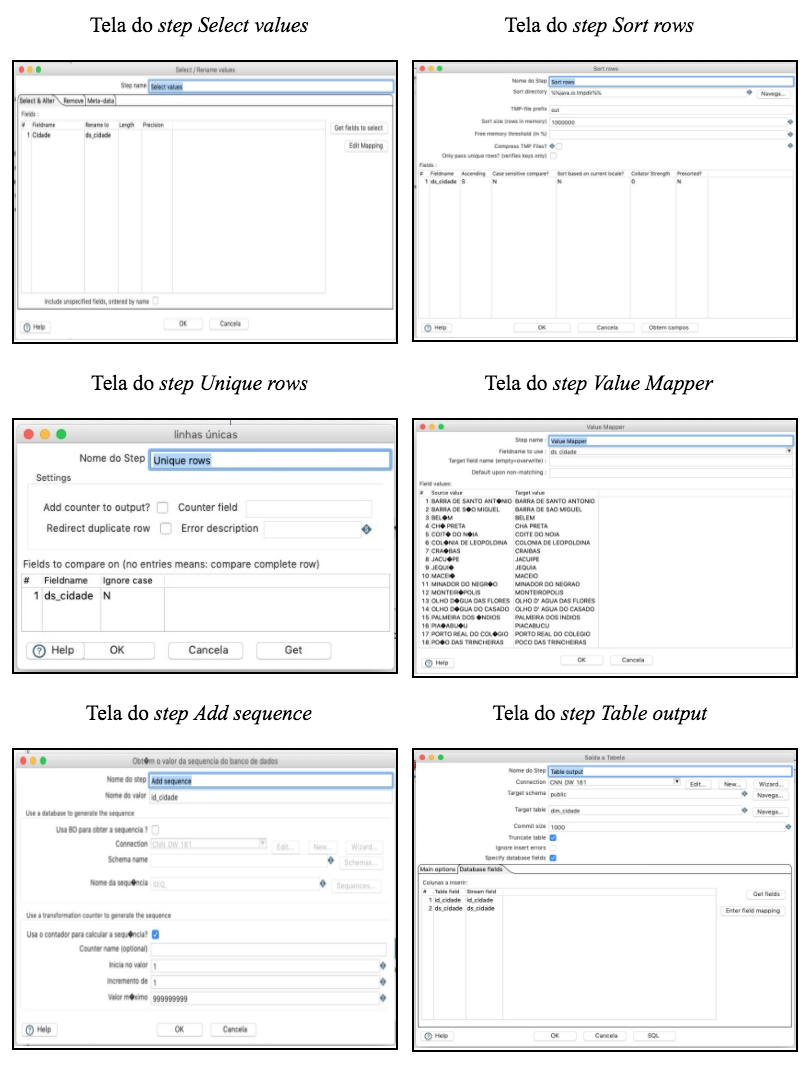
\includegraphics[width=0.6\textwidth]{./04-figuras/figura-step-dim-cidade}
    \label{fig:ilustfigstepdimcidade}
\end{figure}
\vspace*{-0,9cm}
{\raggedright \fonte{Autor desta monografia, 2020.}} \\

\begin{figure}[H]
	\vspace*{0,2cm}
    \centering
    \caption{Criando a tabela ``dim\_cidade'' no banco de dados usando o \textit{step Table output}}
    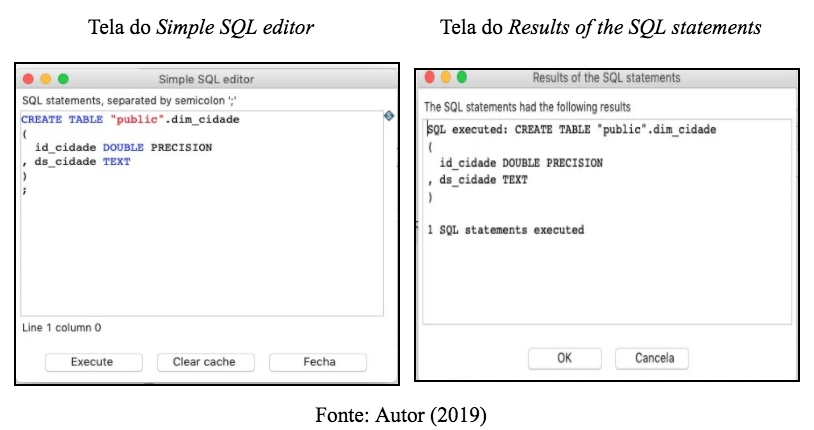
\includegraphics[width=0.6\textwidth]{./04-figuras/figura-tb-dim-cidade}
    \label{fig:ilustfigtbdimcidade}
\end{figure}
\vspace*{-0,9cm}
{\raggedright \fonte{Autor desta monografia, 2020.}} \\

Ao final dos processos quando executamos a transforma\c{c}\~{a}o, conforme figura abaixo, na parte posterior da tela do PDI, em ``Execution Results''. aparecer\'{a} na aba ``Preview data'', os dados padronizados dos campos: ``ds\_cidade'' e ``id\_cidade''. O pr\'oximo passo ser\'{a} percorrer a grade com os resultado e perceber se o processo de transforma\c{c}\~{a}o e carga sai conforme planejado. 

\begin{figure}[H]
	\vspace*{0,2cm}
    \centering
    \caption{Executando a transforma\c{c}\~{a}o ``dim\_cidade.ktr'' (passo-a-passo)}
    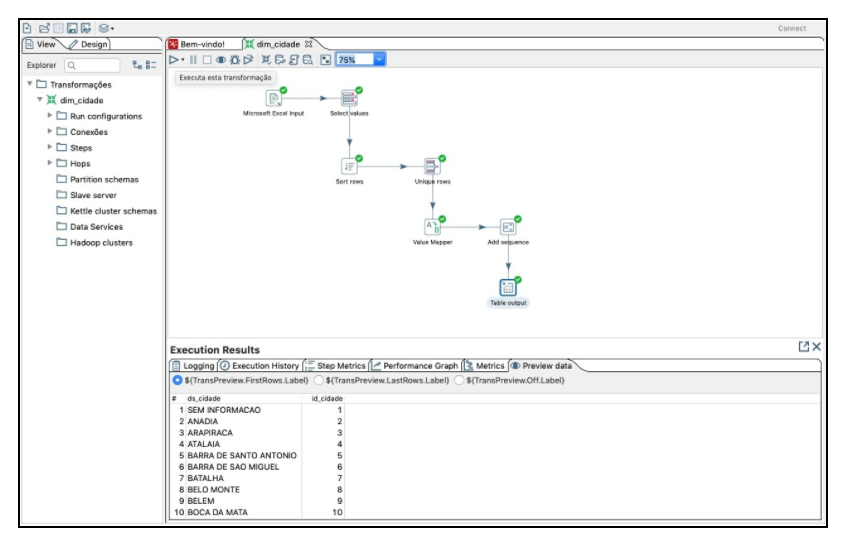
\includegraphics[width=0.6\textwidth]{./04-figuras/figura-exec-dim-cidade}
    \label{fig:ilustfigexecdimcidade}
\end{figure}
\vspace*{-0,9cm}
{\raggedright \fonte{Autor desta monografia, 2020.}} \\

Para termos a certeza de que a tabela ``dim\_cidade'', obteve a ETL correta, precisamos abrir a tabela ``dim\_cidade'' no aplicativo ``pgAdmin 4'', que \'{e} instalado junto ao PostgreSQL, conforme figura abaixo, nela podemos analisar os dados processados pela transforma\c{c}\~{a}o criada no PDI: ``dim\_cidade.ktr''.

\begin{figure}[H]
	\vspace*{0,2cm}
    \centering
    \caption{Resultado da transforma\c{c}\~{a}o e carga no Banco de Dados ``DW\_181'' na tabela ``dim\_cidade''}
    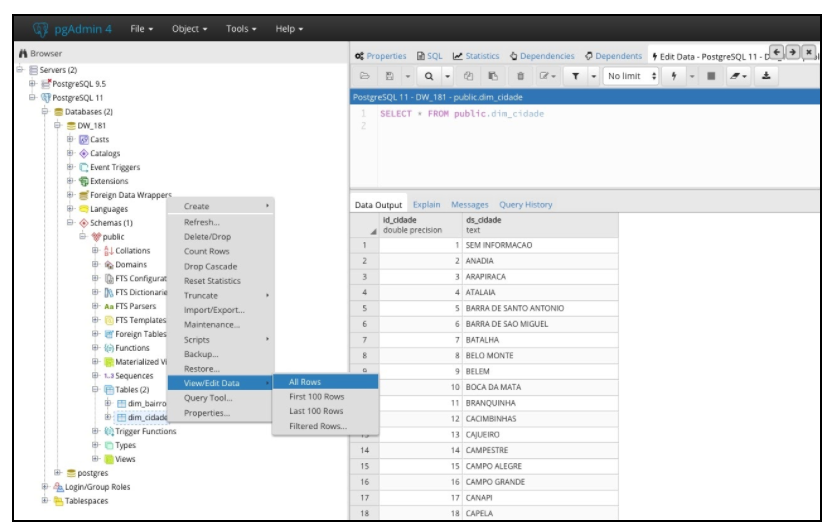
\includegraphics[width=0.6\textwidth]{./04-figuras/figura-result-dim-cidade}
    \label{fig:ilustfigresultdimcidade}
\end{figure}
\vspace*{-0,9cm}
{\raggedright \fonte{Autor desta monografia, 2020.}} \\

% dim\_tipo\_denuncia.ktr
\subsubsection{Criando a transforma\c{c}\~{a}o ``dim\_tipo-denuncia.ktr''}

Os componentes que far\~{a}o parte da transforma\c{c}\~{a}o ``dim\_tipo\_denuncia.ktr'', ser\~{a}o: \textit{Microsoft Excel Input, Select values, Sort rows, Unique rows, Value Mapper, Add sequence} e finalmente \textit{Table Table output} conforme figura abaixo. 

\begin{figure}[H]
	\vspace*{0,2cm}
    \centering
    \caption{Transforma\c{c}\~{a}o ``dim\_tipo\_denuncia.ktr'' do BI do 181.}
    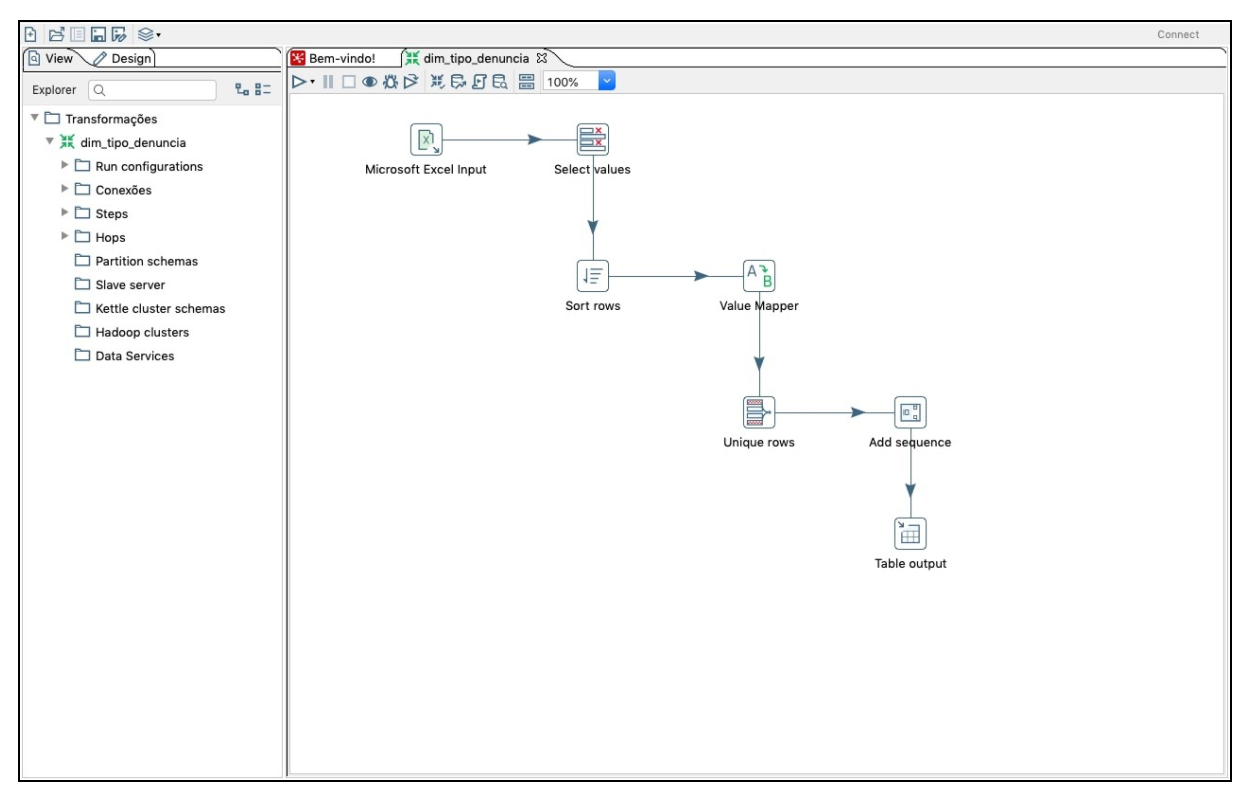
\includegraphics[width=0.6\textwidth]{./04-figuras/figura-dim-tipo-denuncia}
    \label{fig:ilustfigrdimtipodenuncia}
\end{figure}
\vspace*{-0,9cm}
{\raggedright \fonte{Autor desta monografia, 2020.}} \\

Primeiramente iremos configurar o \textit{step Select Value} (Selecione o Valor), e na aba \textit{Select & Alter}, na op\c{c}\~{a}o \textit{Fields, Rename to}, iremos modificar o nome Bairro para ``ds\_tipo\_denuncia'', nesse componente ser\'{a} apenas essa a altera\c{c}\~{a}o, conforme figura da tela da \textit{step Select Value}.

Ap\'os  componente \textit{Select Value}, iremos configurar o \textit{step Sort rows} (Organizar a linha), na op\c{c}\~{a}o \textit{Fields, Ascending} como ``S'', para que os dados fiquem organizado de forma ascendente, figura da tela do \textit{step Sort rows}.

O pr\'oximo componente \'{e} \textit{Unique rows} que tem a característica de selecionar apenas os valores únicos das linhas, ou seja, evitar a duplica\c{c}\~{a}o, nesse componente h\'{a} apenas a necessidade de configurar o nome do campo ou \textit{Fieldname}, conforme a figura da tela do \textit{step Unique rows}.

O componente \textit{Value Mapper}, em síntese tem como fun\c{c}\~{a}o trocar os valores vindos da linha da fonte de dados que ser\~{a}o comparados no \textit{Source Value}, e ap\'os encontrar o mesmo ela ser\'{a} trocado pelo informado em \textit{Target value}, conforme a figura da tela do \textit{step Value Mapper}.

Ap\'os transformarmos os dados brutos da linha ``tipo\ denuncia'' da fonte de dado em \textit{Microsoft Excel}, iremos criar um campo sequencial, para isso usaremos o componente \textit{Add sequence}, a única altera\c{c}\~{a}o ser\'{a} no op\c{c}\~{a}o Nome do valor, que foi mudado para ``id\_tipo\_denuncia'', conforme figura da tela do \textit{Add sequence}.

Finalizando a transforma\c{c}\~{a}o ``dim\_tipo\_denuncia.ktr'', usaremos o componente \textit{Table output} nele iremos alterar as op\c{c}\~{o}es \textit{Connection, Target schema, Target table, truncate table}, e na aba \textit{Database fields}, incluiremos os Campos ou colunas da tabela ``dim\_tipo\_denuncia'' que ser\'{a} criada ap\'os finalizar essa etapa de configura\c{c}\~{a}o dos componentes da transforma\c{c}\~{a}o, conforme a figura da tela do \textit{step Table output}.

\begin{figure}[H]
	\vspace*{0,2cm}
    \centering
    \caption{Configurando os \testit{steps} da Transforma\c{c}\~{a}o ``dim\_tipo\_denuncia.ktr'' (passo-a-passo)}
    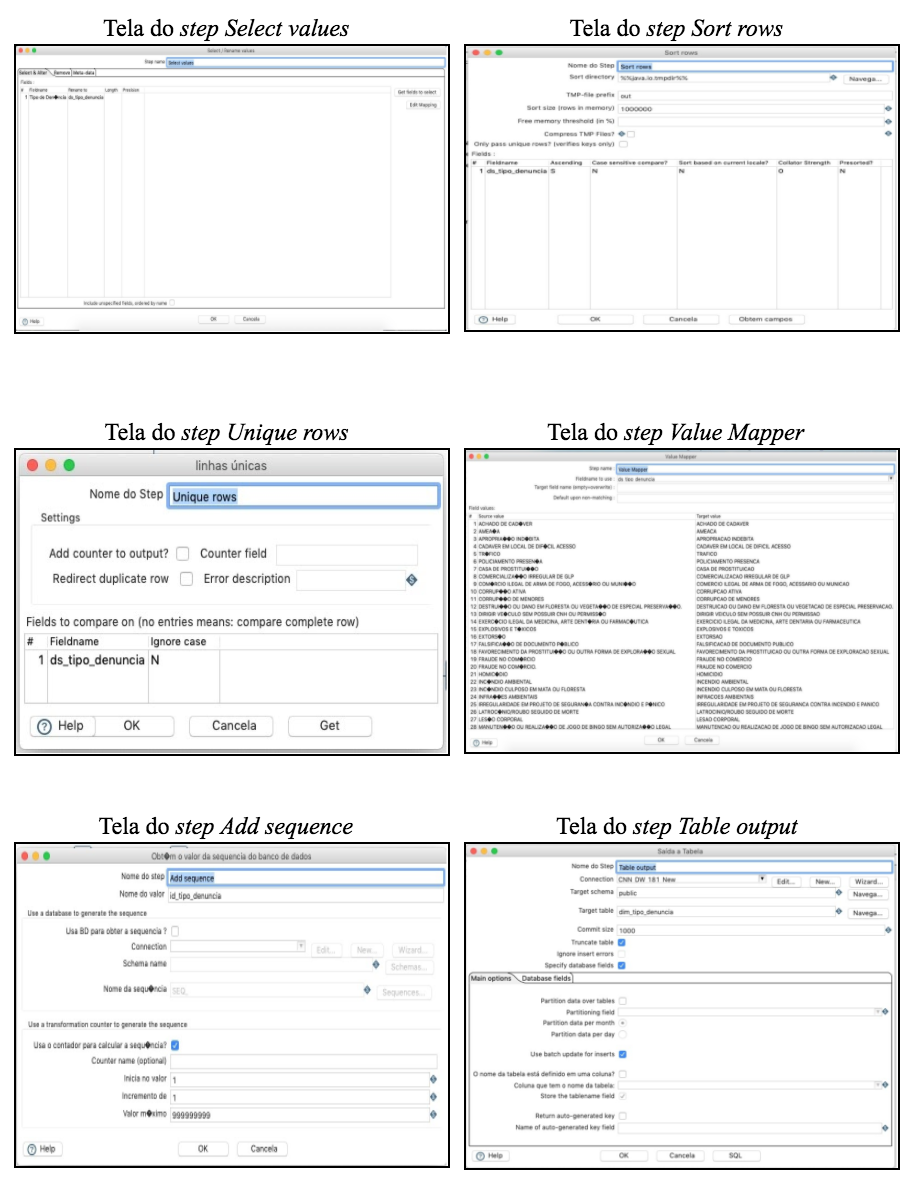
\includegraphics[width=0.6\textwidth]{./04-figuras/figura-dim-tipo-denuncia-passo-a-passo}
    \label{fig:ilustfigrdimtipodenunciapassoapasso}
\end{figure}
\vspace*{-0,9cm}
{\raggedright \fonte{Autor desta monografia, 2020.}} \\

\begin{figure}[H]
	\vspace*{0,2cm}
    \centering
    \caption{Criando a tabela ``dim\_tipo\_denuncia'' no banco de dados usando o \testit{step Table output}}
    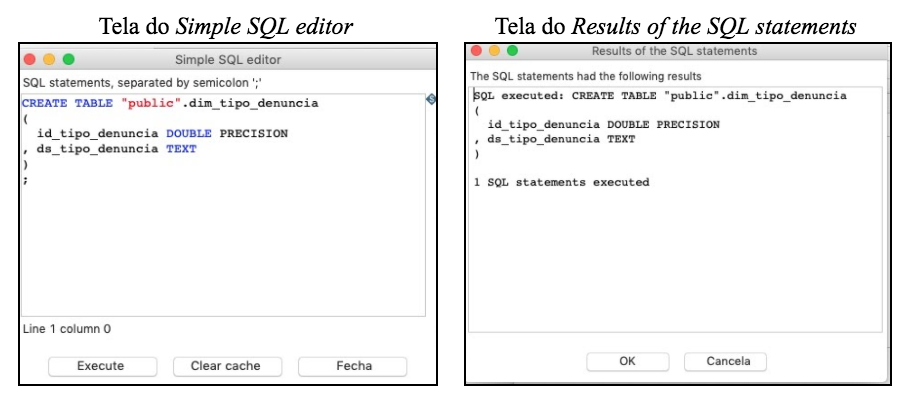
\includegraphics[width=0.6\textwidth]{./04-figuras/figura-tb-dim-tipo-denuncia}
    \label{fig:ilustfigtbdimtipodenuncia}
\end{figure}
\vspace*{-0,9cm}
{\raggedright \fonte{Autor desta monografia, 2020.}} \\

Ao final dos processos quando executamos a transforma\c{c}\~{a}o, conforme figura 48, na parte posterior da tela do PDI, em \textit{Execution Results}. aparecer\'{a} na aba \textit{Preview data}, os dados padronizados dos campos: ``ds\_tipo\_denuncia'' e ``id\_tipo\_denuncia''. O pr\'oximo passo ser\'{a} percorrer a grade com os resultado e perceber se o processo de transforma\c{c}\~{a}o e carga sai conforme planejado. 

\begin{figure}[H]
	\vspace*{0,2cm}
    \centering
    \caption{Executando a transforma\c{c}\~{a}o ``dim\_tipo\_denuncia.ktr''}
    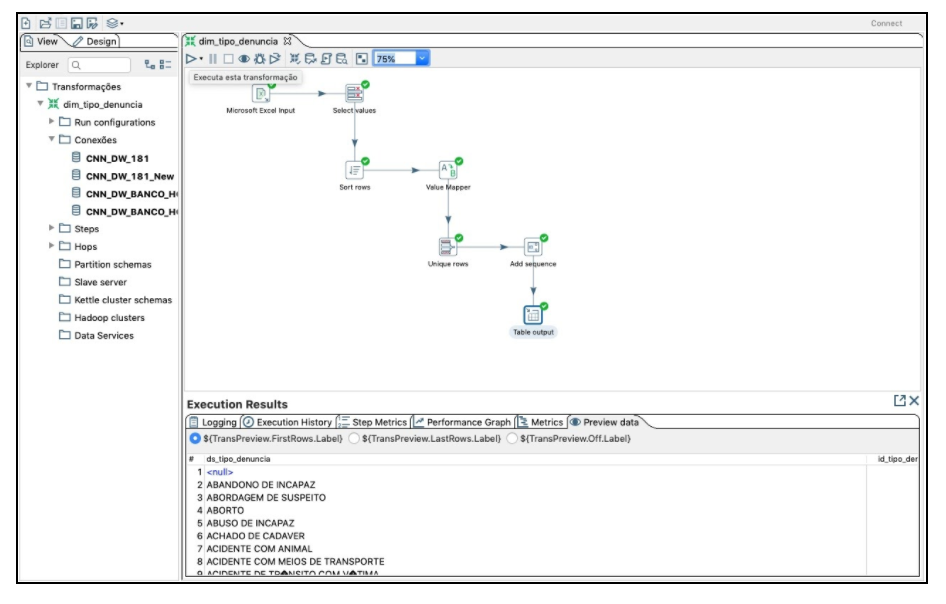
\includegraphics[width=0.6\textwidth]{./04-figuras/figura-trans-tipo-denuncia}
    \label{fig:ilustfigtranstipodenuncia}
\end{figure}
\vspace*{-0,9cm}
{\raggedright \fonte{Autor desta monografia, 2020.}} \\

Para se ter certeza de que a tabela ``dim\_tipo\_denuncia'', obteve a ETL correta, precisamos abrir a tabela ``dim\_tipo\_denuncia'' no aplicativo pgAdmin vers\~{a}o 4, que \'{e} instalado junto ao PostgreSQL, conforme figura 49, nela podemos analisar os dados processados pela transforma\c{c}\~{a}o criada no PDI: ``dim\_tipo\_denuncia.ktr''.

\begin{figure}[H]
	\vspace*{0,2cm}
    \centering
    \caption{Resultado da transforma\c{c}\~{a}o e carga no Banco de Dados ``DW\_181'' na tabela ``dim\_tipo\_denuncia''}
    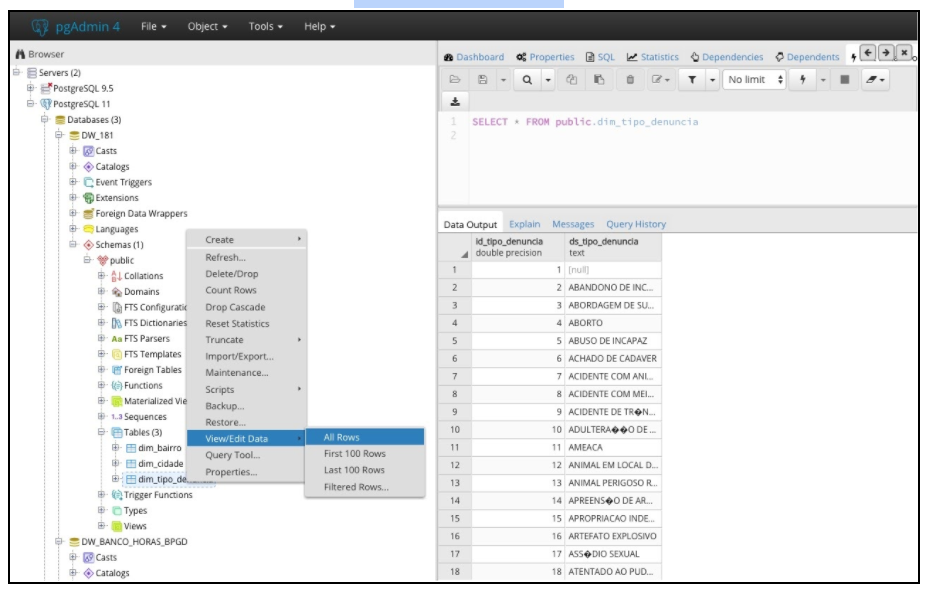
\includegraphics[width=0.6\textwidth]{./04-figuras/figura-res-tipo-denuncia}
    \label{fig:ilustfigrestipodenuncia}
\end{figure}
\vspace*{-0,9cm}
{\raggedright \fonte{Autor desta monografia, 2020.}} \\

% dim_origem
\subsubsection{Criando a transforma\c{c}\~{a}o ``dim\_origem.ktr''}

Os componentes que farão parte da transformação ``dim\_origem.ktr'', serão: \textit{Microsoft Excel Input, Select values, Sort rows, Unique rows, Value Mapper, Add sequence} e finalmente \textit{Table Table output} conforme figura abaixo. 

\begin{figure}[H]
	\vspace*{0,2cm}
    \centering
    \caption{Transformação ``dim\_origem.ktr'' do BI 181}
    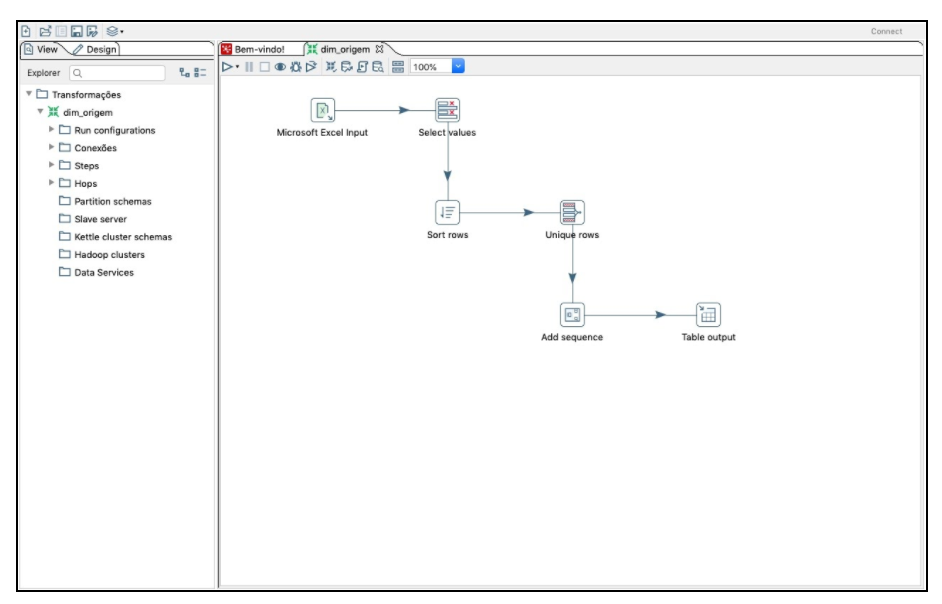
\includegraphics[width=0.6\textwidth]{./04-figuras/figura-dim-origem}
    \label{fig:ilustfigrdimorigem}
\end{figure}
\vspace*{-0,9cm}
{\raggedright \fonte{Autor desta monografia, 2020.}} \\

Primeiramente iremos configurar o \textit{step Select Value} (Selecione o Valor), e na aba \textit{Select & Alter}, na opção \textit{Fields, Rename to}, iremos modificar o nome Bairro para ``ds\_origem'', nesse componente será apenas essa a alteração, conforme figura da tela do \textit{step Select Value}.

Ap/'{o}s componente \textit{Select Value}, iremos configurar o \textit{step Sort rows} (Organizar a linha), na opção \textit{Fields, Ascending} como ``S'', para que os dados fiquem organizado de forma ascendente, figura da tela do \textit{step Sort rows}.

O pr/'{o}ximo componente é \textit{Unique rows} que tem a característica de selecionar apenas os valores únicos das linhas, ou seja, evitar a duplicação, nesse componente há apenas a necessidade de configurar o nome do campo ou \textit{Fieldname}, conforma a figura da tela do \textit{step Unique rows}.

O componente \textit{Value Mapper}, em síntese tem como função trocar os valores vindos da linha da fonte de dados que serão comparados no \textit{Source Value}, e ap/'{o}s encontrar o mesmo ela será trocado pelo informado em \textit{Target value}, conforme a figura da tela do \textit{step Value Mapper}.

Ap/'{o}s transformarmos os dados brutos da linha "origem'' da fonte de dado em \textit{Microsoft Excel}, iremos criar um campo sequencial, para isso usaremos o componente \textit{Add sequence}, a única alteração será no opção Nome do valor, que foi mudado para ``id\_origem'', conforme figura 51 na tela do \textit{Add sequence}.

Finalizando a transformação ``dim\_origem.ktr'', usaremos o componente \textit{Table output} nele iremos alterar as opções \textit{Connection, Target schema, Target table, truncate table}, e na aba \textit{Database fields}, incluiremos os Campos ou colunas da tabela ``dim\_origem'' que será criada ap/'{o}s finalizar essa etapa de configuração dos componentes da transformação, conforme a figura da tela do \textit{step Table output}.

\begin{figure}[H]
	\vspace*{0,2cm}
    \centering
    \caption{Configurando os \textit{steps} da Transformação ``dim\_origem.ktr'' (passo-a-passo)}
    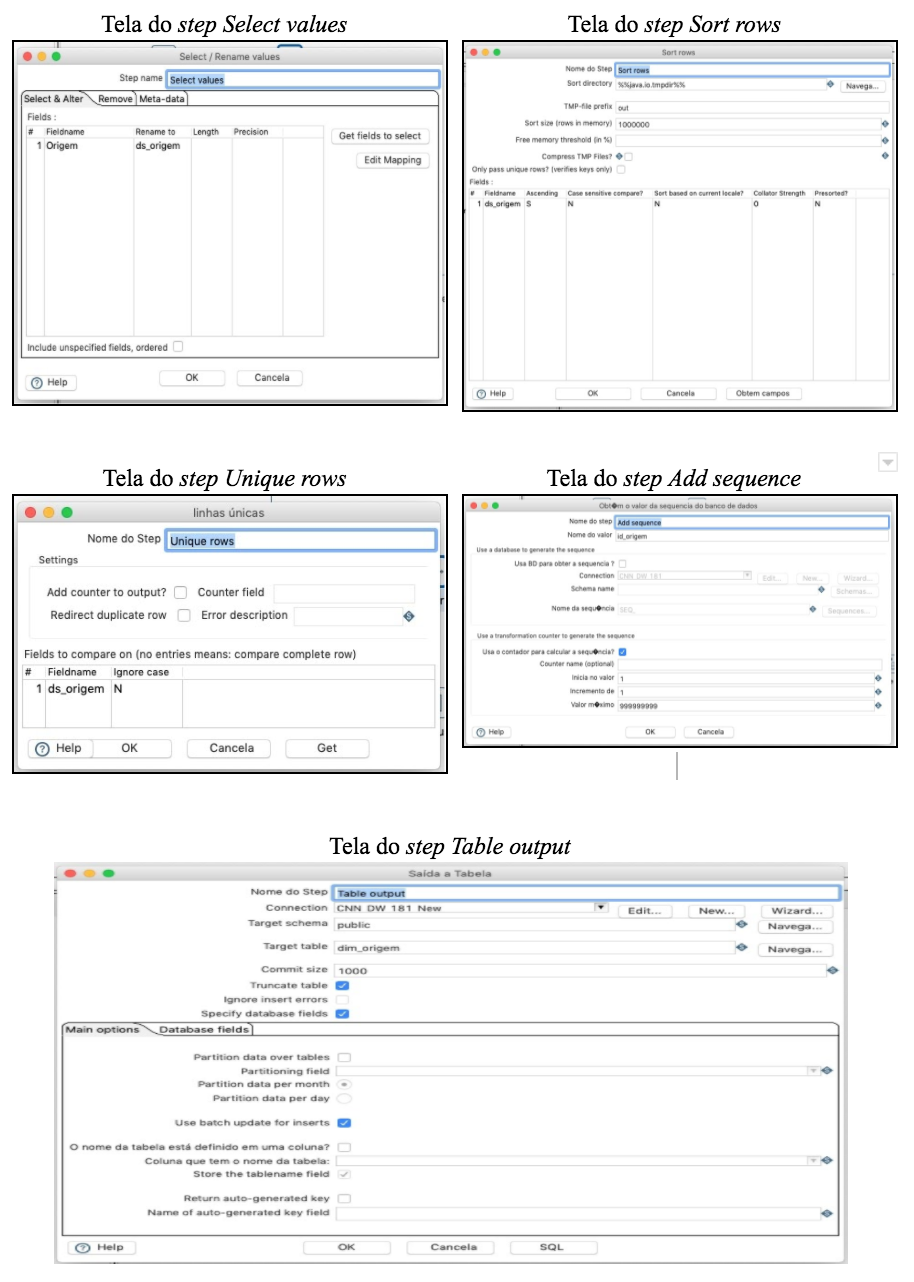
\includegraphics[width=0.6\textwidth]{./04-figuras/figura-dim-origem-passo-a-passo}
    \label{fig:ilustfigdimorigempassoapasso}
\end{figure}
\vspace*{-0,9cm}
{\raggedright \fonte{Autor desta monografia, 2020.}} \\

\begin{figure}[H]
	\vspace*{0,2cm}
    \centering
    \caption{Criando a tabela ``dim\_origem'' no banco de dados usando o \textit{step Table output}}
    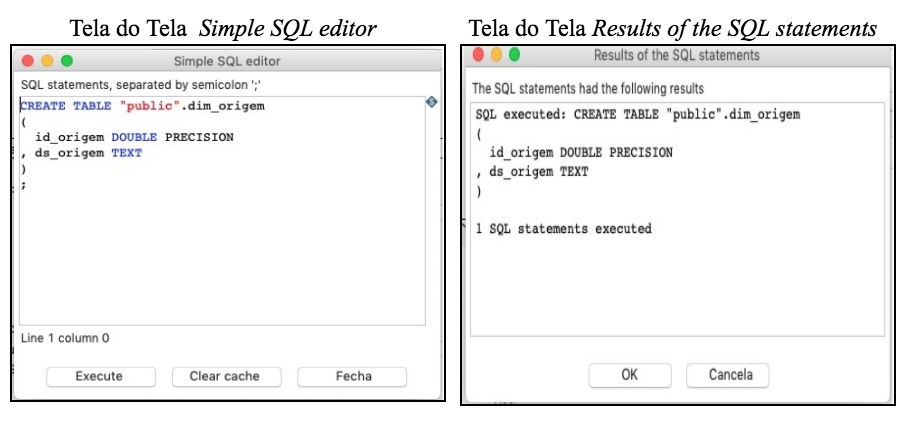
\includegraphics[width=0.6\textwidth]{./04-figuras/figura-tb-dim-origem}
    \label{fig:ilustfigtbdimorigem}
\end{figure}
\vspace*{-0,9cm}
{\raggedright \fonte{Autor desta monografia, 2020.}} \\

Ao final dos processos quando executamos a transformação, conforme figura 53, na parte posterior da tela do PDI, em ``Execution Results''. aparecerá na aba ``Preview data'', os dados padronizados dos campos: ``id\_origem'' e ``ds\_origem''. O pr/'{o}ximo passo será percorrer a grade com os resultado e perceber se o processo de transformação e carga sai conforme planejado. 

\begin{figure}[H]
	\vspace*{0,2cm}
    \centering
    \caption{Executando a transformação ``dim\_origem.ktr''}
    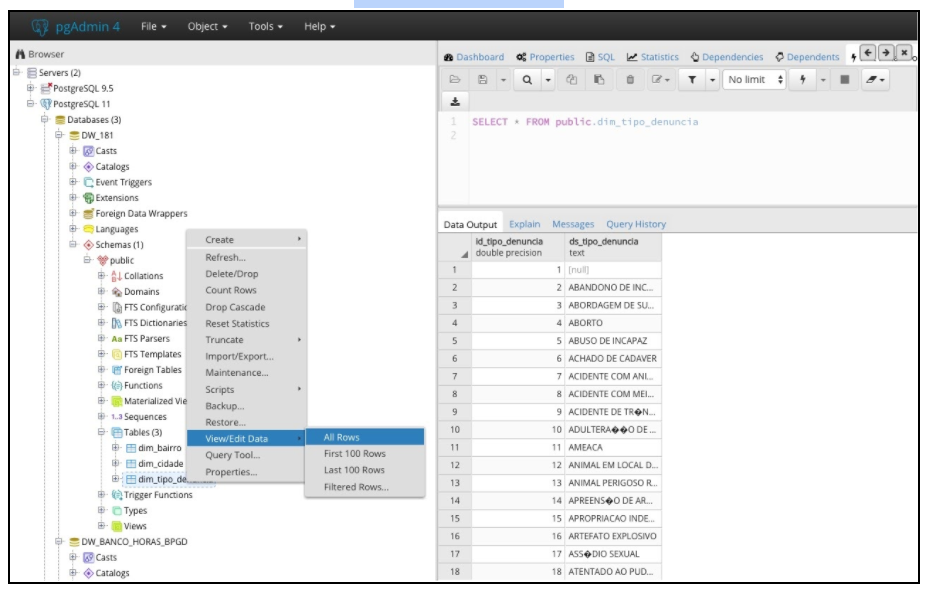
\includegraphics[width=0.6\textwidth]{./04-figuras/figura-res-tipo-denuncia}
    \label{fig:ilustfigrestipodenuncia}
\end{figure}
\vspace*{-0,9cm}
{\raggedright \fonte{Autor desta monografia, 2020.}} \\

Para se ter certeza de que a tabela ``dim\_origem'', obteve a ETL correta, precisamos abrir a tabela ``dim\_origem'' no aplicativo pgAdmin4, que é instalado junto ao PostgreSQL, conforme figura abaixo, nela podemos analisar os dados processados pela transformação criada no PDI: ``dim\_origem.ktr''.

\begin{figure}[H]
	\vspace*{0,2cm}
    \centering
    \caption{Resultado da transformação e carga no Banco de Dados ``DW\_181'' na tabela ``dim\_origem''}
    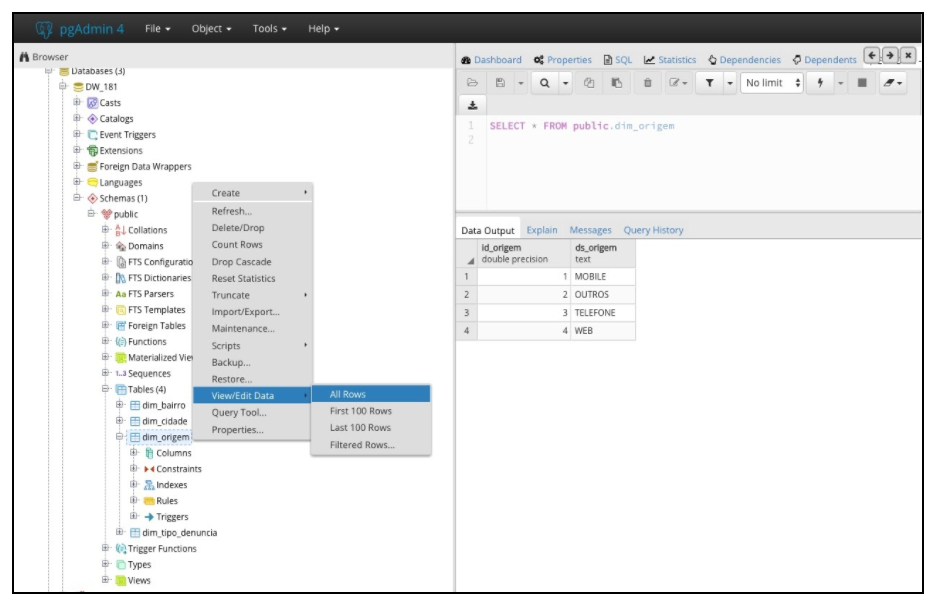
\includegraphics[width=0.6\textwidth]{./04-figuras/figura-res-dim-origem}
    \label{fig:ilustfigresdimorigem}
\end{figure}
\vspace*{-0,9cm}
{\raggedright \fonte{Autor desta monografia, 2020.}} \\

\subsubsection{Criando a transforma\c{c}\~{a}o ``dim\_data.ktr''}

... A FAZER ...

\subsubsection{Criando a transforma\c{c}\~{a}o ``dim\_hora.ktr''}

... A FAZER ...

% FATO
\subsubsection{Criando a transforma\c{c}\~{a}o ``fato\_denuncia.ktr''}

Ap\'os criarmos todas as transforma\c{c}\~{o}es nos t\'opicos anteriores, precisamos criar a transforma\c{c}\~{a}o que criar\'{a} a tabela fato\_denuncia, que ser\'{a} o centro do modelo estrela segundo Machado (2000), conectada com as dimens\~{o}es j\'{a} criadas nas transforma\c{c}\~{o}es dos t\'opicos anteriores.

Na figura abaixo, podemos destacar o uso de um componente novo no contexto desse trabalho, \'{e} o \textit{step Database lookup}, os outros componentes j\'{a} foram usando em t\'opicos anteriores.

\begin{figure}[H]
	\vspace*{0,2cm}
    \centering
    \caption{A transforma\c{c}\~{a}o ``fato\_denuncia.ktr''}
    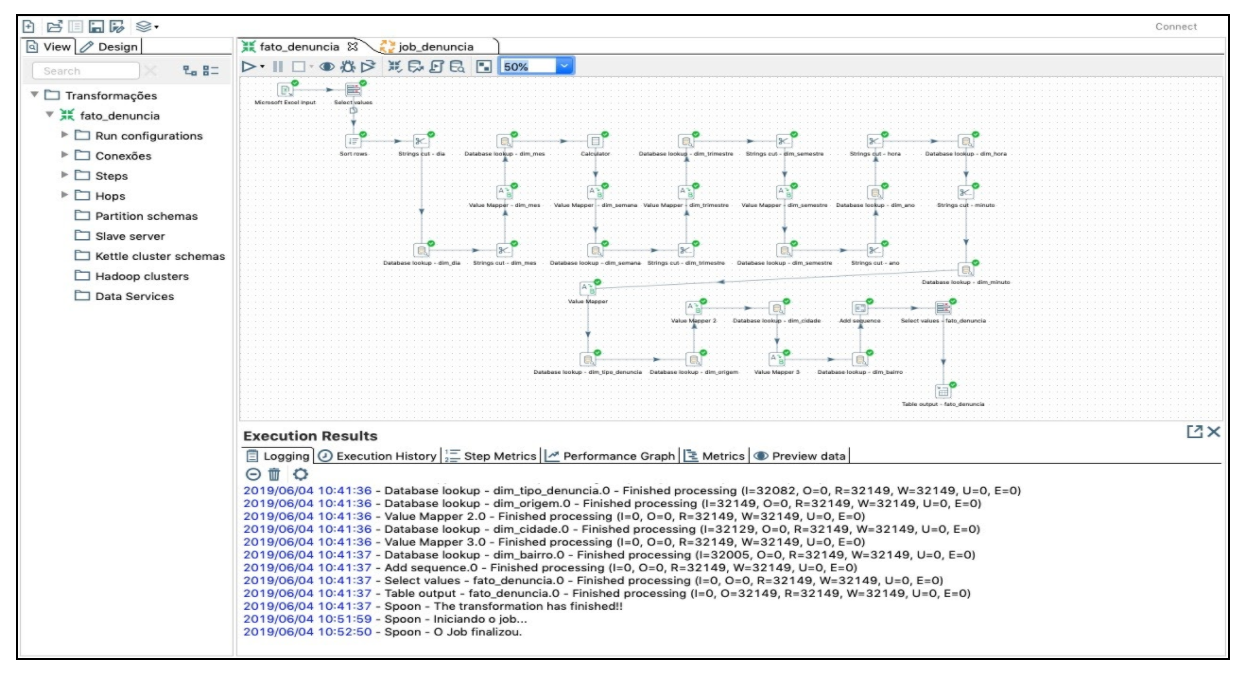
\includegraphics[width=0.6\textwidth]{./04-figuras/figura-fato}
    \label{fig:ilustfigfato}
\end{figure}
\vspace*{-0,9cm}
{\raggedright \fonte{Autor desta monografia, 2020.}} \\

O uso de componente \textit{Database lookup}, \'{e} o detalhe mais importante para que a transforma\c{c}\~{a}o ``fato\_denuncia,ktr'', posso atingir o objetivo principal que \'{e} inserir os dados corretos dentro da tabela ``fato\_denuncia'' dentro do ``DW\_181''. 

O mesmo, precisar ser configurado conforme a abaixo, abaixo, no campo \textit{connection}, deve-se inserir o nome da conex\~{a}o com o SGDB, no campo tabela \testit{Lookup}, devemos determinar a tabela que servir\'{a} de pesquisa no \textit{grid}; a chave(s) para examinar o valor(s): devemos inserir os campos de compara\c{c}\~{a}o na figura abaixo, a compara\c{c}\~{a}o ficou por conta dos campos: ``ds\_dia''  da tabela de pesquisa, na campo do \textit{Grid} ``Campo da tabela'', no campo ``Comparador'', escolhemos a op\c{c}\~{a}o de ``='', e no ``Campo1'', colocamos o campo provindo e configurado no \textit{step Select values}. Quando a compara\c{c}\~{a}o entre os campos \'{e} verificada e encontrada o step retorna o valor configurado no \textit{Grid} Valores a serem retornados da tabela \textit{lookup}, que est\'{a} no campo 
``campo'' do \textit{Grid} acima, conforme figura abaixo.

\begin{figure}[H]
	\vspace*{0,2cm}
    \centering
    \caption{Componente de \textit{Grid step Database Lookup} - ``dim\_dia''}
    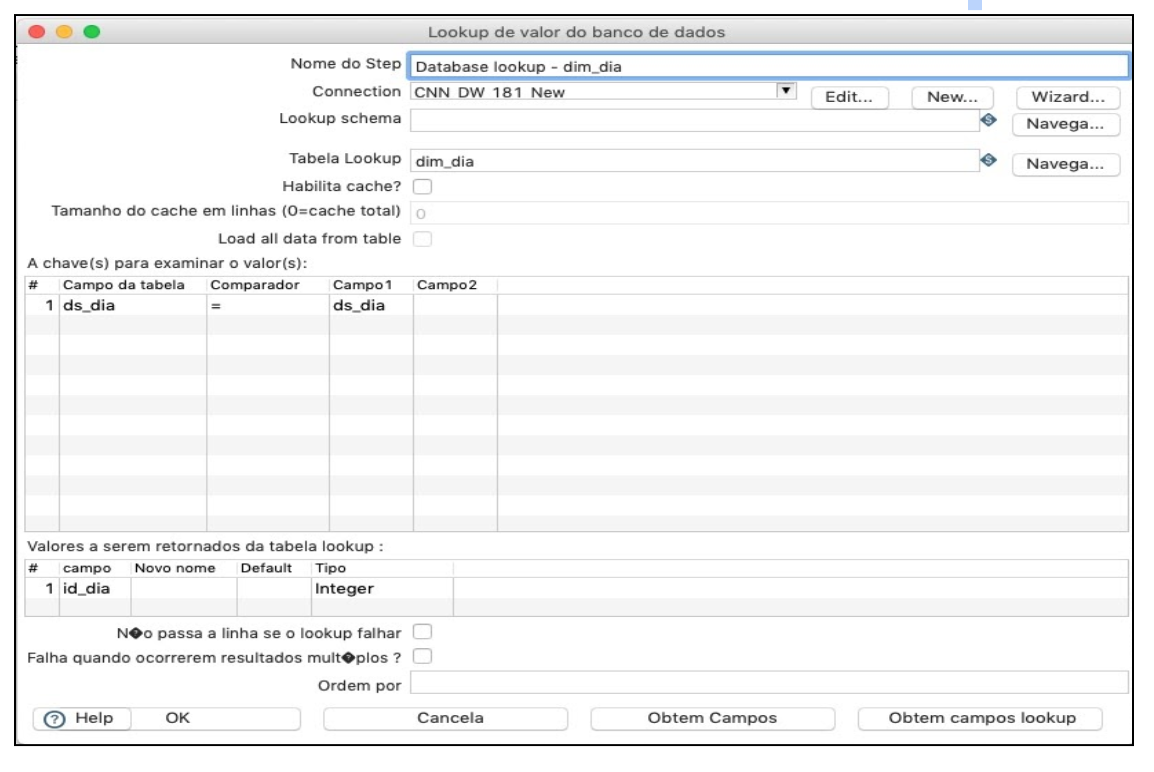
\includegraphics[width=0.6\textwidth]{./04-figuras/figura-dl-dim-dia}
    \label{fig:ilustfigdldimdia}
\end{figure}
\vspace*{-0,9cm}
{\raggedright \fonte{Autor desta monografia, 2020.}} \\

O padr\~{a}o da figura acima ser\'{a} adotada como padr\~{a}o pelos \textit{steps Database lookup} de todas as dimens\~{o}es, sem a necessidade de repetir esses passo aqui nesse t\'opico, assim a tabela de ``fato\_denuncia'' ser\'{a} povoada com os identificadores de cada dimens\~{a}o.

Outra característica da transforma\c{c}\~{a}o ``fato\_denuncia.ktr`` \'{e} o uso do \textit{Step Calculator}, como na figura do t\'opico: "Criando a transforma\c{c}\~{a}o ``dim\_data.ktr'' e  de dois componentes de \textit{step Select values}, o primeiro com os campos do arquivo do ``181.xls'' no formato do textit{Microsoft Excel} e o outro que ap\'os passar por v\'{a}rios \textit{steps} possui os futuros campos da tabela de fato 
``fato\_denuncia'' que ser\'{a} criada e receber\'{a} os dados conforme o processo de ETL configurado nesta transforma\c{c}\~{a}o.

... A FAZER ...

O resultado final da transforma\c{c}\~{a}o ``fato\_denuncia.ktr'', ap\'os ser executada \'{e} apresentada na figura 85, abaixo, \'{e} percebermos os campos da tabela ``fato\_denuncia'', com os c\'odigos de cada tabela de dimens\~{a}o.
Assim, o objetivo desta transforma\c{c}\~{o}es foi alcan\c{c}ado.

\begin{figure}[H]
	\vspace*{0,2cm}
    \centering
    \caption{Resultado da transforma\c{c}\~{a}o e carga no Banco de Dados ``DW\_181'' na tabela fato-denuncia}
    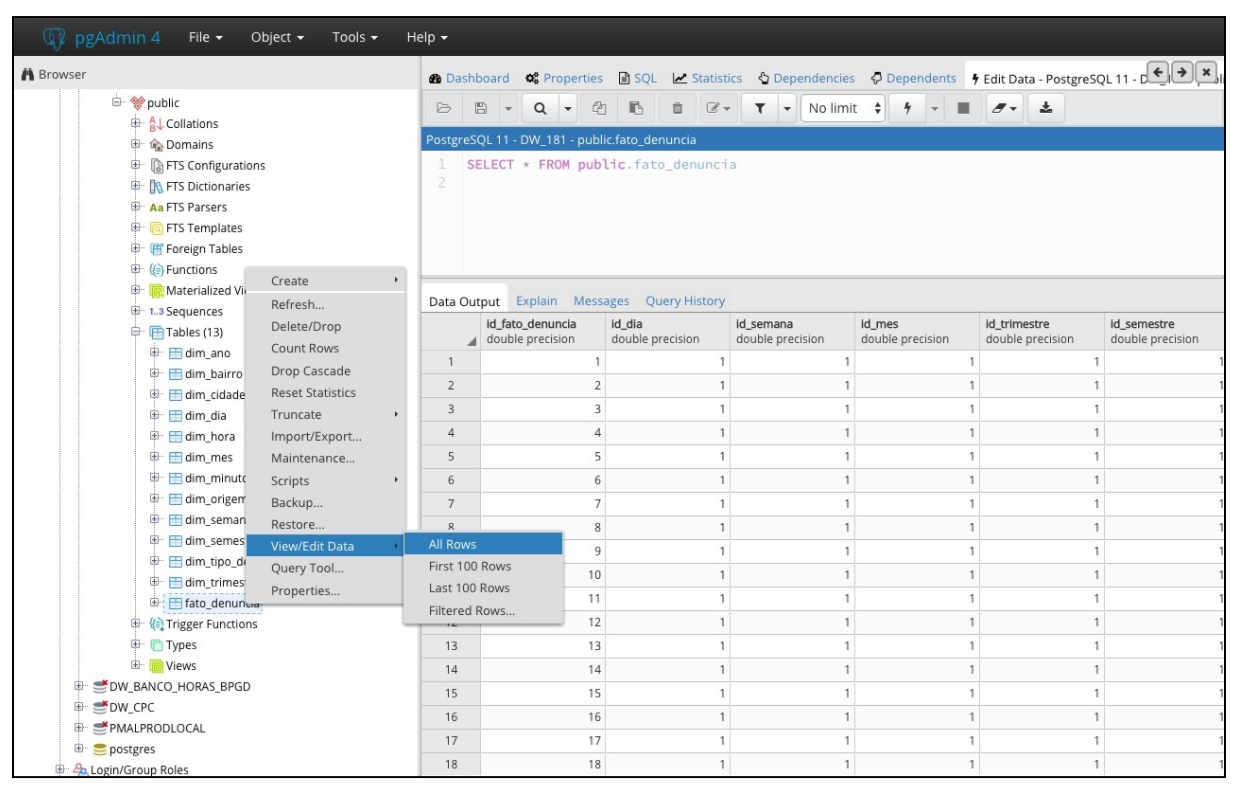
\includegraphics[width=0.6\textwidth]{./04-figuras/figura-resultado-fato-denuncia}
    \label{fig:ilustfigresultadofatodenuncia}
\end{figure}
\vspace*{-0,9cm}
{\raggedright \fonte{Autor desta monografia, 2020.}} \\

% JOBS
\subsubsection{Criando o \testit{JOB} (job\_denuncia)}

Ap\'os termos todas as transforma\c{c}\~{o}es serem criadas e devidamente testadas, faz-se necess\'{a}rio unir todas as transforma\c{c}\~{o}es das dimens\~{o}es e a do fato em processo o "Job" e nomeado como: ``job\_denuncia.kjb''. 

A \textit{priori} inserimos o componente \textit{start} e logo ap\'os cada transforma\c{c}\~{a}o lembrando que o último ser\'{a} o (\textit{Transformation} - fato-denuncia) conforme \`{a} figura abaixo.

\begin{figure}[H]
	\vspace*{0,2cm}
    \centering
    \caption{\textit{Jobs} ou Tarefas ``job\_denuncia.kjb'') do BI 181}
    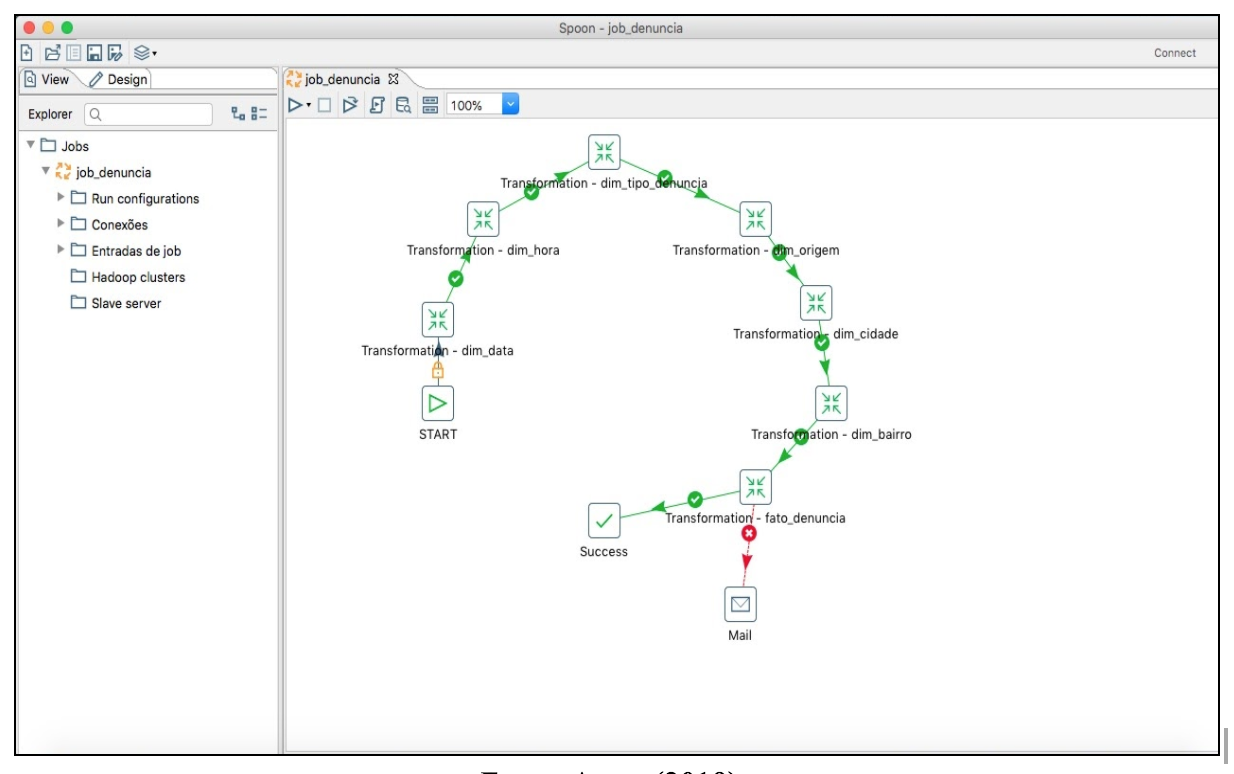
\includegraphics[width=0.6\textwidth]{./04-figuras/figura-job}
    \label{fig:ilustfigjob}
\end{figure}
\vspace*{-0,9cm}
{\raggedright \fonte{Autor desta monografia, 2020.}} \\

Quando executamos o ``job\_denuncia.kjb'', o resultado aparece na tela inferior a \textit{Execution Results} se a execu\c{c}\~{a}o for bem sucedida em cada componente \textit{Transformation} o  componente \textit{Success} aparecer\'{a} conforme a figura abaixo ``Sucesso na execu\c{c}\~{a}o'', abaixo em caso contr\'{a}rio o fluxo ser\'{a} desviado para o componente \textit{Mail} e o componente que obteve o erro ter\'{a} a aparência do figura ``Erro na execu\c{c}\~{a}o de alguma transforma\c{c}\~{a}o''.

% MODELO DIMENSIONAL
\subsubsection{O modelo Dimensional do BI/DW do 181}

Ap\'os a conclus\~{a}o de todas as transforma\c{c}\~{o}es, usando o PDI para desenvolver toda ETL teremos ao final o ``modelo estrela'', conforme figura abaixo, com destaque para o conjunto de dimens\~{o}es que comp\~{o}em o tempo (dim\_ano, dim\_mes, dim\_dia, dim\_semana, dim\_hora, dim\_minuto, dim\_semestre e a dim\_trimestre) que ser\'{a} essencial quando na fase de analíse dos dados usando o \textit{plugin Saiku}. Este modelo \'{e} a base de nosso 
``DW\_181' e atrav\'{e}s dele nosso BI ser\'{a} funcional e poderemos extrair dele as an\'{a}lises que precisaremos para as tomadas de decis\~{o}es.

\begin{figure}[H]
	\vspace*{0,2cm}
    \centering
    \caption{Modelo Dimensional do BI/DW do 181}
    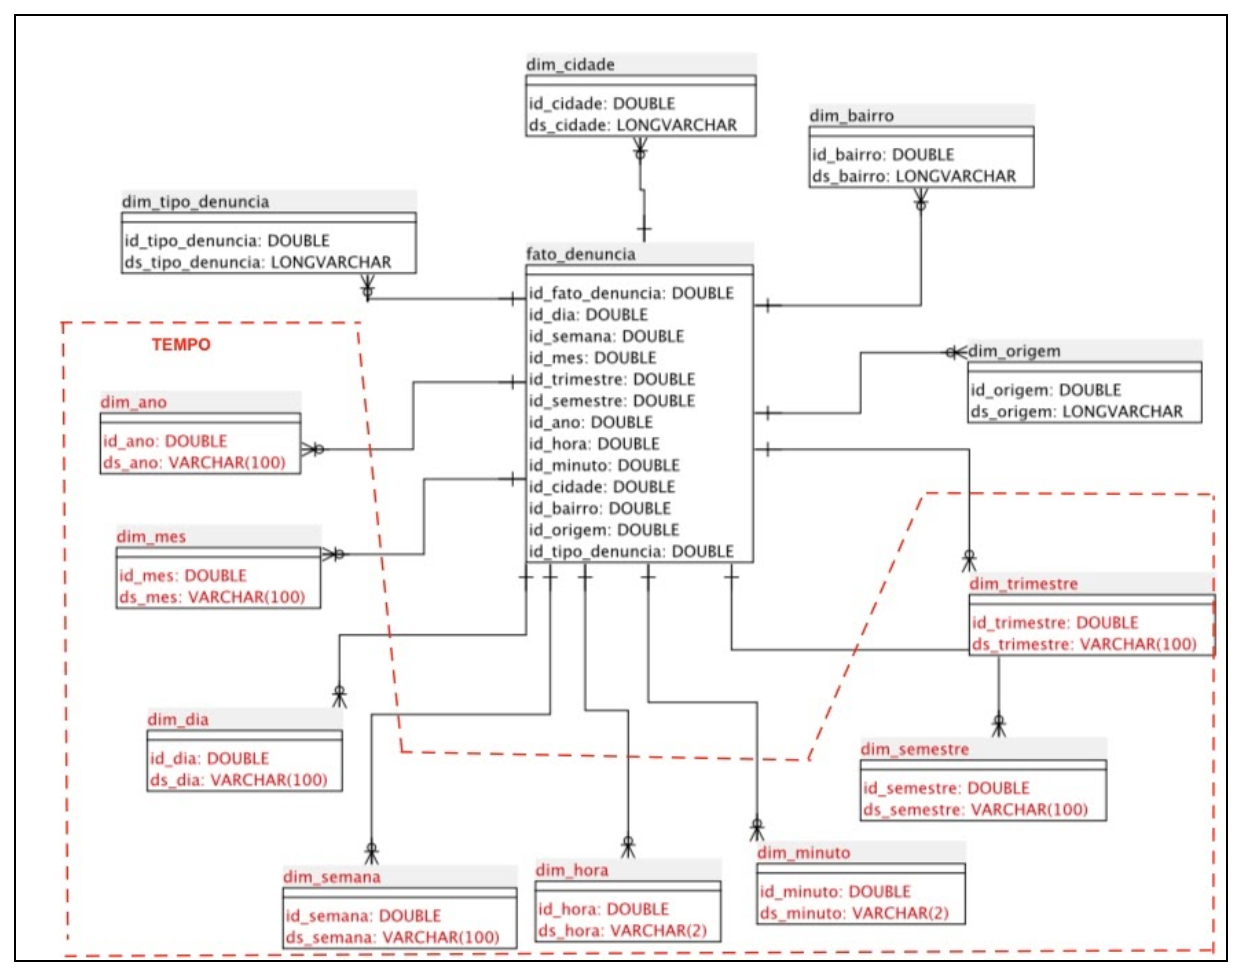
\includegraphics[width=0.6\textwidth]{./04-figuras/figura-moddim}
    \label{fig:ilustfigmoddim}
\end{figure}
\vspace*{-0,9cm}
{\raggedright \fonte{Autor desta monografia, 2020.}} 

% CUBO OLAP
\subsection{Criando o CUBO OLAP}

Em nosso trabalho n\~{a}o iremos nos deter no uso do PSW(\textit{Pentaho Schema Workbench} ou Mondrian), apenas iremos demonstrar como poderemos criar um cubo usando essa ferramenta que faz parte do pacote do Pentaho sem muitos detalhes, pois, podemos criar o cubo dentro do PUC(\textit{Pentaho User Console}), como mostraremos nos pr\'oximos t\'opicos.

\begin{figure}[H]
	\vspace*{0,2cm}
    \centering
    \caption{tela do PSW (\textit{Pentaho Schema Workbench} ou Mondrian)}
    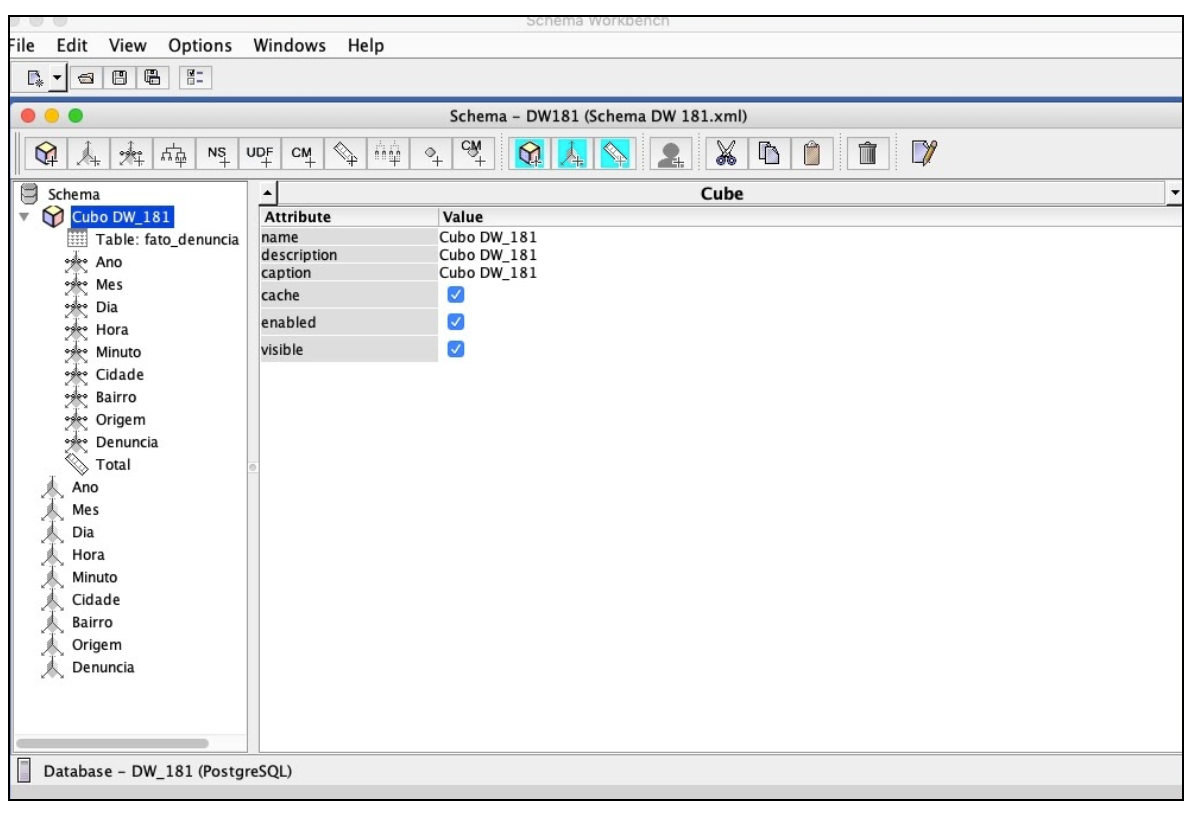
\includegraphics[width=0.6\textwidth]{./04-figuras/figura-pentaho-psw}
    \label{fig:ilustfigpentaho-psw}
\end{figure}
\vspace*{-0,9cm}
{\raggedright \fonte{Autor desta monografia, 2020.}} \\

% PENTAHO
\subsection{Iniciando o Servidor Pentaho}

Ap\'os a fase de ETL utilizando o PDI (Pentaho Data Integration), a mesma sendo testada no SGBD Postgres, e logo ap\'os a cria\c{c}\~{a}o do cubo atrav\'{e}s do PSW (\textit{Pentaho Schema Workbench}) iremos para a fase de implementa\c{c}\~{a}o do BI com objetivo de usarmos o PUC (\textit{Pentaho User Console}).

Inicialmente executaremos o servidor \textit{Tomcat} conforme a figura 90, e para isso devemos usar o terminal em linha de comando do Sistema Operacional MacOSX Catalina, e nos direcionando via comando do console para a pasta:

"Applications/Pentaho/pentaho-server" usando o comando "cd" e se localizar na pasta "pentaho-server", usaremos o comando: "./start-pentaho.sh".

\begin{figure}[H]
	\vspace*{0,2cm}
    \centering
    \caption{Comando no Terminal para iniciar o servidor \textit{Tomcat}.}
    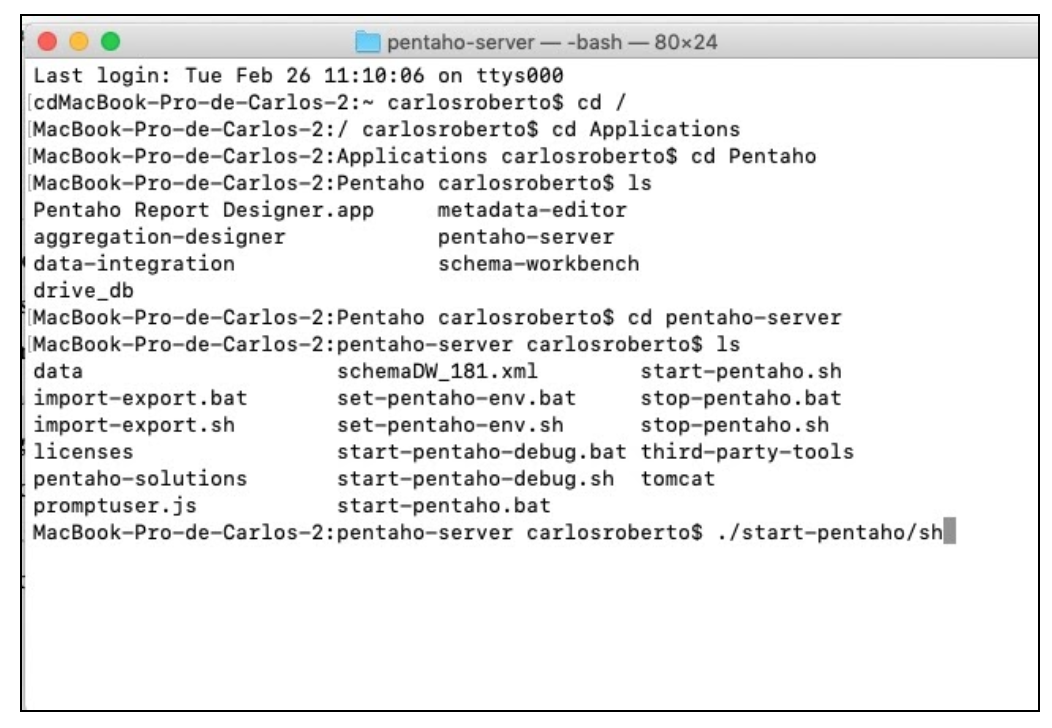
\includegraphics[width=0.6\textwidth]{./04-figuras/figura-pserver}
    \label{fig:ilustfigpserver}
\end{figure}
\vspace*{-0,9cm}
{\raggedright \fonte{Autor desta monografia, 2020.}} \\

Ap\'os executarmos o comando do par\'{a}grafo anterior a aparece na tela do console as informa\c{c}\~{o}es de conex\~{a}o com o servidor \textit{Tomcat}, conforme figura logo abaixo.

\begin{figure}[H]
	\vspace*{0,2cm}
    \centering
    \caption{Comando no Terminal para iniciar o servidor \textit{Tomcat}.}
    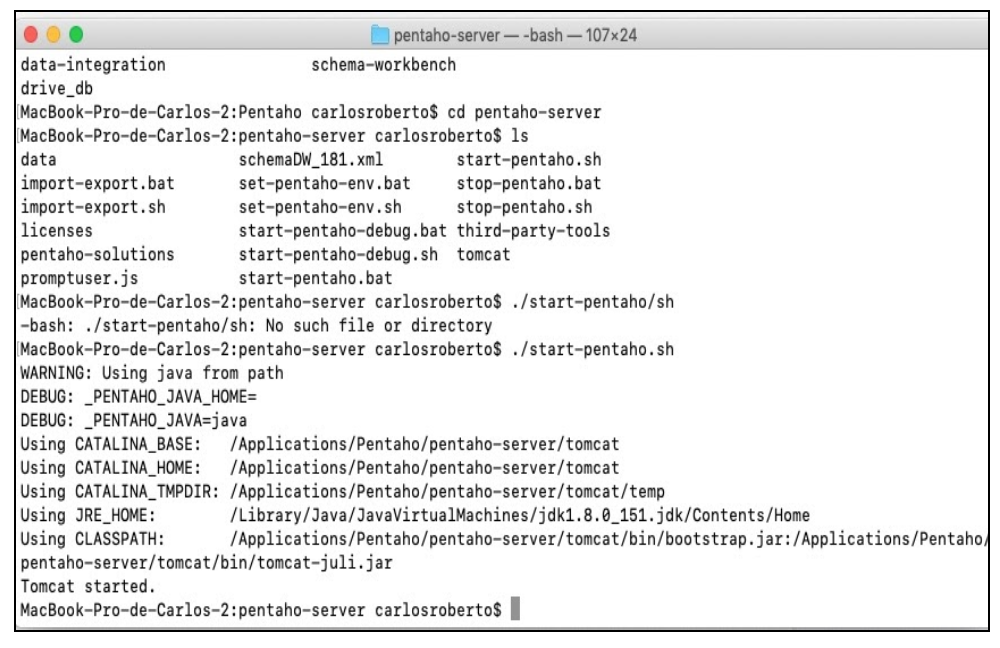
\includegraphics[width=0.6\textwidth]{./04-figuras/figura-pserver-iniciando}
    \label{fig:ilustfigpserveriniciando}
\end{figure}
\vspace*{-0,9cm}
{\raggedright \fonte{Autor desta monografia, 2020.}} \\

Ap\'os os procedimentos e comandos realizados nos par\'{a}grafos acima, devemos acompanhar o pr\'oximo t\'opico destinado ao uso do PUC (\textit{Pentaho User Console}).

% PUC

\subsection{Utilizando o PUC}

O princípio do uso do \textit{Pentaho User Console} tem a similaridade de quando usamos as ferramentas de gerenciamento de arquivos ou qualquer navegador da Web, \'{e} como se estiv\'{e}ssemos usando o PUC. \'{e} essa a analogia em rela\c{c}\~{a}o ao Console de Usu\'{a}rios Pentaho (PUC) que devemos ter em mente para usar esse console. Assim para se familiarizar com as diferentes p\'{a}ginas e controles da PUC, nesse t\'opico iremos detalhar seu uso de uma forma simplificada seguindo o padr\~{a}o do manual do Pentaho (2020).

Primeiramente iniciaremos o navegador que pode ser qualquer um, por\'{e}m, em nosso trabalho iremos usar o navegador web denominado Safari, que \'{e} o padr\~{a}o dos SOs, iOS e macOSX da Apple, e usaremos a URL do servidor Pentaho em nosso trabalho ser\'{a}: "http://localhost:8080".  Ao digitarmos a p\'{a}gina carrega uma tela introdut\'oria com uma se\c{c}\~{a}o de login, como na figura , abaixo.

\begin{figure}[H]
	\vspace*{0,2cm}
    \centering
    \caption{tela do PUC (\textit{Pentaho User Console})}
    \includegraphics[width=0.6\textwidth]{./04-figuras/figura-puc}
    \label{fig:ilustfigpuc}
\end{figure}
\vspace*{-0,9cm}
{\raggedright \fonte{Autor desta monografia, 2020.}} \\

% PENTAHO REPORT DESIGER

\subsection{Utilizando o \textit{Pentaho Report Designer}}

O Report Designer \'{e} uma das v\'{a}rias maneiras de criar relat\'orios com o software Pentaho. Em nosso trabalho, n\~{a}o iremos nos deter nessa ferramenta. Basta apenas saber que, por meio do console do usu\'{a}rio Pentaho baseado na Web do servidor Pentaho, poderemos usar a interface de relat\'orios interativos ou integrar o mecanismo de relat\'orios Pentaho (no qual o \textit{Report Designer} \'{e} construído) ao seu pr\'oprio software.

Para criar um relat\'orio no \textit{Report Designer}, precisamos seguir estes passos:

\begin{itemize}
    \item Conecte-se a uma fonte de dados (geralmente um banco de dados, mas você tamb\'{e}m pode extrair dados de um arquivo simples);
    \item Obtenha seus dados com uma consulta;
    \item Organize os elementos de dados no espa\c{c}o de trabalho do \textit{Report Designer};
    \item Aplique a formata\c{c}\~{a}o aos elementos do relat\'orio;
    \item Adicione elementos do gr\'{a}fico;
    \item Crie f\'ormulas ou campos calculados usando os dados recuperados da sua consulta;e;finalmente;
    \item Publique o relat\'orio no servidor Pentaho ou localmente como um PDF ou outro formato de arquivo suportado. 
\end{itemize}

Assim quando criamos um relat\'orio ele consistir\'{a} principalmente de dados recuperados de uma consulta ao banco de dados que você criar\'{a} atrav\'{e}s do Assistente de Design de Relat\'orios, \textit{SQL Query Designer}, \textit{MQL Query Builder} ou manualmente. 

Depois de ter um conjunto de dados, você pode restringi-lo ainda mais para mostrar detalhes específicos e depois passar para o layout e design do relat\'orio. Na figura abaixo, temos a janela \textit{Welcome} (bem-vindo).

\begin{figure}[H]
	\vspace*{0,2cm}
    \centering
    \caption{tela \textit{Welcome do Pentaho Report Designer}}
    \includegraphics[width=0.6\textwidth]{./04-figuras/figura-welcome-prd}
    \label{fig:ilustfigwelcomeprd}
\end{figure}
\vspace*{-0,9cm}
{\raggedright \fonte{Autor desta monografia, 2020.}} \\
 
Na  pr\'oxima figura, temos a tela do PRD, local onde podemos ajustar nossos relat\'orio de acordo com as nossas
necessidades.

Assim quando criamos um relat\'orio ele consistir\'{a} principalmente de dados recuperados de uma consulta ao banco de dados que você criar\'{a} atrav\'{e}s do Assistente de Design de Relat\'orios, \textit{SQL Query Designer}, \textit{MQL Query Builder} ou manualmente. 

Depois de ter um conjunto de dados, você pode restringi-lo ainda mais para mostrar detalhes específicos e depois passar para o layout e design do relat\'orio. Na pr\'oxima figura , temos a tela do PRD, local onde podemos ajustar nossos relat\'orio de acordo com as nossas necessidades.

\begin{figure}[H]
	\vspace*{0,2cm}
    \centering
    \caption{PRD (\textit{Pentaho Report Designer})}
    \includegraphics[width=0.6\textwidth]{./04-figuras/figura-pentaho-prd}
    \label{fig:ilustfigpentahoprd}
\end{figure}
\vspace*{-0,9cm}
{\raggedright \fonte{Autor desta monografia, 2020.}} \\

% DASHBOARDS

\subsection{Criando \textit{Dashboards}}

Para construirmos nossos \textit{Dashboards} precisaremos utilizar o  Community Dashboard Editor (CDE) e suas tecnologias subjacentes (CDF, CDA e CCC) permitem o r\'{a}pido desenvolvimento e implementa\c{c}\~{a}o dos pain\'{e}is do Pentaho CTools. 

A ferramenta CDE foi criada para simplificar os processos de cria\c{c}\~{a}o, design e renderiza\c{c}\~{a}o dos pain\'{e}is do CTools.

O CDE uma ferramenta poderosa e completa, integrando perfeitamente a interface do usu\'{a}rio com fontes de dados e componentes personalizados.

\subsubsection{Utilizando o \textit{Dashboard Designer} e CTools}

O \textit{Community Dashboard Editor} (CDE) ajuda você a criar e adicionar facilmente pain\'{e}is do CTools. A ferramenta CDE \'{e} um editor de painel gr\'{a}fico que fornece acesso aos componentes do painel no \textit{Community Dashboard Framework} (CDF). Essa ferramenta usa uma grade para o layout que permite criar seus pr\'oprios pain\'{e}is sem precisar de muita experiência em JavaScript ou HTML. Antes de come\c{c}ar, certifique-se de ter ativado o plugin CDE.

\begin{figure}[H]
	\vspace*{0,2cm}
    \centering
    \caption{tela do CDE (\textit{Community Dashboard Editor})}
    \includegraphics[width=0.6\textwidth]{./04-figuras/figura-cde}
    \label{fig:ilustfigcde}
\end{figure}
\vspace*{-0,9cm}
{\raggedright \fonte{Autor desta monografia, 2020.}} \\

Usando nossos dados padronizados providos do ``DW\_181'', criamos nossos \textit{Dashboards} o primeiro deles foi o ``Cidades x Denúncias'', conforme figura abaixo. Nele temos na primeira coluna o cruzamento dos dados das cidades, denúncias em um determinado ano.

\begin{figure}[H]
	\vspace*{0,2cm}
    \centering
    \caption{\textit{Dashboard}: ``Cidades x Denúncias''}
    \includegraphics[width=0.6\textwidth]{./04-figuras/figura-dashboard-cxd}
    \label{fig:ilustfigdcxd}
\end{figure}
\vspace*{-0,9cm}
{\raggedright \fonte{Autor desta monografia, 2020.}} \\

O parâmetro passado \'{e} o campo ano, que est\'{a} no combo box, no lado esquerdo e na parte alta desta coluna. Na segunda coluna h\'{a} o cruzamento dos dados das cidades, denúncias e meses das mesmas, com o parâmetro cidade sendo passado nesta coluna.
    %
% Documento: Analise e Discuss\~{a}o
%

\chapter{ANALISE E DISCUSS\~{a}O}

Os resultados obtidos nos estudos das ferramentas do BI Pentaho, foram demonstrados de forma pr\'{a}tica os conceitos de \textit{Business Intelligence} e de suas etapas estudadas no trabalho provando que as ferramentas seguem o conceito de BI. 

O Pentaho pode ser utilizado gratuitamente e posteriormente adquirir bibliotecas pagas, e ao finalizarmos a implementa\c{c}\~{a}o do BI com os dados provindos de uma planilha no formato do \textit{Microsoft Excel}, usamos na implementa\c{c}\~{a}o os conceitos de Kimball e de outros autores especialistas em BI e aplicando estes conhecimentos, obtivemos como resultados um DW com dados organizados no modelo Estrela, que proporciona a extra\c{c}\~{a}o de informa\c{c}\~{o}es \`{a} nível gerencial, criando uma triagem entre os locais que realmente necessita de um Policiamento Ostensivo e Preventivo mais eficiente, e que pode ser executado pelas for\c{c}as de seguran\c{c}a do Estado.

Este BI desenvolvido em nossa monografia serve como uma ferramenta de TI, para ajudar no planejamento e execu\c{c}\~{a}o de um determinado tipo de policiamento, pois, atuar\'{a} na preven\c{c}\~{a}o e n\~{a}o somente após a ocorrência que gera um determinado tipo penal tenha sido registrada, como \'{e} realizada atualmente. 

Este \'{e} o grande diferencial deste BI, que se utiliza dos dados providos do 181, para gerar informa\c{c}\~{o}es úteis que geram conhecimento para uma tomada de decis\~{a}o mais aprimorada.
O que seguimos neste trabalho foi simplesmente usar os recursos de coleta de dados, transforma\c{c}\~{a}o, carga, criar um local para depositar esses dados tratados e depois trabalhar estes dados de acordo com os princípios da inteligência dos negócios e necessidade do usu\'{a}rio final.

E o resultado final foi um BI com informa\c{c}\~{o}es gerenciais que possibilitam tomadas de decis\~{o}es refinadas e precisas para um melhor ajuste no policiamento em determinada regi\~{a}o, conforme Figura abaixo, abaixo, que foi elaborada com parâmetros da cidade, bairro, tipo da denúncia e os anos.

\begin{figure}[H]
	\vspace*{0,2cm}
    \centering
    \caption{Tela do \textit{Saiku} com o CUBO\_DW\_181 (cidade, bairro, tipo da denúncia e os anos)}
    \includegraphics[width=0.6\textwidth]{./04-figuras/figura-saiku-cbta}
    \label{fig:ilustfigscbta}
\end{figure}
\vspace*{-0,9cm}
{\raggedright \fonte{Autor desta monografia, 2020.}} \\

Na figura acima, podemos ter uma compara\c{c}\~{a}o entre os anos de 2017, 2018, 2019 e 2020, de algumas denúncias em um determinado bairro e cidade, essa informa\c{c}\~{o}es podem propiciar para o gestor na \'{a}rea de seguran\c{c}a uma decis\~{a}o de aumentar ou diminuir o policiamento nestas localidades. Todas estas informa\c{c}\~{o}es usando apenas os recursos do \textit{Plugin Saiku}.

Explorando mais ainda nosso ``CUBO\_DW\_181'', podemos criar consultas com base nos dias da semana e horas, para que um refor\c{c}o na seguran\c{c}a possa se efetivada. A figura 121, demonstrar essas informa\c{c}\~{o}es e a 122, os gr\'{a}ficos de pizza com os dias da semana e os percentuais de denúncia em uma determinada hora.


\begin{figure}[H]
	\vspace*{0,2cm}
    \centering
    \caption{Tela do \textit{Saiku} com o CUBO\_DW\_181 (tipo de denúncia, semana, ano e hora)}
    \includegraphics[width=0.6\textwidth]{./04-figuras/figura-saiku-tipo-semana-ano-hora}
    \label{fig:ilustfigstsah}
\end{figure}
\vspace*{-0,9cm}
{\raggedright \fonte{Autor desta monografia, 2020.}} \\


Com o uso deste BI, teremos muitas possibilidades de cruzamento de dados conforme o surgimentos da necessidades de informa\c{c}\~{o}es, estes últimos gr\'{a}ficos abaixo na Figura, s\~{a}o exemplos desta possibilidades.

\begin{figure}[H]
	\vspace*{0,2cm}
    \centering
    \caption{Tela do \textit{Saiku} - CUBO\_DW\_181}
    \includegraphics[width=0.6\textwidth]{./04-figuras/figura-saiku-pizza}
    \label{fig:ilustfigspizza}
\end{figure}
\vspace*{-0,9cm}
{\raggedright \fonte{Autor desta monografia, 2020.}} \\

Observado estas últimas figura percebemos que temos inúmeras possibilidades usando o ``CUBO\_DW\_181'',  criando assim os cruzamentos dos dados e gerando consultas de acordo com as necessidades de resolu\c{c}\~{a}o de problemas ligados ao excesso de denúncia em em um determinado local e espa\c{c}o de tempo.
      
    %
% Documento: Estrutura
%

\chapter{CONSIDERA\c{c}\~{o}ES FINAIS}

% Sugere-se que este Capítulo 6 seja descrito em dois subtítulos ou se\c{c}\~{o}es: 6.1 - Conclus\~{o}es e  6.2 - Sugest\~{o}es para Trabalhos Futuros, que ser\~{a}o detalhados a seguir.

\section{Conclus\~{o}es}

% Nesta primeira se\c{c}\~{a}o o autor deve sintetizar as principais conclus\~{o}es do trabalho (como um todo e n\~{a}o apenas de sua aplica\c{c}\~{a}o). Deve tamb\'{e}m comentar se os objetivos geral e específicos, descritos no capítulo de introdu\c{c}\~{a}o do trabalho, foram alcan\c{c}ados, total ou parcialmente. 

% Deve comentar, ainda, os seguintes pontos: (i) se a pergunta de pesquisa formulada no Capítulo 1 foi ou n\~{a}o respondida; (ii)  avaliar se os resultados obtidos foram satisfat\'{o}rios; (iii) ressaltar os principais pontos fortes e fracos da solu\c{c}\~{a}o proposta; (iv) descrever os novos conhecimentos que foram adquiridos pela pesquisa, entre outros.

Neste trabalho aplicamos os conhecimentos obtidos com as literatura descritas no t\'{o}pico Fundamenta\c{c}\~{a}o, e focalizamos mais nos conceitos de Kimball (2013), e nos assuntos como: Extra\c{c}\~{a}o Transforma\c{c}\~{a}o e Carga (ETL), granularidade de dados, modelagem multidimensional, \textit{Data Warehouse}, reposit\'{o}rio de dados (\textit{Data Mart} e o CUBO.

Com a base formada nestas teorias, desenvolvemos um BI Básico passo-a-passo, por\'{e}m, bastante funcional aplicando os conceitos de inteligencia de neg\'{o}cio, usando ferramentas modernas de \textit{Business Intelligence}, com destaque para a Plataforma de Integra\c{c}\~{a}o de Dados e Análise Pentaho da Empresa Hitachi.

A solu\c{c}\~{a}o final pode ser usada para ajudar gestores da área de seguran\c{c}a pública, pois, trata os dados diversos advindos de um Sistema Operacional que recebe informa\c{c}\~{o}es do servi\c{c}o 181 do Estado de Alagoas. 

O BI deste trabalho processa esses dados e transforma em gráficos e pain\'{e}is funcionais, que podem ser usados para a m\'{e}trica de eventos relacionados ao uso aprimorado dos servi\c{c}o de policiamento ostensivo no âmbito da seguran\c{c}a publica estadual e municipal.

\section{Sugest\~{o}es para Trabalhos Futuros}
% Um estudo de técnicas de treinamento será interessante a trabalhos futuros.
% Outro ponto de aplicação de BI que pode ser explorado que se torna muito interessante é a área de BSC, envolvida não somente a indicadores, mas com plano de ação de acordo com a realização das metas destes indicadores.

Com este trabalho, estamos iniciando uma jornada para uma sistematiza\c{c}\~{a}o com base na inteligencia de neg\'{o}cio e que ela possa ajudar vários setores da nossa sociedade.

Nossa sugest\~{a}o para trabalhos futuros \'{e} maie técnicas de BI sejam aprimoradas e que elas inovem mais rapidamente com produto de gerenciamento de dados para análises, IA e integra\c{c}\~{a}o de dados e desenvolva sua prática de DataOps \index{DataOps}\footnote{DataOps: \'{e} uma metodologia automatizada, orientada a processos, usada por equipes analíticas e de dados, para melhorar a qualidade e reduzir o tempo de ciclo da análise de dados}. 

Com essa inova\c{c}\~{a}o sugerida esperamos que haja melhorias nas opera\c{c}\~{o}es de dados em todos os lugares Simplificando suas opera\c{c}\~{o}es de dados e forne\c{c}a acesso a informa\c{c}\~{o}es para todas as partes interessadas de uma organiza\c{c}\~{a}o com automa\c{c}\~{a}o baseada em políticas e gerenciamento de dados orientado por metadados.

    
    % Elementos pós textuais
    \postextual
    %
% Documento: Referências Bibliográficas
%

\bibliography{refbase}    % Geração automática das referências por meio do arquivo 'refbase.bib'
       % Referências
    %%
% Documento: Apêndices
%

\begin{apendicesenv}

\chapter{Como elaborar}

Apêndice é texto ou documento elaborado pelo autor, a fim de
complementar sua argu-mentação, sem prejuízo da unidade nuclear do trabalho. Documentos elaborados por vários au-tores, com um responsável intelectual destacado (organizador, coordenador Elemento opcional.  Deve ser precedido da palavra APÊNDICE, identificado por letras maiúsculas consecutivas, travessão e pelo respectivo título. Utilizam-se letras maiúsculas dobradas, na identificação dos apêndices, quando esgotadas as letras do alfabeto.

\end{apendicesenv}
         % Apêndices
    %%
% Documento: Anexos
%

\begin{anexosenv}

\chapter{Como elaborar}

Anexo é texto ou documento não elaborado pelo autor, que serve de fundamentação, comprovação e ilustração. Elemento opcional. Deve ser precedido da palavra ANEXO, identifi-cado por letras maiúsculas consecutivas, travessão e pelo respectivo título. Utilizam-se letras maiúsculas dobradas, na identificação dos anexos, quando esgotadas as letras do alfabeto.


\end{anexosenv}            % Anexos
    %\printindex                                             % Índice remissivo

\end{document}
